% This is the Reed College LaTeX thesis template. Most of the work
% for the document class was done by Sam Noble (SN), as well as this
% template. Later comments etc. by Ben Salzberg (BTS). Additional
% restructuring and APA support by Jess Youngberg (JY).
% Your comments and suggestions are more than welcome; please email
% them to cus@reed.edu
%
% See http://web.reed.edu/cis/help/latex.html for help. There are a
% great bunch of help pages there, with notes on
% getting started, bibtex, etc. Go there and read it if you're not
% already familiar with LaTeX.
%
% Any line that starts with a percent symbol is a comment.
% They won't show up in the document, and are useful for notes
% to yourself and explaining commands.
% Commenting also removes a line from the document;
% very handy for troubleshooting problems. -BTS

% As far as I know, this follows the requirements laid out in
% the 2002-2003 Senior Handbook. Ask a librarian to check the
% document before binding. -SN

%%
%% Preamble
%%
% \documentclass{<something>} must begin each LaTeX document
\documentclass[12pt,twoside]{reedthesis}
% Packages are extensions to the basic LaTeX functions. Whatever you
% want to typeset, there is probably a package out there for it.
% Chemistry (chemtex), screenplays, you name it.
% Check out CTAN to see: http://www.ctan.org/
%%
\usepackage{graphicx,latexsym}
\usepackage{amsmath}
\usepackage{amssymb,amsthm}
\usepackage{longtable,booktabs,setspace}
\usepackage{chemarr} %% Useful for one reaction arrow, useless if you're not a chem major
\usepackage[hyphens]{url}
% Added by CII
\usepackage{hyperref}
\usepackage{lmodern}
\usepackage{float}
\floatplacement{figure}{H}
% End of CII addition
\usepackage{rotating}

% Next line commented out by CII
%%% \usepackage{natbib}
% Comment out the natbib line above and uncomment the following two lines to use the new
% biblatex-chicago style, for Chicago A. Also make some changes at the end where the
% bibliography is included.
%\usepackage{biblatex-chicago}
%\bibliography{thesis}


% Added by CII (Thanks, Hadley!)
% Use ref for internal links
\renewcommand{\hyperref}[2][???]{\autoref{#1}}
\def\chapterautorefname{Chapter}
\def\sectionautorefname{Section}
\def\subsectionautorefname{Subsection}
% End of CII addition

% Added by CII
\usepackage{caption}
\captionsetup{width=5in}
% End of CII addition

% \usepackage{times} % other fonts are available like times, bookman, charter, palatino


% To pass between YAML and LaTeX the dollar signs are added by CII
\title{Thesis}
\author{Emily Palmer}
% The month and year that you submit your FINAL draft TO THE LIBRARY (May or December)
\date{May 2018}
\division{Mathematics and Natural Sciences}
\advisor{Andrew Bray}
\institution{Reed College}
\degree{Bachelor of Arts}
%If you have two advisors for some reason, you can use the following
% Uncommented out by CII
% End of CII addition

%%% Remember to use the correct department!
\department{Mathematics}
% if you're writing a thesis in an interdisciplinary major,
% uncomment the line below and change the text as appropriate.
% check the Senior Handbook if unsure.
%\thedivisionof{The Established Interdisciplinary Committee for}
% if you want the approval page to say "Approved for the Committee",
% uncomment the next line
%\approvedforthe{Committee}

% Added by CII
%%% Copied from knitr
%% maxwidth is the original width if it's less than linewidth
%% otherwise use linewidth (to make sure the graphics do not exceed the margin)
\makeatletter
\def\maxwidth{ %
  \ifdim\Gin@nat@width>\linewidth
    \linewidth
  \else
    \Gin@nat@width
  \fi
}
\makeatother

\renewcommand{\contentsname}{Table of Contents}
% End of CII addition

\setlength{\parskip}{0pt}

% Added by CII

\providecommand{\tightlist}{%
  \setlength{\itemsep}{0pt}\setlength{\parskip}{0pt}}

\Acknowledgements{
I want to thank a few people.
}

\Dedication{

}

\Preface{

}

\Abstract{
Classification for authorship of written classical music is a relatively
infrequently explored field. In theory composers leave behind unconsious
(or perhaps consious) signals that indicate a piece of music as thier
own. Ideally these signals, or features can be extracted and used to
build a model to predict the composer of a piece of music. For instance
the siblings Fanny Hensel and Felix Mendelssohn, although very similar
in compositional style, likely have featuresthat distingush their music.
It is speculated that there are at least \ldots{} pieces that Fanny
wrote that were published by Felix. Low level features, including
frequencies of chords and scale degree usage were extracted from
\ldots{} pieces known to be written by Felix and \ldots{} pieces known
to be written by Fanny. These features were extracted using museR, an R
package written by me*. Additionally, to check the validity of the
model, pieces from J.S. Bach's Well Tempered Clavier were used to
compare against Felix and Fanny. A lasso logistic model was then trained
on Bach and Mendelsssohn data using 5-fold cross validation with a
missclassification rate of \ldots{} . A lasso logistic model was then
trained in the same way on Felix and Fanny data with a
missclassification rate of \ldots{} Finally the 12 disputed pieces were
checked and \ldots{}
}

	\usepackage{tikz,amsmath,graphicx,}
	\usetikzlibrary{shapes,arrows}
	\newcommand*{\h}{\hspace{5pt}}% for indentation
	\newcommand*{\hh}{\h\h}% double indentation
% End of CII addition
%%
%% End Preamble
%%
%

\usepackage{amsthm}
\newtheorem{theorem}{Theorem}[chapter]
\newtheorem{lemma}{Lemma}[chapter]
\theoremstyle{definition}
\newtheorem{definition}{Definition}[chapter]
\newtheorem{corollary}{Corollary}[chapter]
\newtheorem{proposition}{Proposition}[chapter]
\theoremstyle{definition}
\newtheorem{example}{Example}[chapter]
\theoremstyle{definition}
\newtheorem{exercise}{Exercise}[chapter]
\theoremstyle{remark}
\newtheorem*{remark}{Remark}
\newtheorem*{solution}{Solution}
\begin{document}

% Everything below added by CII
  \maketitle

\frontmatter % this stuff will be roman-numbered
\pagestyle{empty} % this removes page numbers from the frontmatter
  \begin{acknowledgements}
    I want to thank a few people.
  \end{acknowledgements}

  \hypersetup{linkcolor=black}
  \setcounter{tocdepth}{2}
  \tableofcontents

  \listoftables

  \listoffigures
  \begin{abstract}
    Classification for authorship of written classical music is a relatively
    infrequently explored field. In theory composers leave behind unconsious
    (or perhaps consious) signals that indicate a piece of music as thier
    own. Ideally these signals, or features can be extracted and used to
    build a model to predict the composer of a piece of music. For instance
    the siblings Fanny Hensel and Felix Mendelssohn, although very similar
    in compositional style, likely have featuresthat distingush their music.
    It is speculated that there are at least \ldots{} pieces that Fanny
    wrote that were published by Felix. Low level features, including
    frequencies of chords and scale degree usage were extracted from
    \ldots{} pieces known to be written by Felix and \ldots{} pieces known
    to be written by Fanny. These features were extracted using museR, an R
    package written by me*. Additionally, to check the validity of the
    model, pieces from J.S. Bach's Well Tempered Clavier were used to
    compare against Felix and Fanny. A lasso logistic model was then trained
    on Bach and Mendelsssohn data using 5-fold cross validation with a
    missclassification rate of \ldots{} . A lasso logistic model was then
    trained in the same way on Felix and Fanny data with a
    missclassification rate of \ldots{} Finally the 12 disputed pieces were
    checked and \ldots{}
  \end{abstract}

\mainmatter % here the regular arabic numbering starts
\pagestyle{fancyplain} % turns page numbering back on

\chapter{}\label{section}

\section{Introduction:}\label{introduction}

The purpose of this thesis is to use musical stylometry to quantify the
difference between the compositions of the siblings Felix and Fanny
Mendelssohn. (I hate starting things help\ldots{})

Treating text or music as data has challenges. Neither contains anything
immediately analyzable. With the increasing availability of the internet
and social media data, text classification has become an promising form
of data analysis. While text classification problems are very frequent,
similar methods that classify music have not been as commonly explored.
To exploret these problems, first analyzable features must identified
that can be extracted for every text. These features can include word
frequencies, length etc. Analysis of text using machine learning can
find patterns, authors, or categories of text. Similar methods can also
be used to classify music.

Feature extraction is an essential part in text or music classification.
Unlike in a data set of numerical or categorical values, text and music
must first go through a processing stage where features of interest can
be extracted before any models can be fit.

For music, the extracted features are used to build a model that can
correctly classify a likely composer for that piece of music. Studies
that examine the style of a type of music or composer are known as
musical stylometry studies. For musically trained humans, this might be
an easy task. Some are able to automatically distinguish a piece
composed by Bach or Mozart either by listening to a recording, or
looking at sheet music. This becomes more difficult when composers are
contemporaries. Mozart and Salieri might be distinguishable to a more
discerning listener or scholar, but it might be harder. Harder still is
when the identity of the composer piece of music is disputed. Examples
of such disputed authorship exist throughout music history, most notably
in the Renaissance.

In both text and music classification, we must create features that can
be calculated that would give a signal to indicate some conscious or
unconscious tendency of the composer that would make them
distinguishable.

\section{Brief history of text
classification}\label{brief-history-of-text-classification}

The Federalist Papers were one of the earliest instances of text
classification for determining authorship.(Mosteller \& Wallace, 1964).
The famous Federalist Papers were written under the pen name `Publius'.
There are several of these disputed papers attributed to James Madison
or Alexander Hamilton. The authors never admitted authorship, as some of
the writings were contradictory to their later political positions
(Adair, 1944). Prior to quantitative analysis, historians had often
examined the papers using styles of previously known writings of Madison
and Hamilton. Their analysis was often partially based on the content of
the letters, for example the existence of citing English history is a
trait more common to Hamilton. (Ford \& Bourne, 1897)

In contrast, Mosteller and Wallace (1964) used the frequency of words
such as `and', `by', `from', and `upon', to train the writings on a set
of known writings by each author. These unconscious indicators were able
to differentiate between the two writers, and the model was able to
identify the likely author of the disputed paper.

\section{Feature selection}\label{feature-selection}

Text analysis, such as in the Federalist Papers, is accomplished by
reading one word after another. Information in a piece of music,
however, is read in a variety of ways. It can be read left to right note
by note, but it can also be read vertically as the harmony, or the notes
played together. Also in a piece with several instruments, the above
happens at the same time for each instrument. There are also aspects
that take place over large sections, such as phrasing, or cadential
patterns. There are rules of counterpoint that are followed throughout
the entire piece. Thus we need to find features that can be measured for
each piece, or perhaps each measure or instrument, that can describe a
certain piece of music. Then we must decide which features are those of
rules and practices of classical music, and where the creativeness and
individuality of a composer happens. As there are many different aspects
of a piece, melodic changes, harmonies, etc, one can end up with many
features to describe one piece. It is possible that the number of
predictors \((p)\) can be greater than the sample size \((n)\), or that
many features encode essentially the same thing. We thus need to figure
a clever way to decrease our predictor space. This can happen in
choosing what features we want to use to model, or using a dimension
reduction technique such as PCA.

Most of the classical musical stylometry papers have focused on
composers in the Renaissance(1400-1600), Baroque(1600-1750), and
Classical(1730-1820) eras. The Mendelssohns were composing in the
Romantic era(1780-1910). The focus of earlier papers may have been
because composers in earlier eras followed rules of counterpoint more
exactly, or perhaps had less ``expressive'' allowances for their
composing, thus making features easier. There are also more pieces with
doubtful authorship in those eras. In addition Computer Assisted
Research in the Humanities (CCARH) has a large corpus of encoded music
from these times. As will be described later, the initial step of coding
the music is the most time consuming, having music in a format
immediately conducive to analysis is very helpful.

\section{A Very Short Introduction to Music
Theory}\label{a-very-short-introduction-to-music-theory}

Western sheet music is presented on a five line staff. The vertical
distance between notes (also known as an interval) depends on how many
half steps occur between two notes. There are 12 half steps in the
western scale. Melodic intervals are defined as the number of half steps
between two adjacent notes. Harmonic intervals are defined as the number
of half steps between notes played at the same time. Chords occur when
there are more than two notes being played simultaneously. The type of
chord is also determined by the harmonic intervals it contains. Cadences
are a type of chord progression, usually occurring at the end of a
phrase and especially at the end of a piece. Musical notes are in the
set \(\text{note} \in \{A,B,C,D,E,F,G\}\). The value of a note can be
changed up or down a half step, by adding a sharp or flat. The key
signature of the piece indicates how many sharps or flats are normal for
the piece. A piece's key can be major or minor, although the piece can
internally modulate between the two. The scale degree of a note depends
on its position of the key that it is in. The time signature of a piece
determines the number of beats that are in each measure. Intervals and
chords can be either dissonant or consonant. Consonant intervals sound
nice to our ears, whereas dissonant intervals add a sense of tension or
unease, which is used to shape the feel of the music. In addition chords
and intervals can be minor or major. Minor intervals feel ``sad'',
whereas major intervals feel ``happy''. These are also known as
sonorities, and divided into three types. Imperfect sonorities
are\ldots{} perfect sonorities are \ldots{} and and dissonant sonorities
are..

For classical music there are some ``rules'' that most composers follow
to some extent. These were followed more strictly in the Baroque era
than the Romantic era. These rules are known as counterpoint. First
species counterpoint is a type of counterpoint. One rule is that there
are no parallel perfect consonances. Perfect consonances are octaves,
fourths and fifths. Parallel indicates that they occur one after
another. Another rule is that from one perfect consonance to another,
the notes must proceed in contrary or oblique motion.

\section{Musical features}\label{musical-features}

Features calculated from music often closely follow music theory. In
music, in addition to deciding the features, there is also the decision
of the scope at where those features take place. They can be features
for a given instrument, the entire piece, or each measure. Also
windowing techniques can be used where a ``window'' is created over a
given number of bars or notes, and shifts across the whole piece For
each window, a feature is recorded. These can be overlapping windows by
creating an ``offset'' of a number of beats or notes. Windowing produces
more data, as instead of one feature for each piece, there is a feature
for each window.

Musical features are often thought about as either high level, or low
level. While the exact definition of each often varies, low level is
often understood to be features such as note frequency, etc. High level
features are more about a broader sense of the piece, including chord
progressions, etc. High level features are often what music experts use
in their analysis, whereas low-level features are more easily done with
computer analysis. High level features often depend on the context of
where the features was extracted from. For example, cadences and
modulations (brief changes in key) throughout the piece are easily found
when a human analyzes a piece of music, but are very hard to generalize
as a feature. If one wants to use high-level features, they would first
have to train the feature to see if it was performing accurately. For
this reason, this paper focuses only on low level pieces, or pieces that
are context independent.

Especially in research regarding text categorization, data sets have
enormous numbers of variables. We use ``feature'' and ``variable''
interchangeably, with the exception when features are created from
variables, and the distinction will be made in that case (Guyon \&
Elisseeff, 2003). There are several variable selection algorithms that
select the ``important'' variables. If one included every variable that
was extracted from a piece, the model would very likely be overfit. Thus
some feature selection is important before fitting a model.

\section{Background on Variable and Feature
Selection}\label{background-on-variable-and-feature-selection}

Before analysis is done, numerous features are often extracted from the
music without knowing a priori which ones will be helpful in identifying
a composers' style. Thus we have to choose which features we want to use
in our model. There are many ways to do this and existing variable
selection algorithms can help with this process.

Variable ranking uses a score function to assign a score to each
possible variable. It is a computationally efficient method and is
robust against overfitting as it introduces bias but may result in less
variance. It is tempting to only include variables that have a high
score. However, this possibly leads to redundancy. In addition,
variables that are not important by themselves can have a significant
performance improvement when considered with other variables.

Single variable classifiers rank the variable according to its
individual predictive power. The predictive power can be measured in
terms of error rate, or using the false positive or false negative rate.
This classifier cannot distinguish variables that perfectly separate the
data.

After knowing the ranking of a variable, we then select which variables
will be useful for our model. This is known as variable subset
selection. The three most common types of variable subset selection are
filters, wrappers, and embedded methods. Filters do not involve any
machine learning to create the criteria for variable subset selection.
Wrappers on the other hand use the resulting performance from training a
given features subset. Embedded methods perform variable selection in
the process of training a model and are usually specific to given
learning machines. **

All possible subsets of variables is \(2^p-1\), which for large \(p\) is
often computationally impossible. Strategies like best-first, branch and
bound, simulated annealing, and genetic algorithms can help with the
computational difficulties.

Dimensional reduction is also commonly used to combine enough of the
information given in the features in a smaller dimensional space. This
results in feature creation; using the recorded variables to create new
features to fit the model on. Dimensional reduction techniques include
include clustering and PCA/SVD. The two goals of these feature creations
are that we can achieve a good reconstruction of the data. The second is
that we can be successful in making our predictors. The first is an
unsupervised problem. The second is supervised.

\section{Previous research.}\label{previous-research.}

There have been numerous other applications of machine learning to
music. For example, a previous study used machine learning trained on a
composer's music to have the computer learn the style and and compose a
piece in a similar style. (Papadopoulos \& Wiggins, n.d.)

Research on musical stylometry has focused on two types of data: audio
and sheet music. This analysis uses data in the form of sheet music. To
predict a composer, a training data set of pieces of known composer is
needed. Then a model can be fit to a testing data set to predict
composer. If the fitted model shows good predictions, that model can be
used on the pieces of unknown authorship. Musical stylometry can be used
to resolve disputed authorship, but also to detect distinguishing
musical styles of composer, even if there are no disputed pieces. This
same process can also be used to look at the development of a composers
musical style over time.

To my knowledge there are currently four studies that have looked at the
question of classifying composers by extracting features from sheet
music. Several previous papers have focused on Josquin des Prez. This is
likely due to the fact that there is a large training and testing data
set available in easily analyzable format provided by the Josquin
Research Project (``The josquin research project,'' n.d.). In addition
there are a number of pieces of disputed authorship that have been
attributed to him.

Work by Brinkman et al. (Brinkman, Shanahan, \& Sapp, n.d.) uses machine
learning to evaluate attribution of compositions by Josquin des Prez.
They first compared music of Josquin and JS Bach's four part chorales.
Many listeners could easily distinguish these two composers as they were
separated by two centuries. They also compared Josquin to composers
closer in time and style: Ockeghem and Du Fay, who are only one or two
generations separated. These composers could likely be differentiated by
experienced listeners of Renaissance music. Finally they compared
Josquin's contemporaries de Orto and La Rue to find differences in
style.

Work by Speiser and Gupta (Speiser \& Gupta, n.d.) also analyzed Josquin
and his contemporaries to attempt to classify unknown works. They had
130 works by Josquin, 93 b Ockeghem, 183 by la Rue, and 287 works
possibly attributed to Josquin.

Work by Backer et. al.(2005) looked at differences in style between J.S.
Bach, Telemann, Handel,Haydn and Mozart and then examined a disputed
piece: BWV 534 which is believed to be composed by J.S. Bach, J.L.
Krebs, or W.F. Bach (J.S. Bach's son). (Backer \& Kranenburg, 2005)

Mearns et. al. (Mearns, Tidhar, \& Dixon, 2010) extrected high level
musical features on J.S. Bach, Buxtehude, Ruggero, Vivaldi, Monteverdi,
Corelli, and Frescobaldi. The idea was that they all adhered to the laws
of counterpoint, and that they possibly still had distinct uses of the
counterpoint. They used pieces across instrumental genres with the idea
that stylistic counterpoint would remain constant across compositional
type.

\section{Previous choices of features in
applications}\label{previous-choices-of-features-in-applications}

Deciding on and extracting features of music is the first step of
analysis. Depending on the characteristics of the composer and time
period different features would be useful. Often features are extracted
en masse and then work is done later to determine which features are
important or useful in identifying style.

In addition to what kinds of features, there is also the question of the
scale of those features. They can be features for a given instrument,
the entire piece, or each measure. Also windowing techniques can be used
where a ``window'' is created over a given number of bars or notes, and
moves through the whole piece. For each window, a feature is recorded.
These can be overlapping windows by creating an ``offset'' of a number
of beats or notes. This produces more data, as instead of one feature
for each piece, there is a feature for each window, and there can be
tens of windows in each piece.

Common types of features used before in music analysis are: Frequencies
or fractions of notes, chords, etc. are a common low-level feature.
These include the fraction of the score that consisted of dissonant
sonorities, as well as the fraction of bars that begin with a dissonant
sonority. Other features include the type of intervals or consonances
present in a piece: perfect consonance, imperfect consonances, and
dissonance. In polyphonic pieces, the four types of motion, (parallel,
similar, oblique, and contrary) can also be used as features.

Features measuring ``stability'' are also popular. Stability is computed
by dividing the standard deviation of the lengths of the fragment by the
mean length of the fragments. It is normalized in this way to be
comparable over differing time signatures. These types of features were
used by Backer et. al.(Backer \& Kranenburg, 2005). They also used
overlapping windowing over each entire composition to produce more data.
They chose a window of 30 bars to create a high enough number of
fragments per piece and a low enough variance of the feature values
between fragments. They chose to extract 20 features including features
of fractions and measuring stability, and entropy. They computed the
entropy of the probability of occurrence chords. They measured this two
different ways, defining chords to be the same no matter what scale
degree they are on, and distinguishing chords differently depending on
scale degree. Next the entropy was calculated given the probability of
each pitch in the score. Entropy was calculated by
\(-\sum_{i = 1}^{N}p_i\log{p_i}\) where \(p_i\) is the probability of
occurrence, and \(N\) is the total number. Next they the calculated
average number of active voices at one time which represents the voice
density of the piece. Then for every interval, the duration of that
interval was divided by the total duration of all intervals. Next the
total duration of parallel thirds, fourths, and sixths divided by the
total duration of all intervals was measured. Finally a measure of
suspensions was found.

Brinkman et.al (Brinkman et al., n.d.) used both high-level and
low-level features. The high level features were 9-8 suspensions,
oblique motion, contrary motion, similar motion and parallel motion. The
low level features were average melodic entropy, normalized pairwise
variability index, and note-to-note transition probabilities.

Speiser and Gupta (Speiser \& Gupta, n.d.) extracted four categories of
features, frequencies of individual notes, frequencies of pairwise
interval combinations between each of the voices, Markov transition
matrices for the rhythms of the pieces, and Markov transition matrices
of the pitches in each piece. In total, this lead to a total of 3000
features.

Other features that can be helpful for distinguishing Renaissance and
Baroque composers look specifically at differences in counterpoint.
Since most composers in that era for the most part followed the rules of
counterpoint, these features are created to try to detect specific
identifiable uses of counterpoint. These features include counterpoint
movement types, dissonance distributions, parallel intervals of each
kind, and vertical interval distributions. Mearns used such features
(Mearns et al., 2010). They calculated intervals for every subsequent
pitch in each part. A weighted count of each interval was stored. They
were weighted according to duration to account for the perception of
use. The count vector was then normalized to account for the weighted
interval content of the score. For movement types, they used ideas based
on the rules of first species counterpoint. (Similar, oblique, parallel,
and contrary). It does not make musical sense to compare every single
adjacent group of notes. Many of the note groups occurring at fractional
metrical positions consist of notes held from the previous note group
with the addition of a passing or neighbor note in another voice or
voices. For this reason, only notes that occur at strong metrical
positions, in this case on each beat of the bar, are used for
contrapuntal evaluation. This is a relatively simplistic method of
choosing structurally important notes. In Bach, for example, the
majority of voice progressions take place at a closer level. The
features for counterpoint method include the nature of the approach to a
perfect consonance, whether a dissonance is properly prepared
(i.e.~preceded by a consonant interval containing the same note which
then becomes dissonant), whether a dissonance is correctly resolved
downwards by step, details of parallel intervals, and the overall
distribution of contrapuntal movements (oblique / contrary / similar /
parallel / other). A feature for total vertical interval count is also
used.

\section{Previous modeling in
applications}\label{previous-modeling-in-applications}

Most of the previous research has needed to do some kind of feature
selection. Usually features are extracted before any analysis is done,
and we dont know before hand which features are distinguishing.

A modification of a forward selection (Floating Forward Selection
(Pudil, Novovičová, \& Kittler, 1994) was used in Backer's (2005) study
to extract features in order to identify distinguishing style between
Bach, Handel, Telemann, Mozart, and Haydn, and then subsequently
classify the authorship of BWV 535. Each composer was compared via
creating comparisons of all possible class arrangements, ie
(Bach)(Handel), (Bach)(Handel,Teleman), etc. The algorithm extracted
features for each class arrangement that distinguished the groups the
best. A decision boundary was used for Bach and not Bach, on the
features Diss Part, Par thirds, and stab time slice. A k-nearest
neighbors classifier was successful in comparing Bach and others as well
as each individual composer. Decision trees to interpret the features
used in decision making of the different class arrangements. To
determine authorship of BWV 535, they trained a quadratic Bayesian
classifier to distinguish J.S. Bach, W.F. Bach and J.L Krebs. They again
compare every possible class arrangement as potential composers.

PCA was used to analyze the music of Bach, Handel, Telemann, Mozart and
Haydn and compare J.S. Bach, W.F. Bach and J.L Krebs in an attempt to
classify BWV 534.(Backer \& Kranenburg, 2005) Although only two PC's
accounted for most of the variance, 5 PCs were used to account for more
variance. Binary comparisons were used to compare composers. This
resulted in a relatively clear separation between Bach and Josquin. For
Josquin and his contemporaries, the PC's do not do as well a job of
separation. The results of the principal component analysis run on all
the composers, were used to train a classifier on all the composers.
First a k-nearest neighbor classifier was used. To account for most of
the variance, 27 PCs were used. Next they trained a support vector
machine classifier with a radial kernel. Finally they used a decision
tree to determine which features were important in discerning the
composers.

Speiser and Gupta (Speiser \& Gupta, n.d.) scored each feature by the
mutual information of each features. They then chose the top 50 features
and ran GDA. They then ran PCA to attempt to remove some of the
dependencies associated with musical features. They first fit a Naive
Bayes for classification, but it had a large training error as the
independence assumption does not work well with musical data. Next they
used support vector machines with a Gaussian kernel and GCA learning
algorithms.

Mearns fit a classifier using a WEKA algorithm, as well as Naive Bayes
and a Decision Tree was created that correctly predicted composer 2/3 of
the time. (Mearns et al., 2010)

\section{Fanny and Felix Mendelssohn}\label{fanny-and-felix-mendelssohn}

Most musical stylometry analysis has focused on music of the Renaissance
and Baroque period, as there are more questions of authorship in that
period. As the Romantic period is much more modern in comparison, there
are many more surviving records of original manuscripts that include the
composer.

Felix Mendelssohn, often considered a prodigy akin to Mozart, was a
prolific composer. Before he was fourteen years old, he had already
written over 100 compositions.

His lesser known sister Fanny Hensel née Mendelssohn was also a composer
of incredible skill. The two were very close, for many years training
and studying together. In their early education living in Berlin, Felix
and Fanny received the same musical education, first piano lessons by
Madam Bigot, a famous pianist esteemed by Haydn and Beethoven. Beginning
in 1818, Carl Friedrich Zelter, a somewhat removed student of Bach and
the most influential Berlin musician of the time, began to teach them
both composition. In addition to music, the children were tutored by
some of the finest scholars in Berlin in subjects such as languages,
history, and drawing. Goethe himself claimed that Fanny was ``as gifted
as Felix'' (Tillard, 1996).

As Fanny grew up, her father started implying that she should focus her
energy on the domestic sphere of her life. While the fact that she never
became a world famous composer and performer is often attributed to the
gender politics of her time, it is also likely due to her high class.
(Reich, 1991) Especially considering the anti-Semitic feelings of the
time, and since the family had recently converted from Judaism to
Christianity, the family did not want any other unusual characteristic
such as a professional female composer to set them further apart from
``polite'' society.

Most of Fanny's available work are lieder, short pieces of voice
accompanied by piano. They were accepted at the time as the more
feminine, domestic compositions, acceptable for women to compose. Her
brother moved on to more elaborate compositions such as operas,
orchestral concertos and symphonies. Her father pressured Fanny to
remain composing Lieder. (Todd, 2003)
\begin{quote}
``Music will perhaps become his profession, while for you it can and
must only be an ornament, never the root of your being and doing. We may
therefore pardon him some ambition and desire to be acknowledged in a
pursuit which appears very important to him,\ldots{} while it does you
credit that you have always shown yourself good and sensible in these
matters; \ldots{} Remain true to these sentiments and to this line of
conduct; they are feminine, and only what is truly feminine is an
ornament to your sex.''
\end{quote}
Throughout their lives, Felix and Fanny maintained contact through
letters until Fanny's death in 1847 and Felix's death shortly
thereafter. These letters contain many instances of Felix asking for
advice on his compositions.

Unlike Felix who conducted and performed piano and organ in some of
Berlin's most esteemed concert halls, most of Fanny's performances were
private, only performed in small circles of her friends and family at
intimate parties. Similarly, although she was quite a prolific composer,
under recommendation of her father Abraham Mendelssohn, and to a lesser
extent Felix, Fanny did not publish her work until later in her life. In
1846 after her father's death and though her brother disapproved, she
published her first collection of Lieder. Many of Fanny's unpublished
notebooks are in private collections and are inaccessible for study.

However, it is widely speculated that some of Fanny's work was published
under her brother's name, especially three pieces each in his Op 8 and 9
lieder.

Famously, when Felix met the Queen of England, she sang Felix's lied
``Italien'', and Felix had to admit that in fact, it was his sister that
had written it. In a letter to Felix, Fanny admits:
\begin{quote}
``I have just recently received a letter from Vienna, which contained
basically nothing but the question of whether ``On Wings of Song'' was
by me, and that I should really send a list of things that are running
about in the world disguised, it seems that they aren't clever enough
themselves to separate the wheat from the chaff.'' (Mace, 2013)
\end{quote}
As she never made such a list, we are left to wonder if there are any
other pieces of hers that have been published under her brothers name
and reputation. It is suspected that most of Fanny's friends and family
would have known at the time that she had composed the pieces published
by felix. An article written in the Harmonicon in 1830, an influential
music journal in London, mentioned that all the lied in Felix's
collection were not written about him:
\begin{quote}
" I possess twelve published songs under Mr.~Mendelssohn's name, which
he wrote when a boy of fifteen. One of these appears in the musical
annual, ``Apollo's Gift,'' and deserves all the praise you have in your
review bestowed on it. But the whole of the twelve are not by him: three
of the best are by his sister, a young lady of great talents and
accomplishments. I cannot refrain from mentioning Miss Mendelsshon's
name in connexion with these songs, more particularly when I see so many
ladies without one atom of genius, coming forward to the public with
their musical crudities, and, because these are printed, holding up
their heads as if they were finished musicians. Miss Mendelssohn is a
first-rate piano-forte player, of which you may form some idea when I
mention that she can express the varied beauties of Beethoven's
extraordinary trio in Bb, beginning She has not the wild energy of her
brother; but possesses sufficient power and nerve for the accurate
performance of Beethoven's music. She is no superficial musician; she
has studied the science deeply, and writes with the freedom of a master.
Her songs are distinguished by tenderness, warmth, and originality: some
which I heard were exquisite.``(Ayrton, 1830)
\end{quote}
This project will use lieder of Fanny and Felix Mendelssohn. Most of the
available work by Fanny are lieder, of which Felix also composed a great
deal. We will see if there is a determinable difference in style of
these siblings who grew up very close and received mostly the same
musical education. All other previous composership studies cannot be
adjusted for training and upbringing, so it might be challenging to
detect a difference.

\chapter{About the data and conversion
process}\label{about-the-data-and-conversion-process}

\section{Pieces used}\label{pieces-used}

The majority of the pieces used in this paper were lieder of Felix
Mendelssohn and Fanny Hensel. Felix Mendelssohn composed many different
styles of music, orchestral, piano, etc. Fanny Hensel in contrast has an
available existing corpus of mostly lieder, although she did compose
many works for solo piano and orchestra. Of Felix's music there were a
total of 116 pieces: lieder of Op 8 (12 pieces), op 9 (12 pieces), op
19(6 pieces), op 34 (6 pieces), op 47 (6 pieces), op 57 (6 pieces), op
71 (6 pieces), and 6 pieces of lied without opus numbers, also 56 lied
without a collection.

Of Fanny's music, a total of 43 pieces were used: 23 lieder were used
from her lieder without name collection, 10 from her Wo kommst du Her
collection, and 10 from an unnamed collection.

Data from JS Bach were also used. These data were available in Kern
Score format from the Center for Computer Assisted Research in the
Humanities. (CCARH). The pieces used were from the Well Tempered Clavier
(WTC). These were written as training pieces and each collection
contains 24 pieces with one in every possible key. Pieces from the Well
Tempered Clavier were chosen as the data were more easily accessible (no
scanning was required) and they were a similar format as the Mendelssohn
songs, written as for solo piano (or harpsichord).
\begin{figure}[h]
\centering
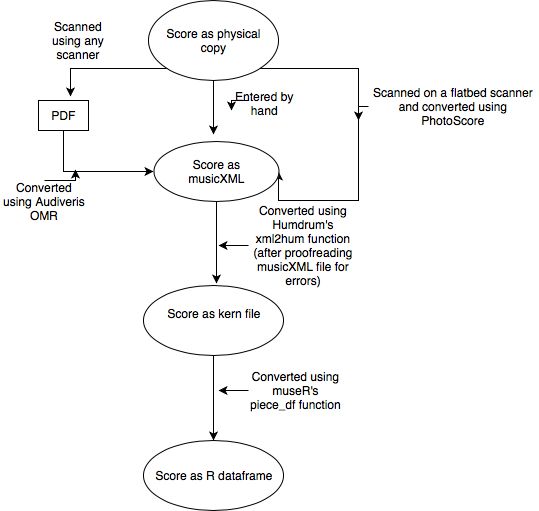
\includegraphics[scale = .5]{images/test.png}
\caption{Flowchart of the conversion process from physical copy to dataframe}
\label{subd}
\end{figure}
\section{Optical music recognition}\label{optical-music-recognition}

The vast majority of classical music is found solely in PDF or physical
copies. Sheet music as a form of data requires a lengthy process of
conversion before being able to be used in any analysis. Simply scanning
the scores into, say, a PDF, gives no musical semantics and can only be
viewed on screen or printed on paper. Thus, the two main steps in
reading in data from sheet music are: first using optical music
recognition software to transform physical scores into digital formats,
and second, to read the digital format in to R where subsequent analysis
can be done.
\begin{figure}[h]
\centering
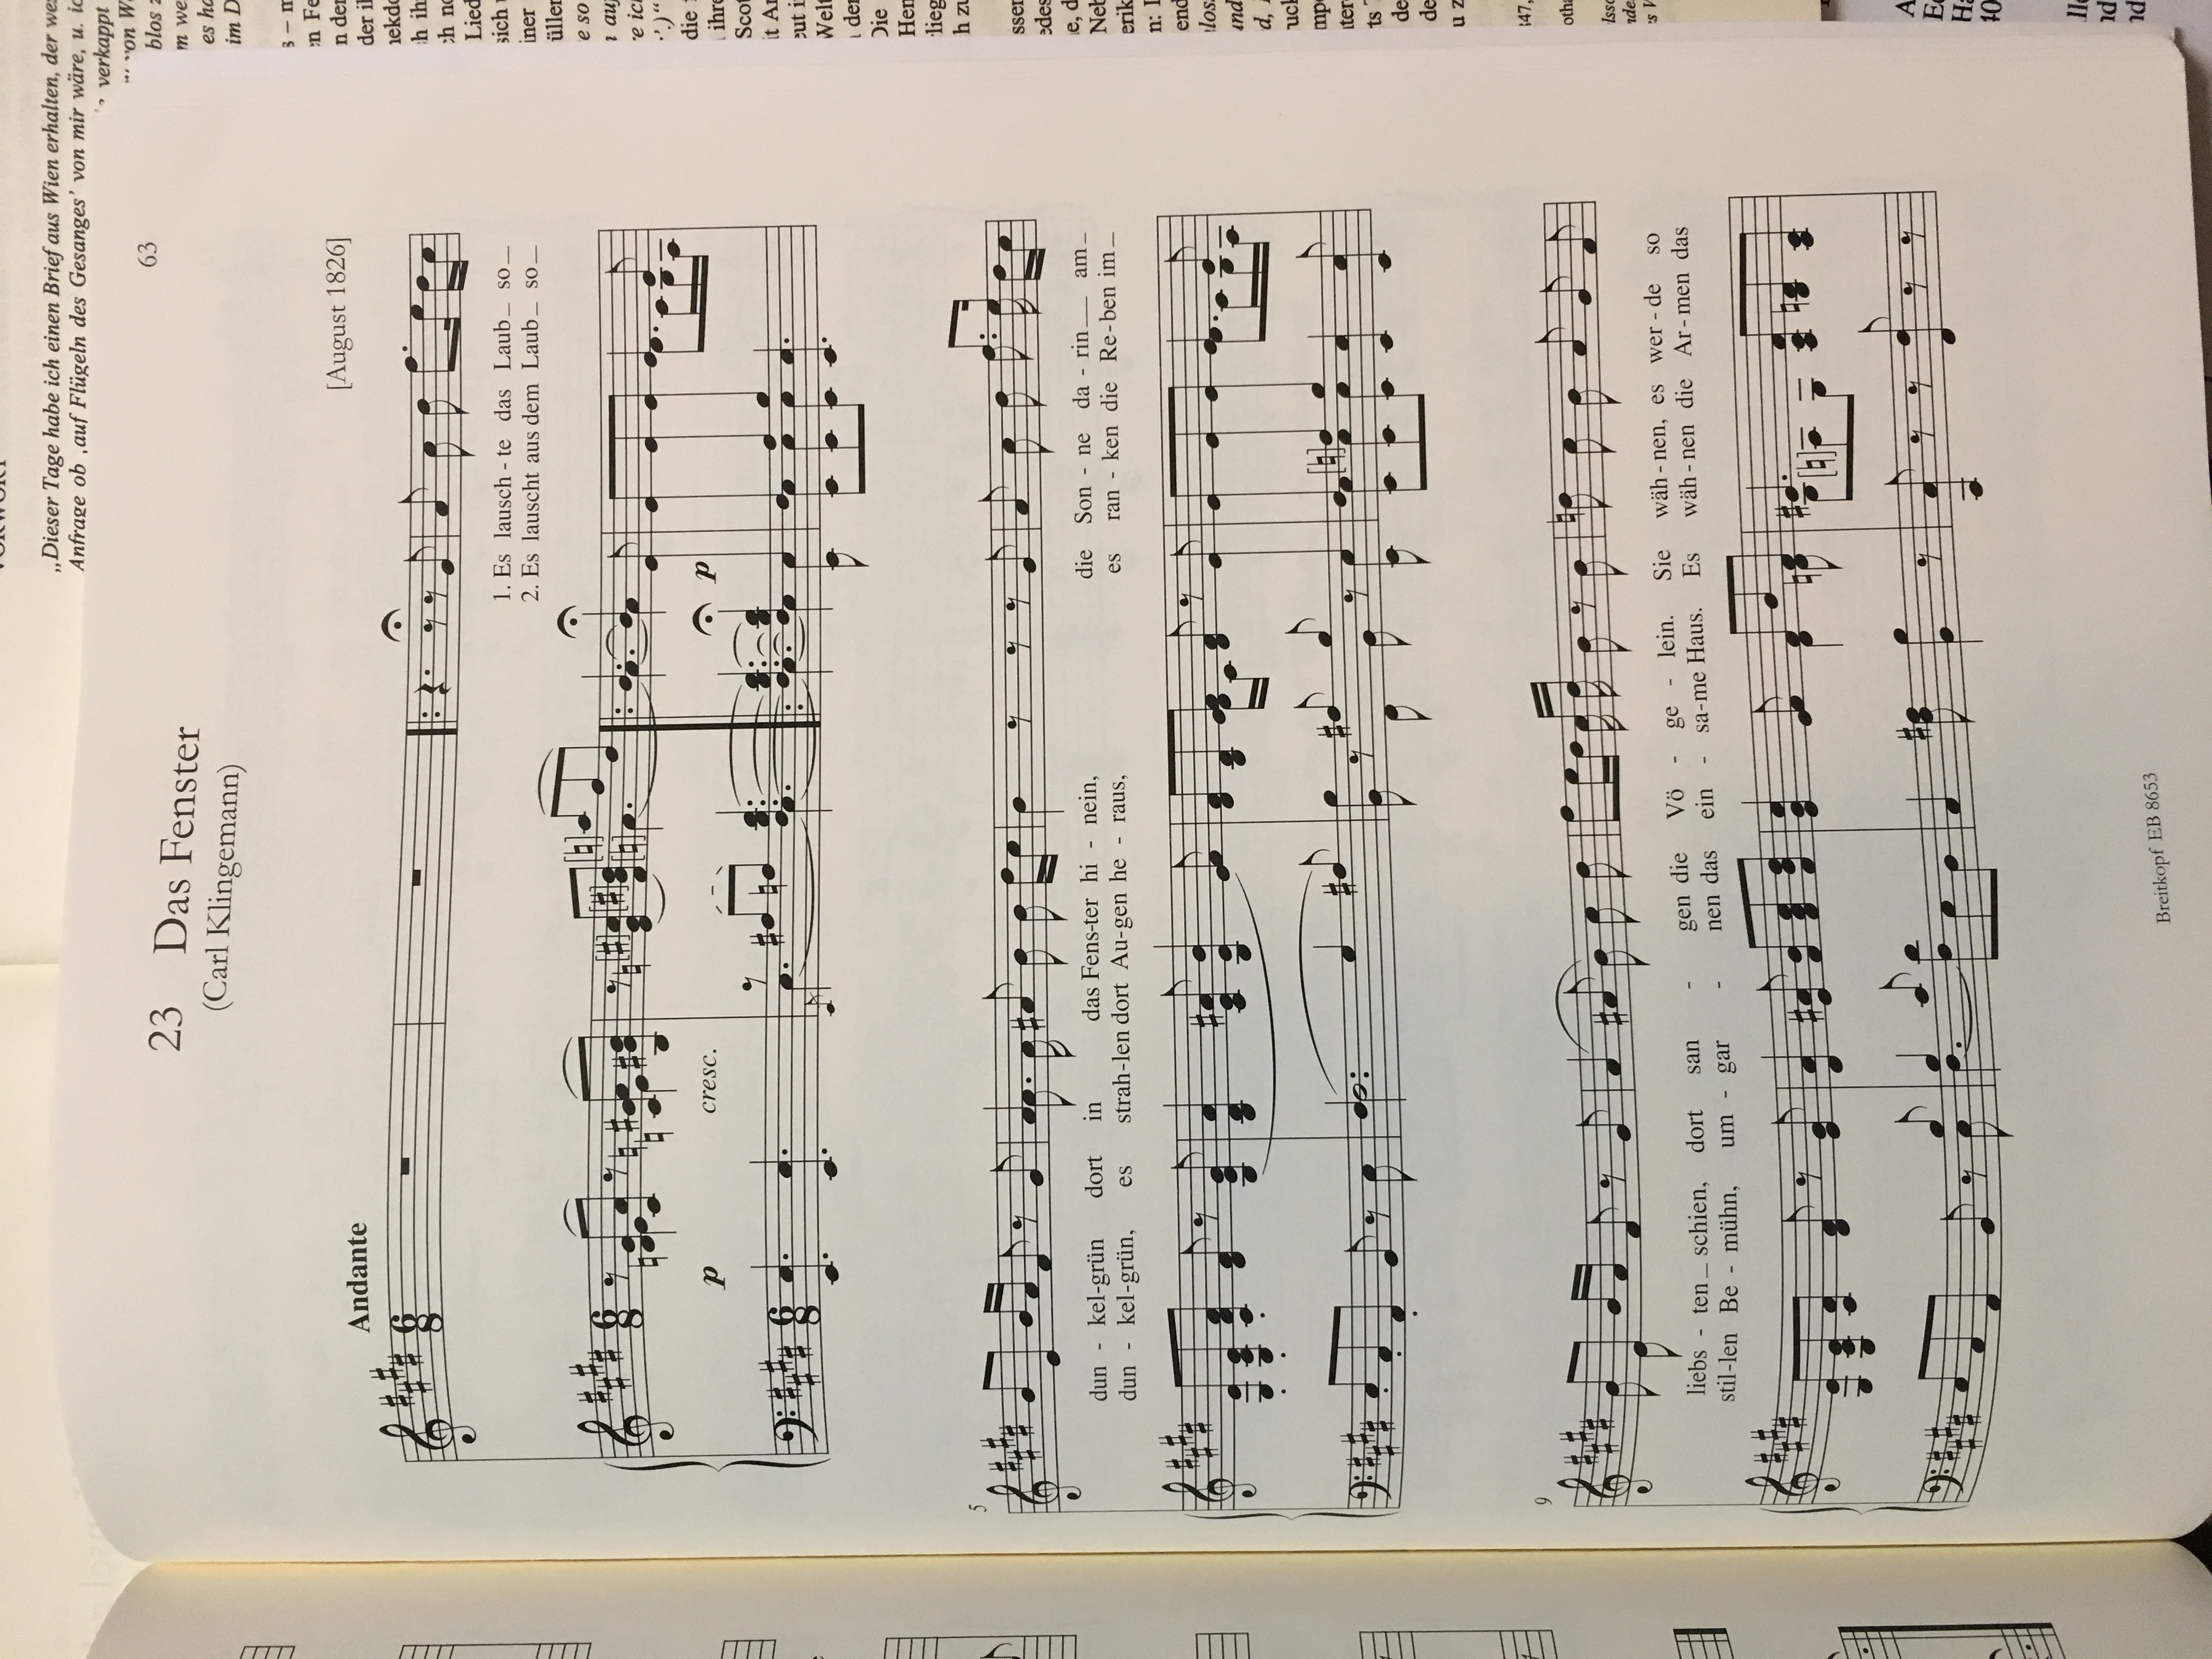
\includegraphics[scale=.50]{images/scorephoto.JPG}
\caption{Score in physical form before conversion process has started}
\label{subd}
\end{figure}
The scores used in this paper were obtained from physical copies
available in the Reed music library. These scores were then scanned
using software designed for optical music recognition (OMR).

Optical music recognition requires learning from graphical and textual
information. The main things the software must pick up are the locations
of bar lines, notes, rests, slurs, dynamic markings, tempo markings,
lyrics etc. Basic optical music recognition has been around since 1966.

Most commonly, the first step in optical music recognition is to remove
the staff lines. The staff lines are critical, as they define the basis
for the vertical definition distance of pitch, and the horizontal
distance definition of rhythm. The staff gives a normalization that is
helpful, essentially defining the size of what notes and rhythm look
like. Staff removal methods include projections, histograms, run
lengths, candidates assemblage, contour tracking, and graph path search.
(Doermann, Tombre, \& others, 2014)

The next step is music symbol extraction and classification. These
methods include template matching, where the object in question is
compared to existing known musical symbols, simple operators, such as
analysis of bounding boxes and projections, joining graphical
primitives, such as combining extracted objects such as notes, note
heads, and note beams to connect them in a musically correct way to form
chords etc. Other methods use statistical models for analyzing musical
primitives (the objects the OMR is trying to classify) such as Neural
Networks, Support Vector Machines, k-Nearest Neighbor, and Hidden Markov
Models.

The next step OMR performs is syntactical analysis and validation. This
step essentially uses defined grammars describing the organization of
music notation in terms of music symbols. This makes the classification
problem simpler, as there are existing rules and relationships between
musical symbols.

The two OMR softwares used in this paper were PhotoScore and Audiveris.
Each has its own benefits and issues. Photo Score works by scanning the
physical score on a flatbed scanner at a high resolution. It then uses
OMR techniques to output a musicXML file that can be read in by most
music composing software, such as Sibelius, Finale or Muse Score.

Audiveris in contrast works by inputting a high resolution PDF and then
uses OMR techniques to output a music XML file. Often, high enough
resolution PDFs do not exist, so the physical scores must also be
scanned by any garden variety scanner.
\begin{figure}[h]
\centering
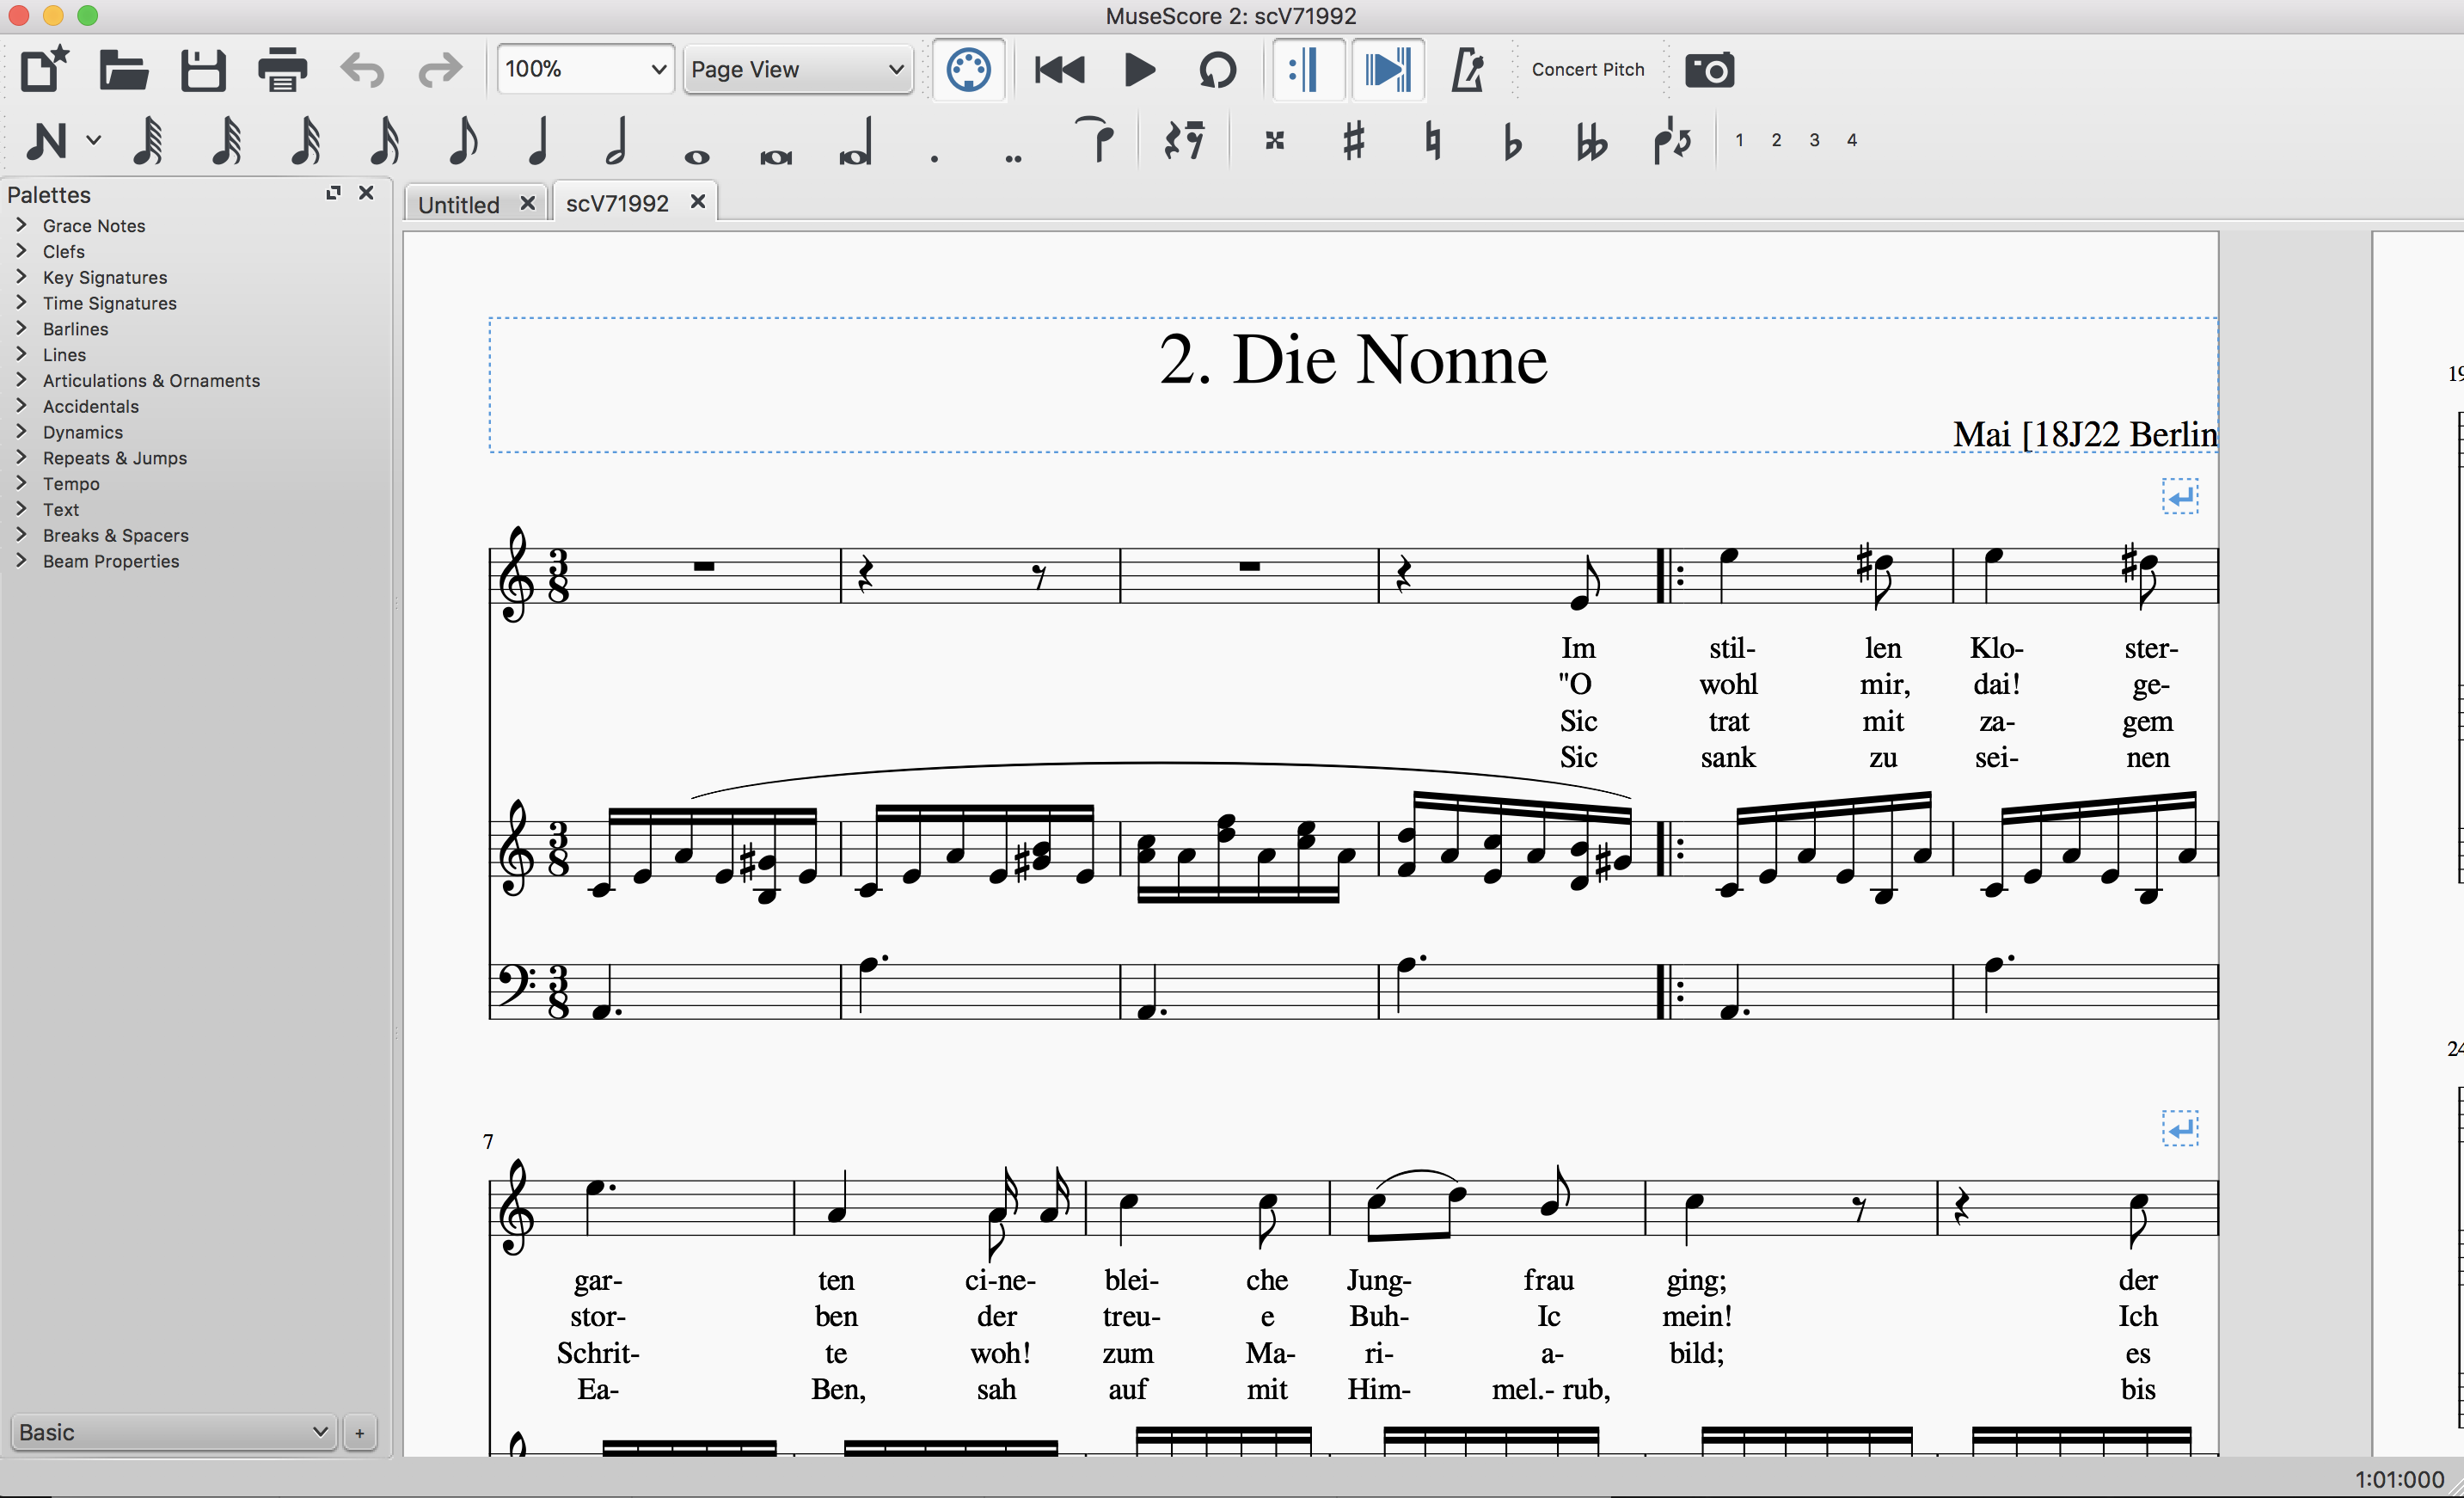
\includegraphics[scale=.30]{images/museScore.png}
\caption{A score in MuseScore format after being read by an OMR like PhotoScore or Audiveris}
\label{subd}
\end{figure}
MusicXML is commonly used as a format for digital music, as it is
conducive to representing sheet music and music notation, and it can be
transferable to many different music software. Muse Score was chosen to
be the music software for viewing digital scores, as it is a free
software that can read MusicXML.

After being scanned by PhotoScore and read into Muse Score, each piece
was proof-read and corrected. This involves looking through every piece
line by line for each bar to ``spell check'' the digital version.
PhotoScore did a good job recognizing notes, but often had issues
recognizing rhythms, and had issues keeping the structure of the piece.
Often in the scanning process clefs or bar lines were not found, causing
PhotoScore to output every staff on one line. Using PhotoScore, there
were on average approximately 6 minor issues per piece, although there
were on occasion major structural issues. Audiveris often added extra
beats to measures. It also always identified a bass clef as a baritone
clef.

Unfortunately, the scanning process is very lengthy and time consuming,
as the scanning often gives a large number of mistakes. Often the score
must be then scanned again. In addition the proof-reading process is
lengthy. One must check each note and theme for errors against the
original score, and change the afflicted notes using Muse Score. The
corrected score must then be output as a musicXML file. In addition,
there were some pieces that PhotoScore or Audiveris had a hard time
reading. These pieces were then entered into MuseScore by hand and then
proofread.

MusicXML on its own is not conducive to converting into a data frame as
representing the single half note middle C looks like this:
\begin{figure}[h]
\centering
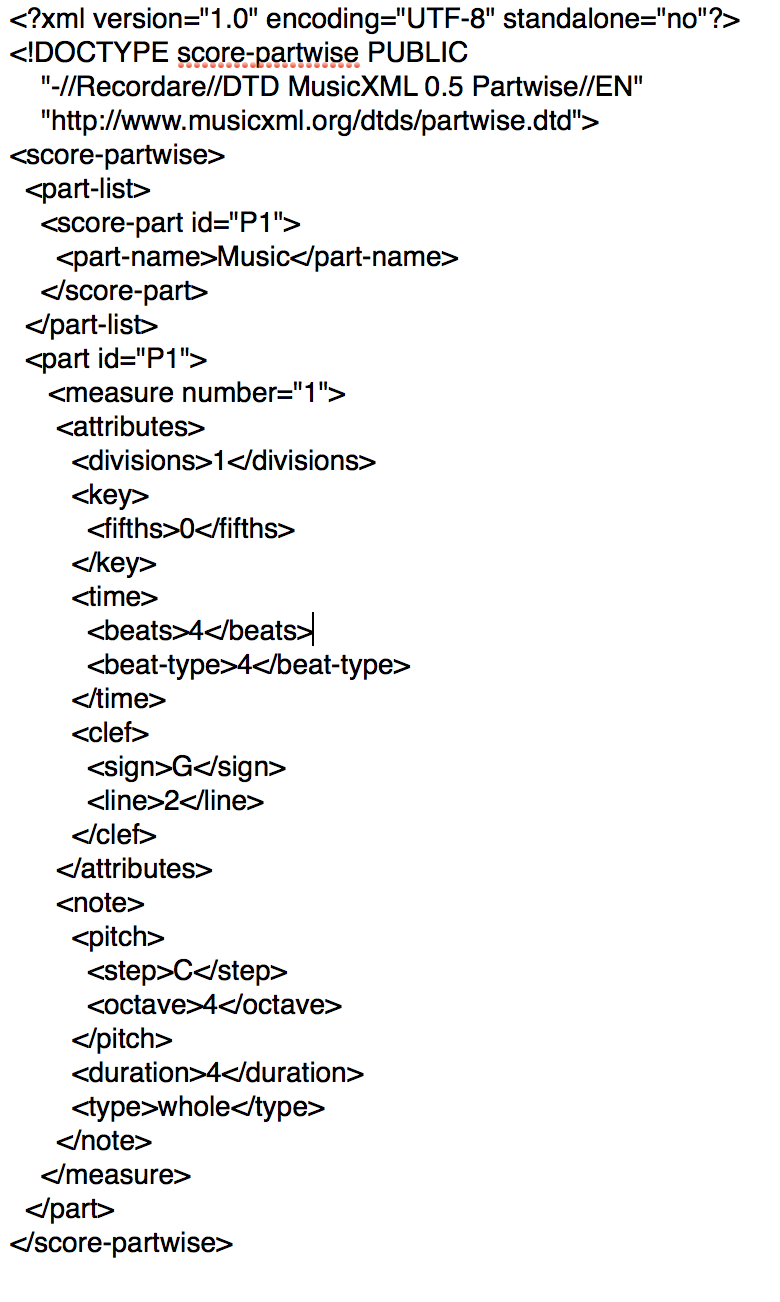
\includegraphics[scale=.30]{images/mxlc.png}
\caption{A half middle C in musicXML encoding}
\label{subd}
\end{figure}
We then need to convert into a format more easily readable into R. The
Kern Score music format is much more easily readable. It has clearly
expressed time signature, bar, beat and musical voicing information
(Mearns et al., 2010). Because of this, it is also more conducive to
being read into an R data frame. The below picture shows how a basic
piece of music corresponds to a .krn file.
\begin{figure}[h]
\centering
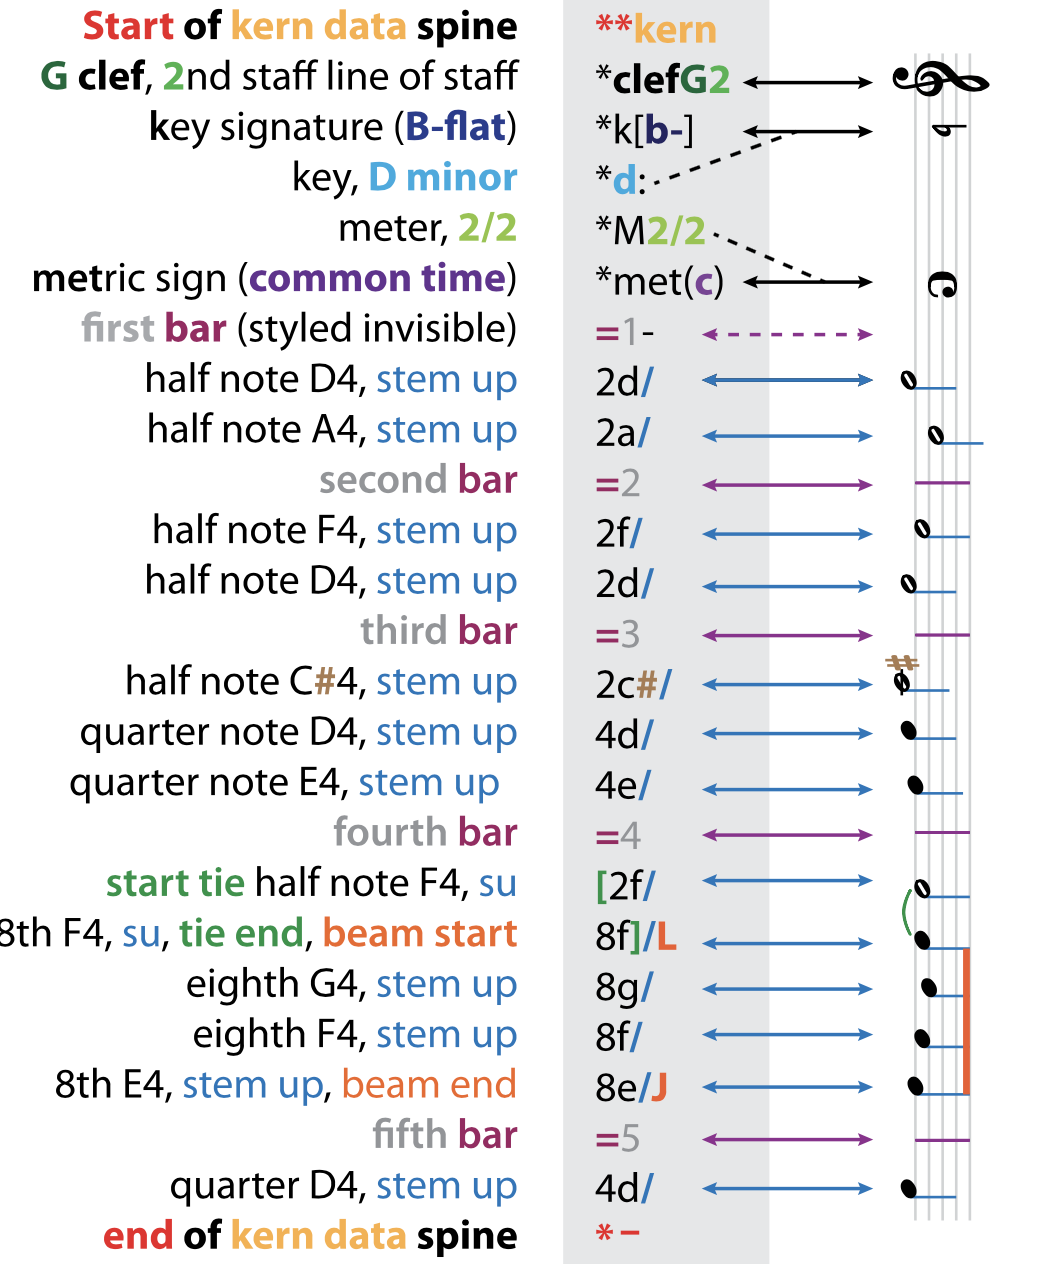
\includegraphics[scale=.50]{images/krnmusic.png}
\caption{How sheet music corresponds to kern files}
\label{subd}
\end{figure}
Kern files are organized with columns each representing one staff of
music. Each line of a Kern file represents one note of one value of a
time base. The time base for a Kern file is based on the smallest
(shortest) rhythm value of a note found in a piece. For example, if a
piece was in 4/4 and there were sixteenth notes present there would be
16*4 rows for each measure. The ``attack'' of each note is the only note
printed, the following time while the note is held is represented with
dots in the remaining rows until a new note is sounded for that staff.
The pitch of each note is represented by the letters a through g. The
case (lower or upper) as well as the repetition (c or ccc) represents
which octave the pitch occurs. Any accidental is represented with a \#,
-, or n symbol. Each instrument/staff in a piece is represented using
one (or more) columns called splines. For example, most lieder consist
of voice and piano. There are thus three splines, one for voice, one for
the treble clef staff of the piano, and one for the bass clef of the
piano. In addition, there are splines that contain the text for the
voice for the corresponding notes. This was not of interest to the
musical classification problem, so these splines were removed. Chords
are represented by multiple notes on the same line. For example, if
there was a half note C major triad followed by a quarter note D flat,
it would be represented as
\begin{verbatim}
2c 2e 2g
4d- . . 
\end{verbatim}
In addition, there is a lot of information about the appearance of the
piece, stem direction etc for notes, but this was decided as not
important for determining style, so it was removed.

We convert to kern format by using Humdrum's function \texttt{xml2hum}
that converts a musicXML file into a kern file. Humdrum is a
computational music software used to analyze music. It is a command line
tool that has many functions for music analysis. The Kern file type can
be read much more easily into R. Compared to above, the code for a
single middle c whole note would be :
\begin{verbatim}
**kern
*clefG2
*k[c]
*M4/4
=1-
1c/
\end{verbatim}
The import\_xml\_files.sh file goes through the process of converting
scores from musicXML to .krn. Each spline needs to to be individually
converted using xml2hum. The individual splines are then converted into
the same time base (there are issues when the bass line only has half
notes and the soprano line has a lot of 32nds). This conversion
essentially adds dots as placements so that the splines can line up
correctly by measure and beat.

The CCARH has a large data base containing work mostly Baroque and
Renaissance composers already in the Kern format, which is where the
Bach data came from.

The files that were scanned (ie all pieces by Felix and Fanny) need to
be separated into separate file for each staff, ie a seperate file for
each instrument. In addition, since we are focused on musical style, the
text of the pieces is removed in this stage. In the case of analyzing
lieder, each piece always has two or three files. These files consist of
voice, piano right hand, and piano left hand. This is necessary to avoid
the bugs in \texttt{xml2hum} that have issues when staffs don't
necessarily match up as a result of the conversion process. This is
often caused by an inconsistency in time base.

\section{.krn to R}\label{krn-to-r}

Once we have .krn files to represent each piece we use regular
expressions to extract key information. For scanned music (Felix and
Fanny music), there are as many files are there are staffs, usually
three. MuseR's \texttt{krn2df()} and \texttt{piece\_df()} functions read
in .krn files and output a data frame in R for each piece. First the
data in .krn format are read in line by line using R's
\texttt{readLines()} function. This takes every line of the .krn file
and converts it into a vector. Each entry contains the rhythem value and
note value for all notes in that line. If there are multiple notes
played at the same time, they are all in one line. The notes are
separated by splitting up the string by spaces. This converts a single
string representing one Kern line to multiple strings each representing
one note (or dot placeholder) for one Kern line. Then each entry is
separated out into the theme and note value for each note. Each line
contains the following columns: the measure the note occurs in, the
rhythm value for the note (for example 4), note name, octave inclusive
(for example cc), note name (octave exclusive){[} C sharp{]}. In
addition, for the whole piece the key signature and meter are recorded
as columns. If there are 3 splines and each spline has at most one note
at a time, there would thus be \(3 + 3*3=12\). If there are 3 splines
and one of the splines has at most 3 values, that is equivalent to
having 5 total splines there are then \$ 3 + 3*5 = 18\$ columns.

A lot of data included in the .krn files are not necessary. For example,
we assume that whether or not a note has a stem up or stem down offers
no help in classifying composer style, so this information is removed
when converting to an R data frame.

Inspired by the .krn file type, each row of the R data frame contains
one time base value. For a given piece, the time base represents the
shortest note duration value. For example, if the shortest note a piece
contained was a sixteenth note, the time base would be 16. Each measure
then would contain 16 rows. This results in many rows of NA for certain
instruments, when a note is still being voiced, but it is not the
instance of the note being attacked.

\chapter{MuseR and features}\label{muser-and-features}

To the best of my knowledge, there is currently no package of R that has
been built to analyze sheet music. There are existing packages (such as
tuneR) that examine audio formats of music. The intention of this thesis
was to create a package, museR, that imports sheet music in the proper
form (musicXML or Kern) and does all of the analysis using R.

\section{Importing data into R}\label{importing-data-into-r}

MuseR is equipped to import data in the Kern format. The functions for
converting these files are \texttt{kern2df()} and \texttt{piece\_df()}
These are most usefully in the form of individual splines. This allows
for naming the columns according to instrument. Below we have a short
piece appearing as it would look from MuseScore.
\begin{figure}[h]
\centering
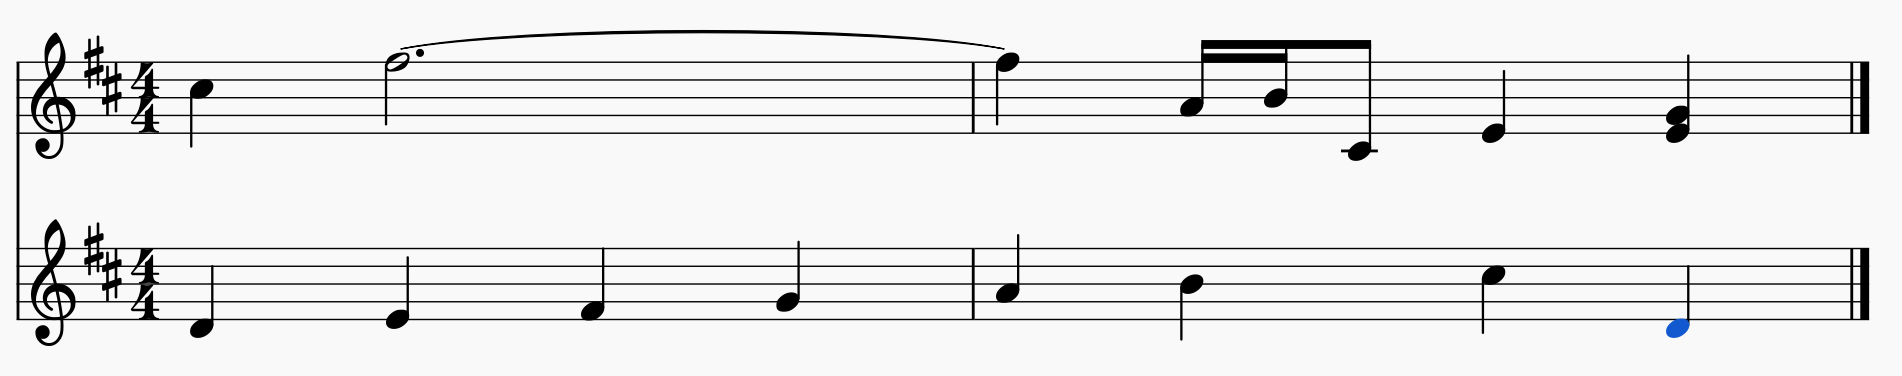
\includegraphics[scale = .5]{images/ex1m.png}
\caption{Example musescore format excerpt}
\label{subd}
\end{figure}
This piece would have the following Kern format representation:
\begin{figure}[h]
\centering
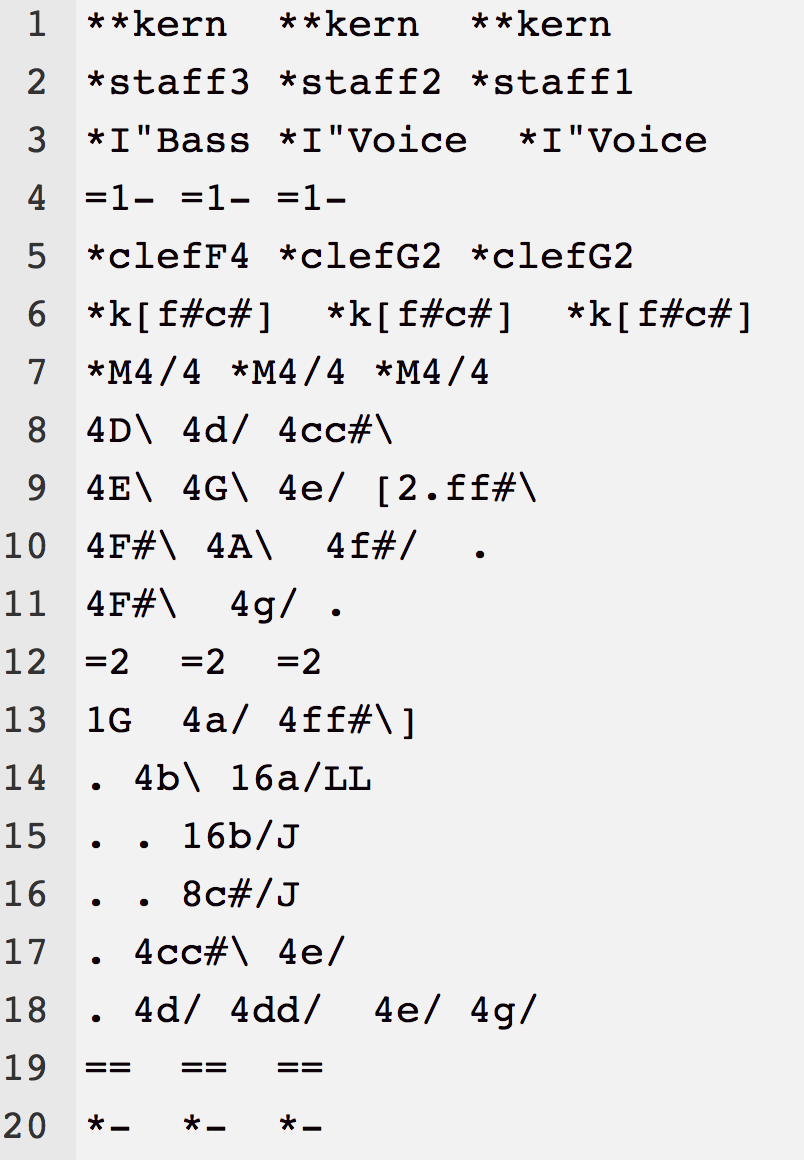
\includegraphics[scale = .5]{images/ex1k.png}
\caption{Example kern format excerpt of the above musescore}
\label{subd}
\end{figure}
Using museR's \texttt{piece\_df()} function to create the following data
frame.
\begin{figure}[h]
\centering
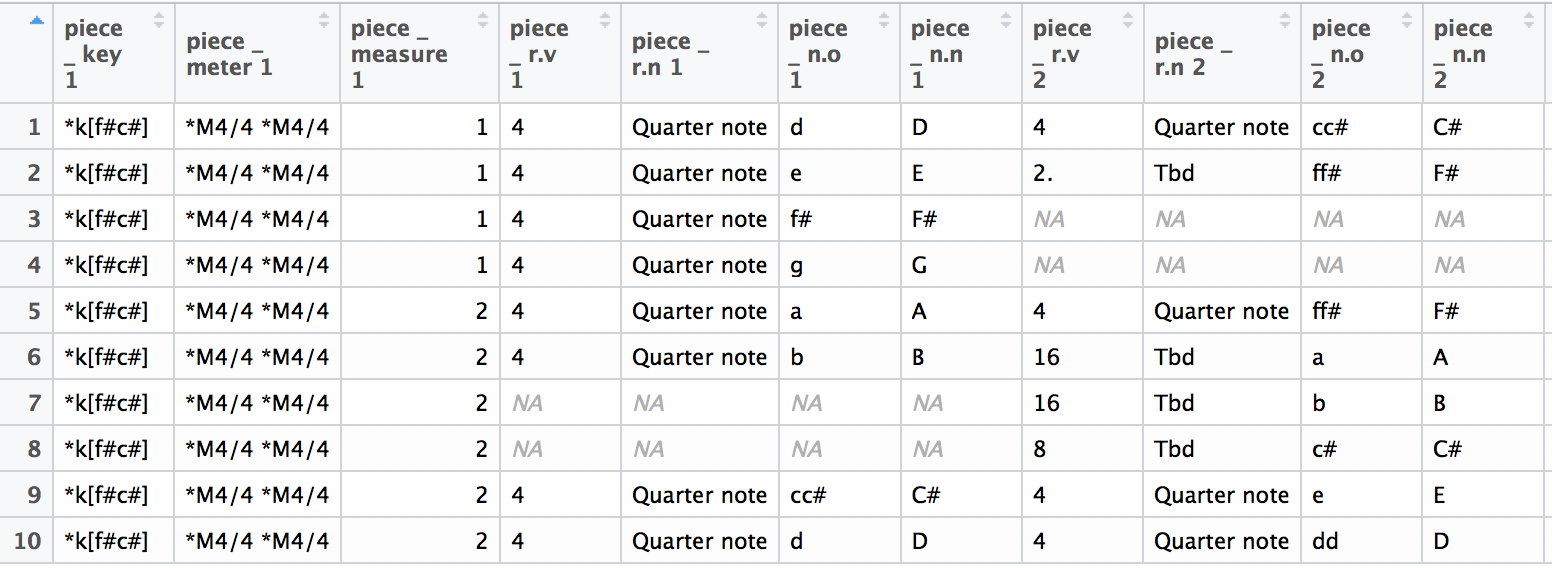
\includegraphics[scale = .5]{images/ex1r.png}
\caption{Example R data frame converted from the above MuseScore}
\label{subd}
\end{figure}
Data in R are commonly expressed as data frames. Expressing music as a
data frame has challenges, as music cannot be easily expressed in
rectangular form. Music as a data structure is very rugged. When
expressing it in rectangular form, there needs to be placeholder or
padding entries to account for the nonrectangularness. MuseR's
\texttt{piece\_df()} works by using regular expressions to extract note
and rhythem information. It uses NA and . values to indicate empty
spaces and duration respectively.

The output from \texttt{piece\_df()} follows the same ideas as the
structure of kern files. It has ``.'' values similar to the Kern dots
that represent the duration of the note for the timebase. This kind
structure is good for certain types of features, where we are intersted
only in the type of note happening, the time of the attack of the note,
or without considering rhythem. Sometimes, we are intersted in how long
the note lasts. The \texttt{durration\_df()} function corrects this
issue. It converts the \texttt{NA}s representing duration and replaces
them with the note value that is currently happening. This allows for
analysis that considers duration. The below figure represents the
durrational version of the above data frame.
\begin{figure}[h]
\centering
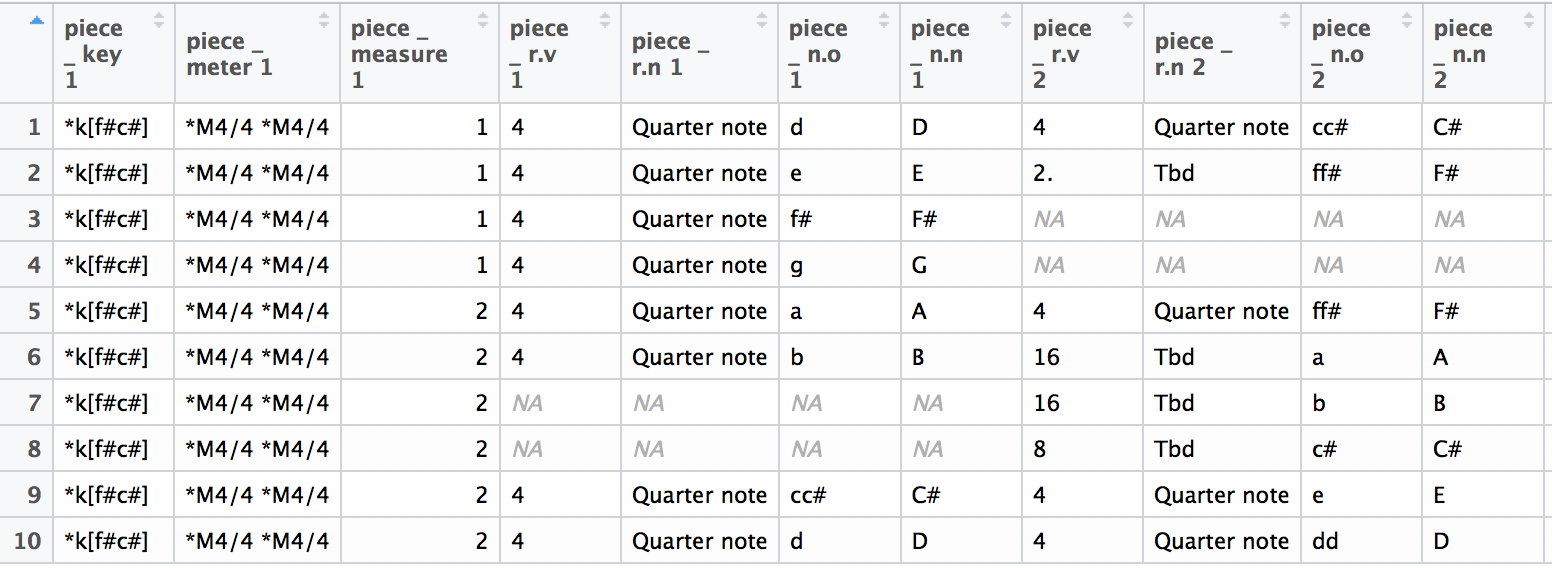
\includegraphics[scale = .5]{images/ex1r.png}
\caption{Example of durrationaly conveted data frame equivalent to the above data frame (need to change)}
\label{subd}
\end{figure}
\section{Features currently supported in
museR}\label{features-currently-supported-in-muser}

\subsubsection{Melodic intervals}\label{melodic-intervals}

Melodic intervals, or the interval between two successive notes, are
found using the \texttt{mel\_ints()} function. It is currently only
equipped to look at melodic intervals for the top note of each staff. In
this context, it is most commonely used for analyzing melodic intervals
of the voice. The function first extracts the top line of any
instrument, and then outputs the proportion of each melodic interval
happening over the whole piece. There are 12 possible intervals that are
counted (ignoring augmented and diminished):
unison,m2,M2,m3,M3,p4,tt,p5,m6,M6,m7,M7. \texttt{mel\_ints()} outputs a
vector of the proportion of each of the intervals.
\begin{figure}[h]
\centering
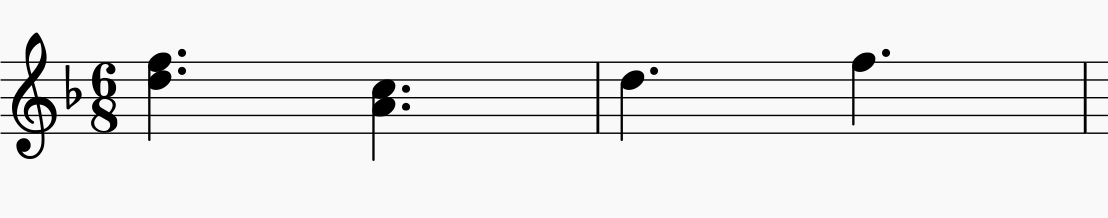
\includegraphics[scale = .5]{images/ex2.png}
\caption{Example of calculating proportion of melodic intervals}
\label{subd}
\end{figure}
For example if this function was run on the above piece, the melodic top
line intervals would be: \(\{(f,c),(c,d),(d,f)\} = \{p4,M2,m3\}\), which
would output the proportion vector \((0,1/3,1/3,0,0,1/3,0,0,0,0,0,0)\).

If we are interested in the types of melodic intervals, we can use the
\texttt{connsonance()} to examine the proportion of consonant (perfect,
imperfect, dissonant) intervals over the piece. This function works by
calling \texttt{mel\_ints()} and then adding up the perfect, imperfect,
and dissonant intervals proportions.

\subsubsection{Density}\label{density}

The \texttt{beat\_density()} function analysis the average and standard
devaition of density of each measure in the piece. It is called ``beat''
density as it only accounts for the instance a note starts. For example
if a measure consisted of a single whole note it would be only counted
once even though it is voiced the entire measure.

In the above example, the first measure would have a beat density of 4,
and the second measure woudl have a beat density of 2.

\subsubsection{Major\_minor}\label{major_minor}

For most musical analysis, the key of the piece is important in
determining chords, etc. The key is based on the key signature, which is
always given in a Kern file. Kern files from CCARH have the key of the
piece given, but scanned files do not. For kern files from CCARH,
\texttt{Major\_minor()} extracts the key given by the Kern file. for
scanned files, \texttt{Major\_minor()} identifies the two options for
key given the key signature. For example, if there was a key signature
with one sharp, the options would be G Major or E minor. The tonic for
each option is identified, and then the count of instances of both
choices for tonic is made. The key is determined by which of the options
for tonic has the higher count.

\subsubsection{Prop scale degree}\label{prop-scale-degree}

Once the key of a piece is determined, the proportion of each scale
degree is calculated. The scale degrees consist of : Tonic, Supertonic,
Mediant, Submediant, Dominant, Submediant, and Leading tone. In the
example above, if we assume the key is F major, the tonic has a tonic
scale degree proportion of 2/6, the mediant 1/6, dominant, 1/6,
submediant, 2/6.

\subsubsection{Chords}\label{chords}

Suspended chords are currently not supported by MuseR. Chords that
begin, or are ``attacked'' at the same time count.

First, the key of the piece is found, as different chords depend on the
key. Next, the times notes are played at the same time are extracted
into a list. Then the number of unique notes played at once is found. If
there are two notes played at once, \texttt{harm\_int()} calculates the
harmonic interval. This is done by calculating
\[note_1 - note_2 \mod(12)\] This gives the number of half steps between
each note. That number is then matched with the index of the interval.
Work is being done to have this include augmented and diminished
interval, but unfortunately that has not been completed at this time.

The possible triad chords are all defined by the intervals between each
note. For example, a Major triad is given by the base note, a major
third above the base, and a perfect fifth above the base. This
corresponds to 4 half steps then 4 half steps. Alternatively a minor
triad is given by the base, a minor third above, and a perfect fifth
above the base, which is 3 half steps, then 5 half steps.

A similar process is done for seventh chords.

\subsubsection{Length}\label{length}

We determine a measure for the length of a piece by how many measures
the piece has.

\subsection{Voice distance}\label{voice-distance}

The voice distance for each piece is measured as the range of the
singer, which is the distance in half steps between the lowest note the
singer sings and the hightest.

\section{Piano distance}\label{piano-distance}

Piano distance is the maximum distance between the lowest note in a
chord and the highest. Composers with different hand size could possibly
have different comfortable chords to play.

\chapter{About the Models}\label{about-the-models}

For classification, we are interested in using a set of features to
predict the response, or composer. The notation used in this chapter is
inspired by \emph{The Elements of Statistical Learning} (Friedman,
Hastie, \& Tibshirani, 2001) and \emph{An Introduction to Statistical
Learning} (James, Witten, Hastie, \& Tibshirani, 2013). Our features
space \(X\) is an \(n \times p\) matrix, where \(n\) is the size of our
data, and \(p\) is the number of predictors. Each \(X_i\) is vector of
values for a certain feature. \(x_{ij}\) denotes the \(i^{th}\) values
of the \(j^{th}\) feature. Each song has a composer or response, known
or unknown, denoted by \(Y\). In our case we have
\(Y \in \{\text{Fanny},\text{Felix}, \text{Bach}\}\), or more generally,
\(y \in \{\text{list of composers}\}\). The composer takes values in a
discrete set, which is the possible composers. Thus we can always divide
the input space into a collection of regions labeled according to the
classification

\subsection{Linear Methods for
Classification}\label{linear-methods-for-classification}

\subsection{Linear Regression:}\label{linear-regression}

A naive model for classification is linear regression. If our predictor
space \(Y\) has \(K\) classes, we code the response \(K\) different
indicator responses \(y_k\) where \(y_k = 1\) if \(Y = k\) and 0
otherwise. We can use the resulting \(k\) hyperplanes as a decision
boundary. We find the coefficients for the line by finding coefficients
\(\beta\) to minimize the residual sum of squares.

\[ RSS(\beta) = (\textbf{y} - \textbf{X}\beta)^T(\textbf{y} - \textbf{X}\beta) \]

where \(\textbf{X}\) is an \(N\times p\) matrix with each row an input
vector, and \(\textbf{y}\) is an \(N\)-vector of the outputs of the
training set. This gives the unique solution:

\[ \hat{\beta} = (\textbf{X}^T\textbf{X})^{-1}\textbf{X}^T\textbf{y}\]

This gives us;

\[\hat{\textbf{Y}} = \textbf{X}(\textbf{X}^T\textbf{X})^{-1}\textbf{X}^T
\textbf{Y}\] If there are \(K\) classes, and we have that the fitted
linear model for the \(kth\) class is
\(\hat{f}_k(x) = \hat{\beta}_{k0} + \hat{\beta}^T_kx\), the decision
boundary between class \(k\) and class \(l\) is the set of points for
which \(\hat{f}_k(x) = \hat{f}_l(x)\) which is equivalent to the set
\(\{x: (\hat{\beta}_{k0} - \hat{l0}) + (\hat{\beta}_k - \hat{\beta}_l)^Tx = 0\}\)
which is the hyperplane.

\subsubsection{Linear Discriminant
Analysis}\label{linear-discriminant-analysis}

Linear regression on a categorical variable that has multiple variables
has issues when there isn't a natural ordering with the categories. For
large \(K\) and small \(p\), groups can be masked. When there is a
binary response, we can calculate \(P(Y|X)\), but linear regression can
give predictions that aren't valid probabilities, namely negative
probabilities or probabilities greater than 1.

Knowing the class posteriors \(P(Y = k|X)\) gives us an optimal
classification. If we assume \(f_k(x)\) is the class-conditional density
of \(X\) in class \(G = k\) and that \(\pi_k\) is the prior probability
of class \(k\) with \(\sum_{k=1}^K \pi_k = 1\). We can then model
\(P(Y = k | X)\) by modeling the distribution of the features \(X\)
separately in each response class, and then use Bayes' theorem to
calculate \(P(Y = k |X)\) which gives us the following:

\[ P(Y = k | X = x) = \frac{f_k(x)\pi_k}{\sum_{l = 1}^Kf_l(x)\pi_l}\]

We thus must have a model to find \(f_k(x)\). Linear and quadratic
discriminant analysis assume a multivariate Gaussian density, given by:
\[f_k(x) = \frac{1}{(2\pi)^{p/2}|\mathbf{\Sigma}_k^{1/2}}e^{-\frac{1}{2}(x-\mu_k)^T\mathbf{\Sigma}_k^{-1}(x - \mu_k)}\]

Linear discriminant analysis (LDA) assumes that the covariance matrix is
equal for every \(k\):
\(\mathbf{\Sigma}_k = \mathbf{\Sigma} \forall k\). Quadratic
discriminant analysis does not have this assumption. In addition we
assume \(\hat{\pi}_k = N_k/N\) where \(N_k\) is the number of class -
\(k\) observations, \(\hat{\mu}_k = \sum_{g_i = k}x_i/N_k\), and
\(\mathbf{\hat{\Sigma}} = \sum_{k = 1}^{K}\sum_{g_i = k}(x_i - \hat \mu_k)(x_i - \hat\mu_k)^T / (N- K)\)

For LDA we can look at the log ratio comparing two classes \(k\) and
\(l\) and can show:

\[\log\frac{P(Y= k|x = x)}{P(Y = l|X = x)} = \log\frac{f_k(x)}{f_l(x)} + \log\frac{\pi_k}{\pi_l} = \log \frac{\pi_k}{\pi_l} - \frac{1}{2}(\mu_k + \mu_l)^T\mathbf{\Sigma}^{-1}(\mu_k- \mu_l) + x^T\mathbf{\Sigma}^{-1}(\mu_k - \mu_l) \]

This is a linear equation, so the classes will be separated by
hyperplanes. From the above, we can find that the predicted class for
any \(x\) is :

\[ \delta_k(x) = x^T\mathbf{\Sigma}^{-1}\mu_k - \frac{1}{2}\mu_k^T\mathbf{\Sigma}^{-1}\mu_k + \log \pi_k \]

These functions are known as \(\textit{linear discriminant functions}\)
We predict the class by finding the maximum value of the discriminant
functions of all \(k\).

For QDA we get the following discriminant functions:
\[ \delta_k(x) = -\frac{1}{2}\log|\mathbf{\Sigma}_k| - \frac{1}{2}(x - \mu_k)^T\mathbf{\Sigma}_k^{-1}(x - \mu_k) + \log \pi_k \]

Linear discriminant analysis is helpful when the classes are well
separated, when \(n\) is small and the distribution of the predictors
\(X\) is approximately normal in each of the classes, and when there are
more than two response classes.

\subsubsection{Naive Bayes}\label{naive-bayes}

The Naive Bayes classifier is often used for musical classification as
it is good when the dimension \(p\) of the features space is large. It
makes the (naive) assumption that all the features are independent for a
given class \(i\), ie that \[f_i(X) = \prod_{k = 1}^p f_{ik}(X_k)\]. In
practice this is not the case, but the model still preforms surprisingly
well in practice when this assumption does not hold.

\subsubsection{Logistic Regression}\label{logistic-regression}

Logistic regression differs from linear discriminant analysis by
directly modeling \(P(Y = k|X)\) by using the logistic function. The
idea is to model the posterior probabilities of each of the \(K\)
classes as linear functions in \(x\) and requiring that the
probabilities sum to 1. The model has the form:
\[ \log \bigg( \frac{p(X)}{1-p(X)} \bigg) = \beta_0 + \beta_1 X_1 + \cdots + \beta_pX_p\]

which can be written as:

\[ p(X) = \frac{e^{\beta_0 + \beta_1X_1 + \cdots + \beta_pX_p}}{1 +e^{\beta_0 + \beta_1X_1 + \cdots + \beta_pX_p} }\]

We estimate the regression coefficients by using maximum likelihood. The
log-likelihood for \(N\) observations is:

\[ \ell(\theta) = \sum_{i = 1}^N \log p_{g_i}(x_i;\theta)\] where
\(p_k(x_i;\theta) = P(Y = k|X = x_i;\theta)\) We then choose \(\theta\)
to maximize this function.

\subsubsection{K- nearest - neighbor
(expand)}\label{k--nearest---neighbor-expand}

Another method for classification is k-nearest neighbor methods. It uses
observations in the training set closest to \(x\) to form \(\hat{Y}\),
the outputs. We often use Euclidean distance as a metric for closeness,
although other methods exist. It is defined as
\[ \hat{Y}(x) = \frac{1}{k}\sum_{x_i \in N_k(x)}y_i\]

where \(N_k(x)\) is the \(k\) closest points, or neighbors, \(x_i\) in
the training set. This is equivalent to taking the average of \(k\)
observations with \(x_i\) closest to \(x\). This gives a predicted class
of taking the mode of the \(k\) nearest neighbors.

\subsection{Dimensionality Reduction}\label{dimensionality-reduction}

\subsubsection{Principal component
analysis}\label{principal-component-analysis}

Principal component analysis (PCA) tranforms the features space into a
lower dimensional representation. It choses the transformed features to
have maximal variance and be mutually uncorrelated.

Principal component analysis can be useful when the predictors are
correlated. We suspect many of our features are correlated, due to
certain patterns in music, as well as the way we created our features.
These relationships are caused by similarity in the features, and from
music theory rules. (For example, if there is a high frequency of first
scale degrees, we might expect a high frequency of chords that include
the first scale degree. Another example, if we had a high frequency of
seventh scale degrees, we would expect them to resolve to the first
scale degree.)

Principal component analysis is also helpful when there are many
predictors, and we want to deal with a smaller dimension of predictor
space.

As an unsupervised method, PCA can inform about latent meta variables.

Used in supervised methods, the transformed features from PCA can be
used to fit models instead of the original features space.

Principal components transforms the feature space. If our original
features are \(X_1,X_2,\ldots,X_p\), we transform the features to
\(Z_1,Z_2,\ldots,Z_M\), where \(M < p\). Each \(Z_i\) is a linear
combination of the original predictors, ie,
\(Z_m = \sum_{j = 1}^p \phi_{jm}X_j\), for constants
\(\phi_{1m},\phi_{2m},\ldots,\phi_{pm}\) for \(m = 1,\ldots,M\). Given
an \(n\times p\) data set \(\mathbf{X}\) where \(x_{ij}\) is the
\(i^{th}\) instance of the \(j^{th}\) feature, we solve for the
\(m^{th}\) principal component loading vector
\(\phi_m = \phi_{1m},\phi_{2m},\ldots,\phi_{pm}\) that solves the
optimization problem:
\[\max_{\phi_{1m},\ldots,\phi_{pm}} \bigg\{\frac{1}{n}\sum_{i=1}^n\bigg(\sum_{j=1}^p \phi_{jm}x_{ij}\bigg)^2\bigg\}\],
where the \(\phi\)s are subject to \(\sum_{j = 1}^p\phi_{jm}^2 = 1\).
Our principal components are then calculated as
\(z_{im} = \sum_{j = 1}^p\phi{jm}x_{ij}\)

The loadings of the first principal component, \(\phi_1\) thus determine
the direction in the feature space with the most variance, \(Z_1\), or
the scores of the first principal component is then a new feature in our
transformed feature space. We continue calculating \(Z_i\), where each
following \(Z_i\) has the maximal variance in a direction uncorrelated
to the previous principal components.

Before PCA is performed, we center all features to have mean zero, as
the scale of some features are not the same, which will lead to issues
in the loadings, as the features with higher scales would automatically
have the higher variance.

We can observe the proportion of variance explained by each principal
component. This is usually visualized in a skree plot. We can use this
information to decide how many principal components to use.

\subsection{Model selection/assesment}\label{model-selectionassesment}

\subsubsection{5-fold Cross validation
(expand)}\label{fold-cross-validation-expand}

Cross validation involves fitting a model on a training set, and then
using the fitted model to predict the responses in the testing set.
\(k\)-fold cross validation involves splitting the data set into \(k\)
different parts of equal size, and fitting a model on the the data set
with one of the \(k\) parts withheld. The model is then tested on the
witheld data. This is useful for model selection and determining the
accuracy of the model. In this paper, as is common, we use \(k = 5\)

\subsection{Lasso model selection}\label{lasso-model-selection}

The Lasso penalty was proposed by Robert Tibshirani in 1996. Lasso
regression works by giving a penalty to regression coefficients. It
essentially performes variable selection, as for high enough penalties,
coeficcients shrink to zero. It is often used in linear regression, but
can be expended to logistic regression and other generalized linear
models. For linear regression, the lasso works by choosing coefficients
\(\beta_\lambda^L\) that minimize
\[ \sum_{i = 1}^n \bigg( y_i - \beta_0 - \sum_{j = 1}^p \beta_jx_{ij}\bigg)^2 + \lambda \sum_{j = 1}^p|\beta_j|\]
We have that \(\lambda\) is a tuning parameter. Increasing \(\lambda\)
will shrink the coefficients. This can be equivantely stated as:
\[ \text{minimize}_\beta \bigg\{\sum_{i = 1}^n\bigg(y_i - \beta_0 - \sum_{j = 1}^p \beta_jx_{ij}\bigg) ^2 \text{ subject to } \sum_{j = 1}^p |\beta_j| \leq s\]

To expand to generalized linear models, if our model uses some parameter
\(\beta\) that was estimated by by some function \(\ell(\beta)\) (where
\(\ell(\beta)\) is a log-likelyhood function for example), we maximize
\(\ell(\beta)\) subject to \(\sum_{j=1}^p|\beta_j| < s\) (Tibshirani,
1996)

\subsection{Some trees?}\label{some-trees}

\subsection{K-Measns Clustering (plus other
clusterings?)}\label{k-measns-clustering-plus-other-clusterings}

\chapter{Exploratory Data Analysis}\label{exploratory-data-analysis}

\section{Bach and Mendelssohns}\label{bach-and-mendelssohns}

Below (will be?) the pairwise distributions of each of the features used
for Bach and the Mendelssohn s. There are higher correlations between
scale degree frequencies 3 and 6. There is also a surprising separation
between the composers for the mean density.
\begin{figure}[h]
\centering
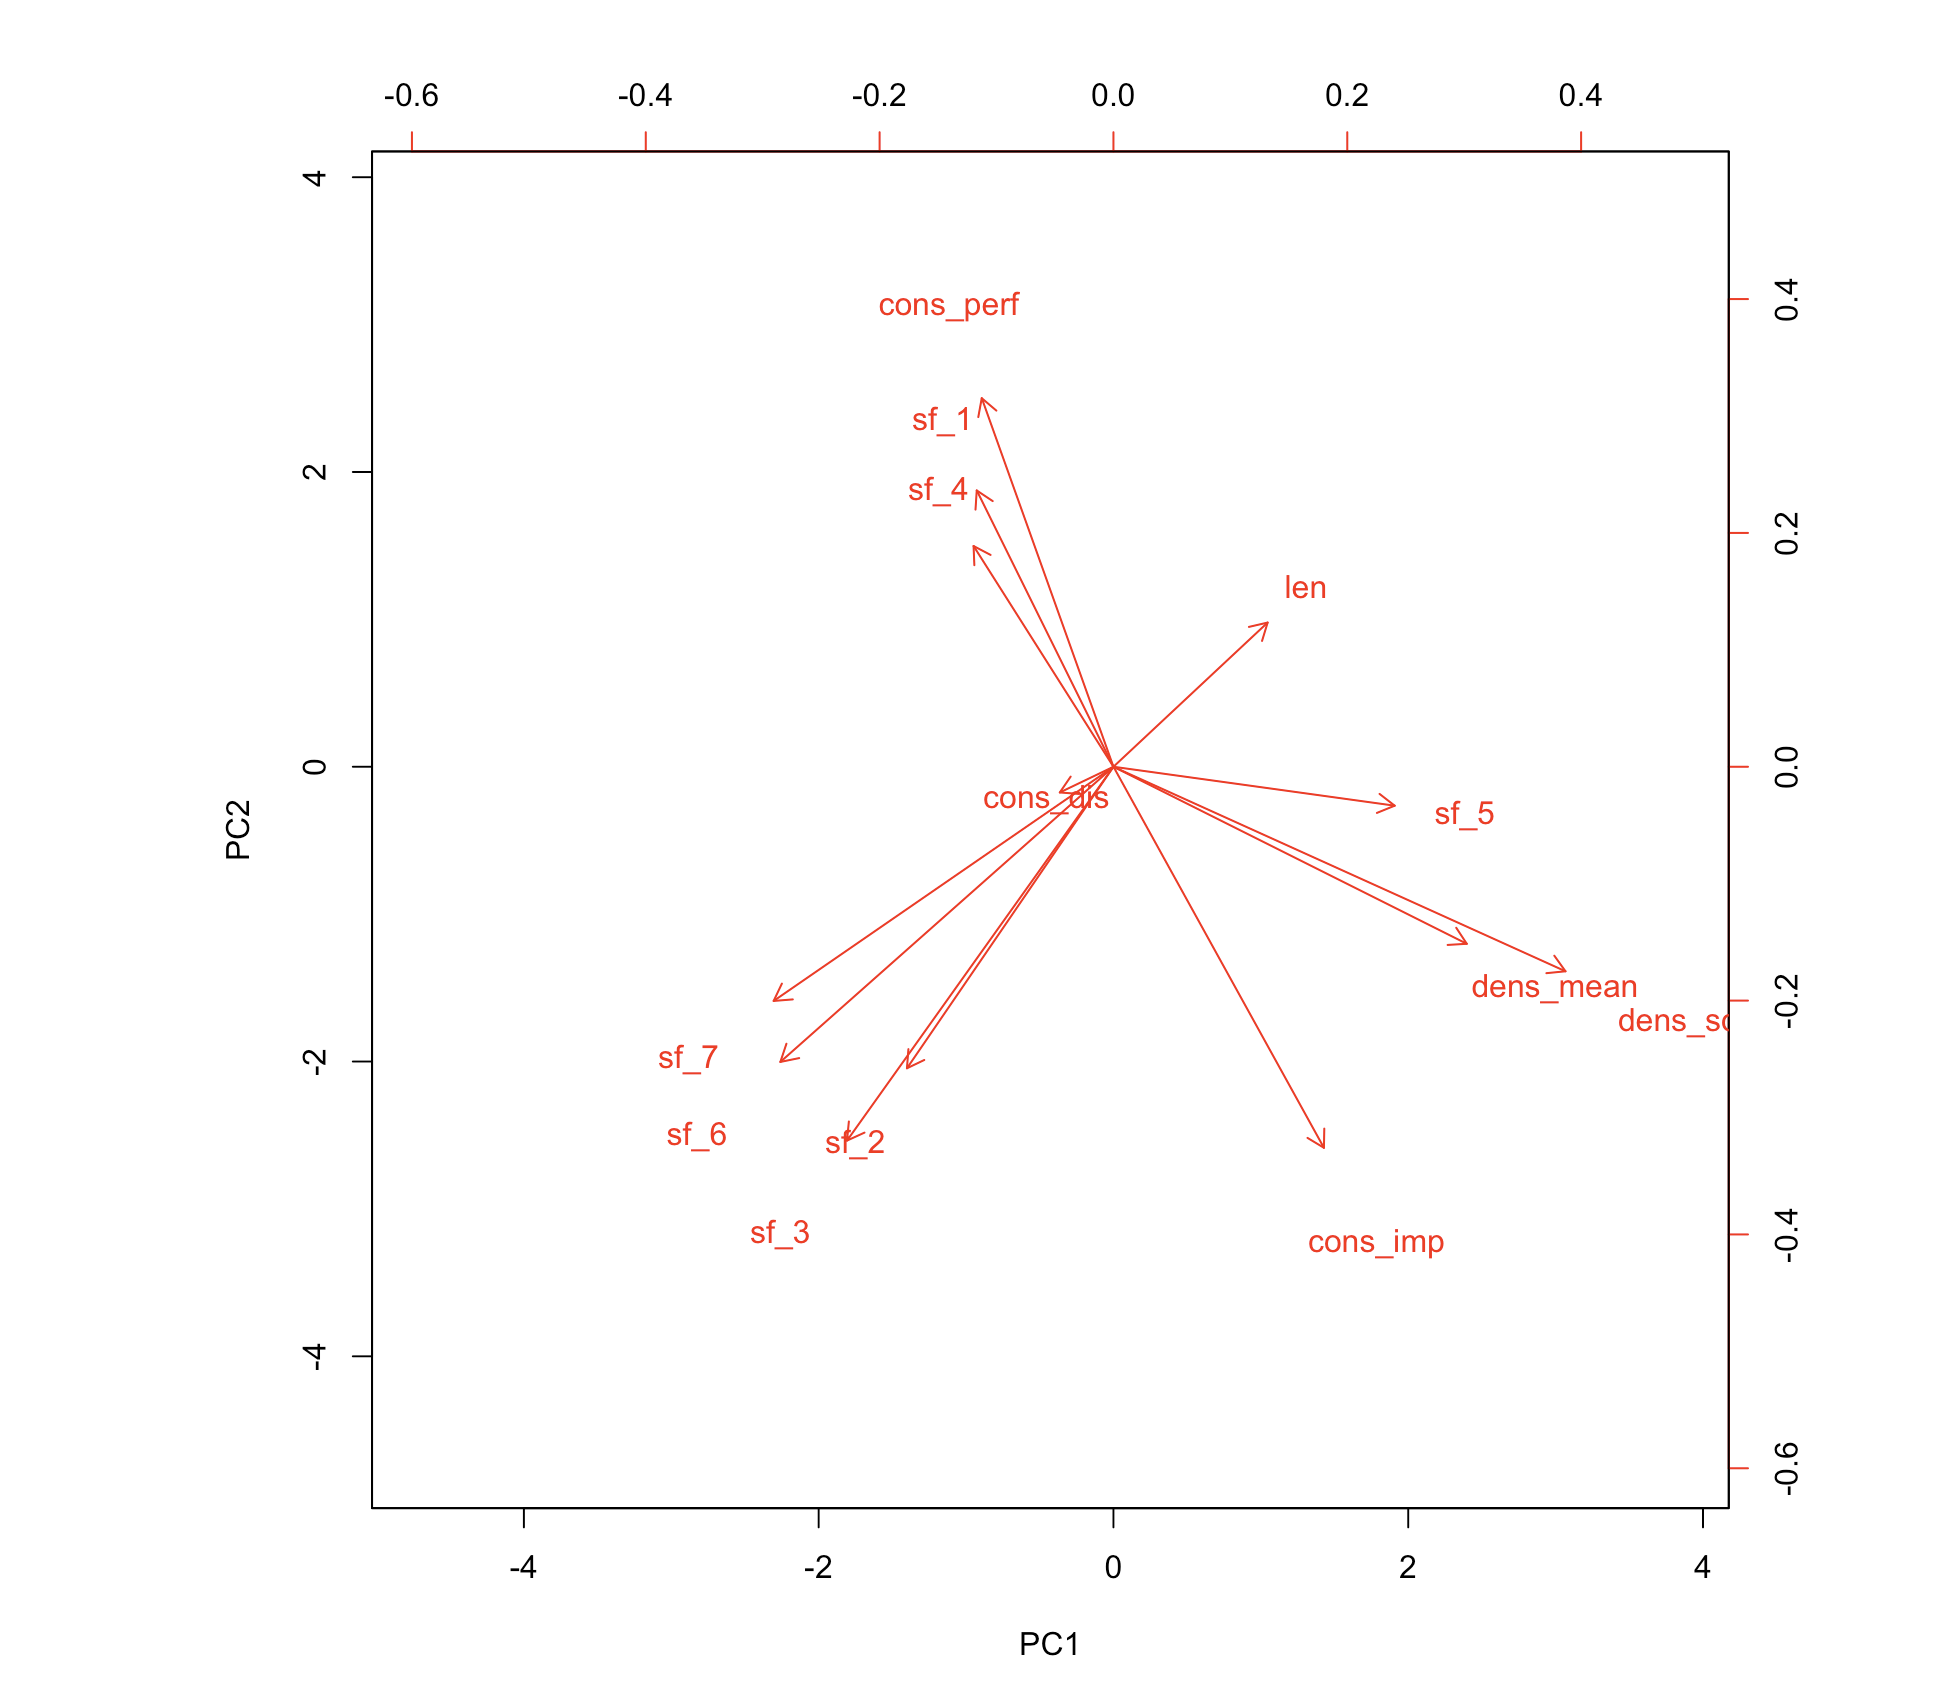
\includegraphics[scale = .3]{images/n_label_bi_bm.png}
\caption{Biplot of the loading vectors of the first two principal components}
\label{subd}
\end{figure}
The above biplot shows the loading vectors plotted on the first two
principal components. The loading vectors of features seem to arrange
into aproximately three groups. The features: perfect consonances of
melodic intervals of the voice, frequency of the first scale degree,
frequency of the fourth scale degree are all grouped together.
Similarly, frequencies for the 7th, 6th, 2nd, and 3rd are grouped
together. In addition we have perfect consonances and imperfect
consonances on two sides of the second principal component. This leads
me to believe that the second principal component encodes some sense of
use of consonant notes. The first principal does not seem to have a
musical interpretation. (I think?)
\begin{figure}[h]
\centering
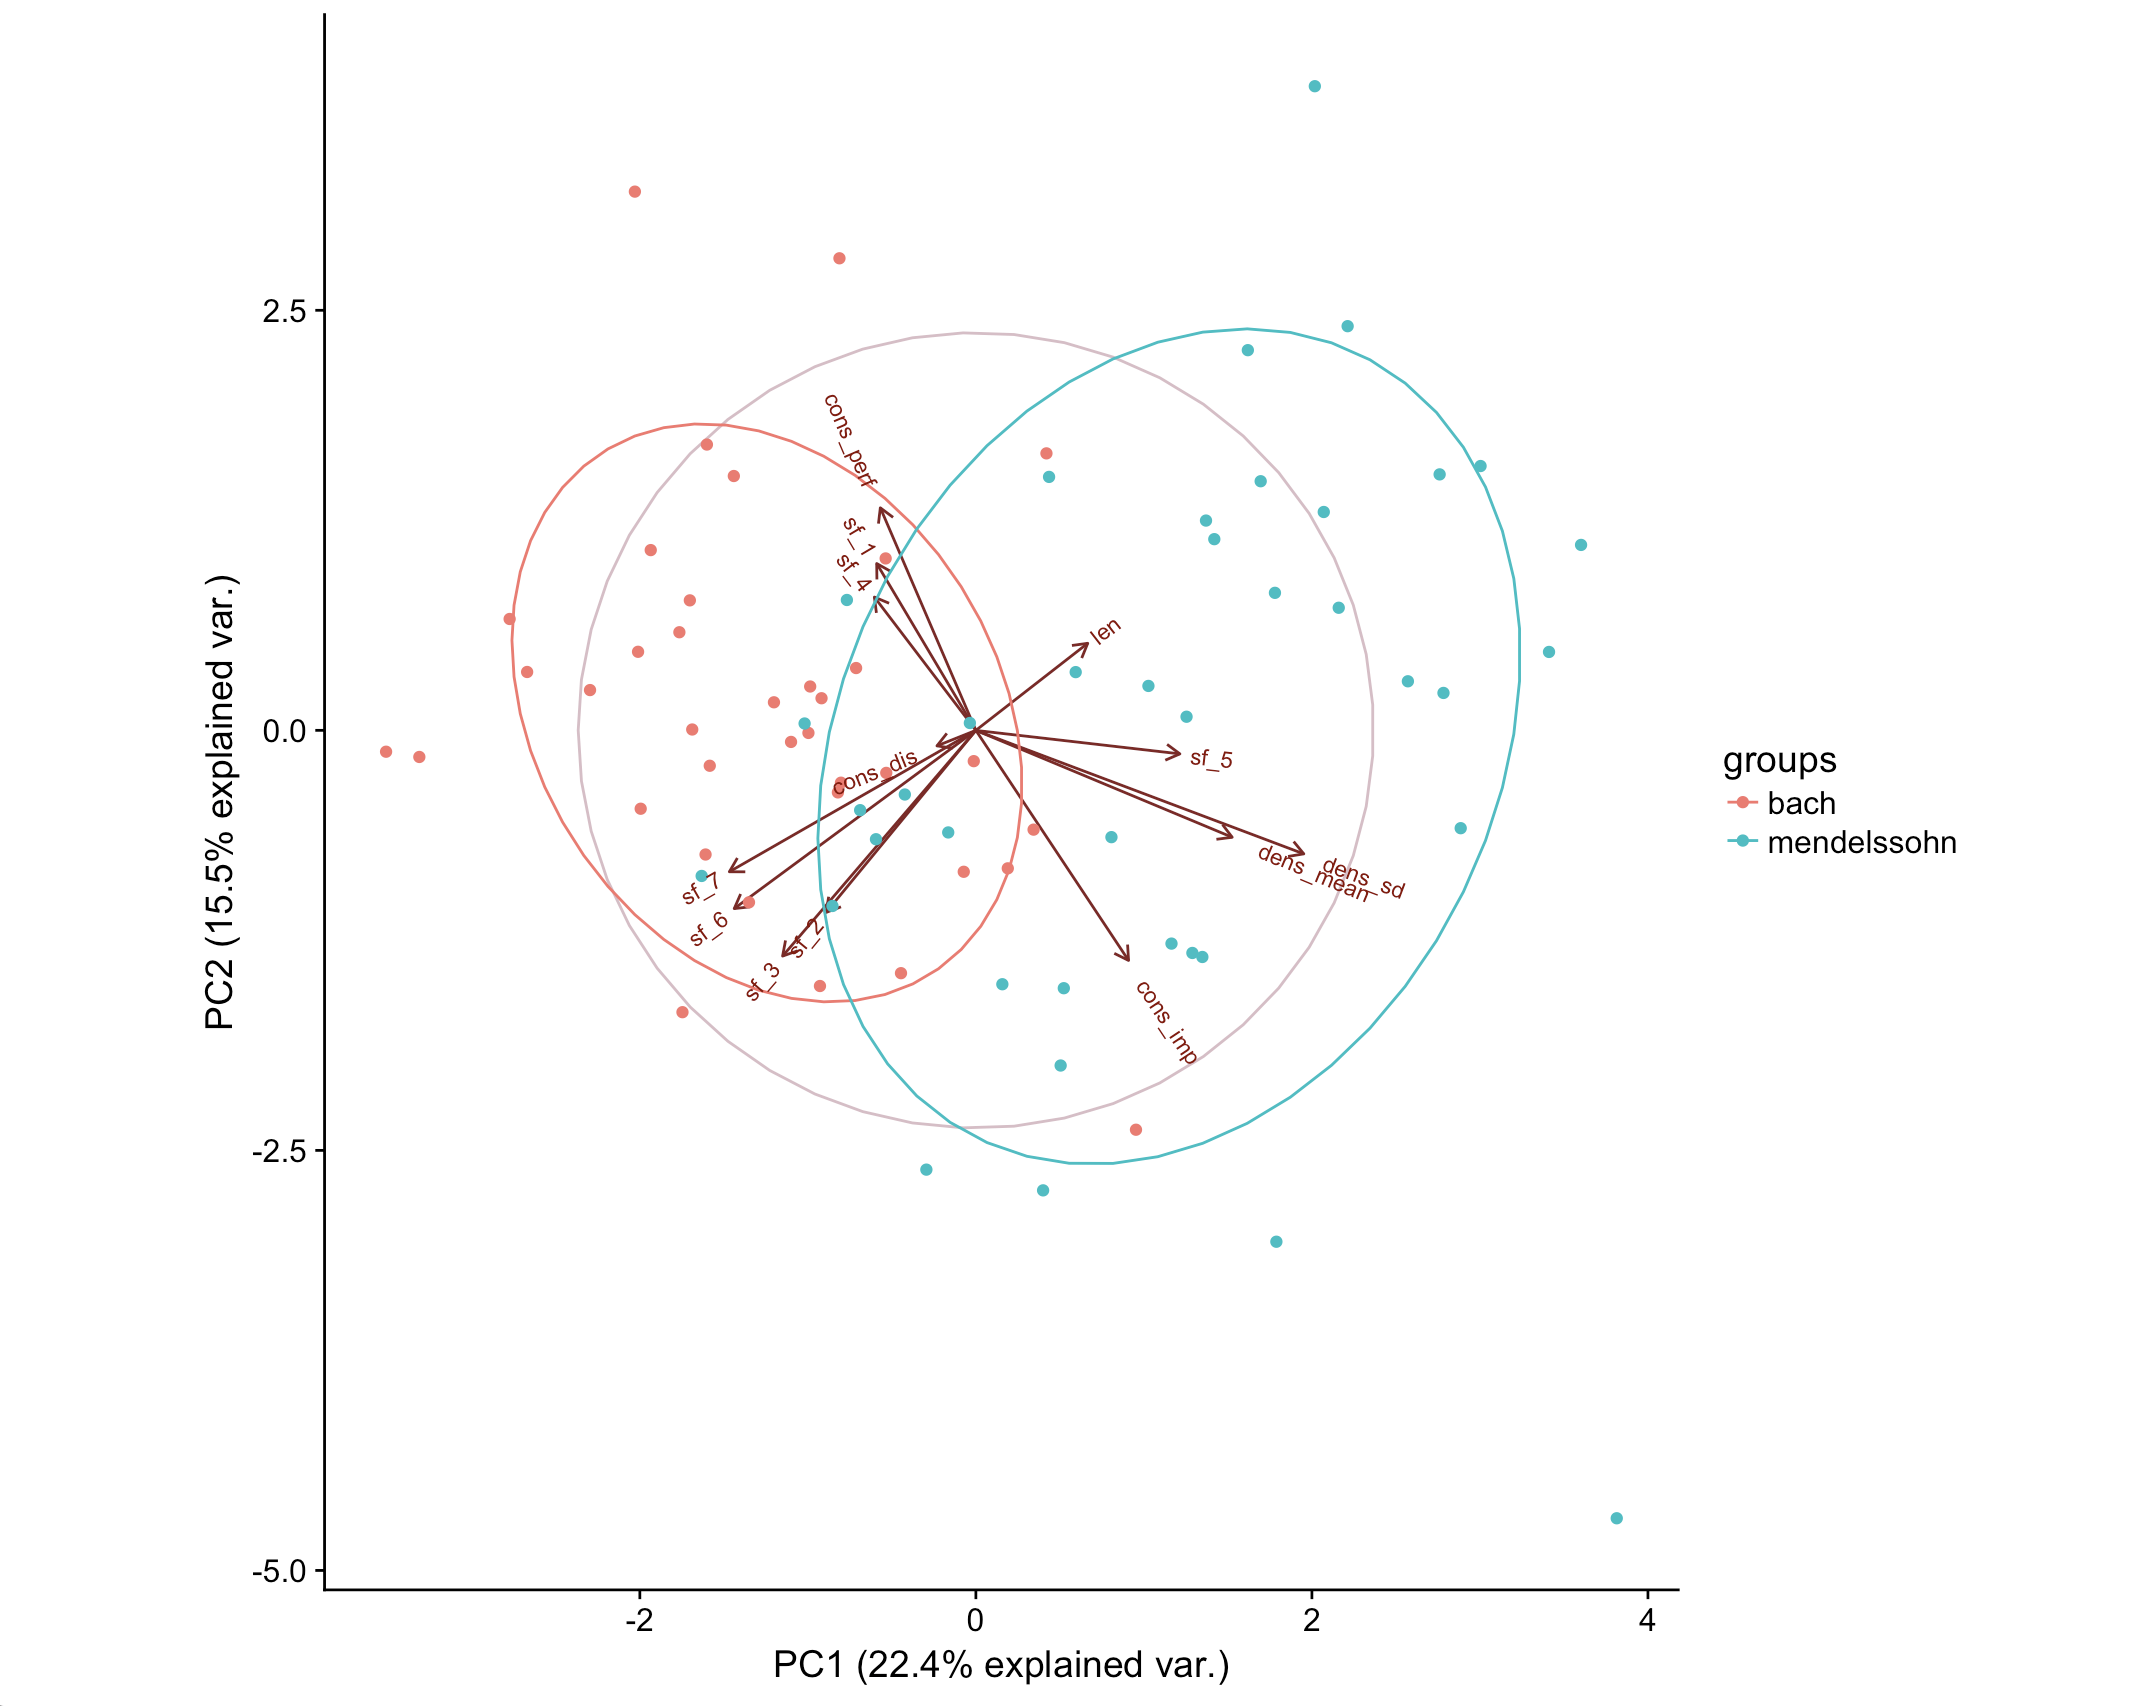
\includegraphics[scale = .3]{images/circle_bf_biplot.png}
\caption{Biplot of the first two principal components plotted with data points colored by composer. }
\label{subd}
\end{figure}
The above? plot shows the same prinicpal components, with the addition
of points representing each piece graphed by their first two principal
components. The elipses represent a \ldots{}.. The pieces are colored by
thier composer. There does seem to be a decent amount of seperation
between the groups, although it is not complete. The below plot shows
the pieces plotted on the second and third principal compenent, and
there is much less seperation. Also there does not seem to be an obvious
musical interpretation of the loadings.
\begin{figure}[h]
\centering
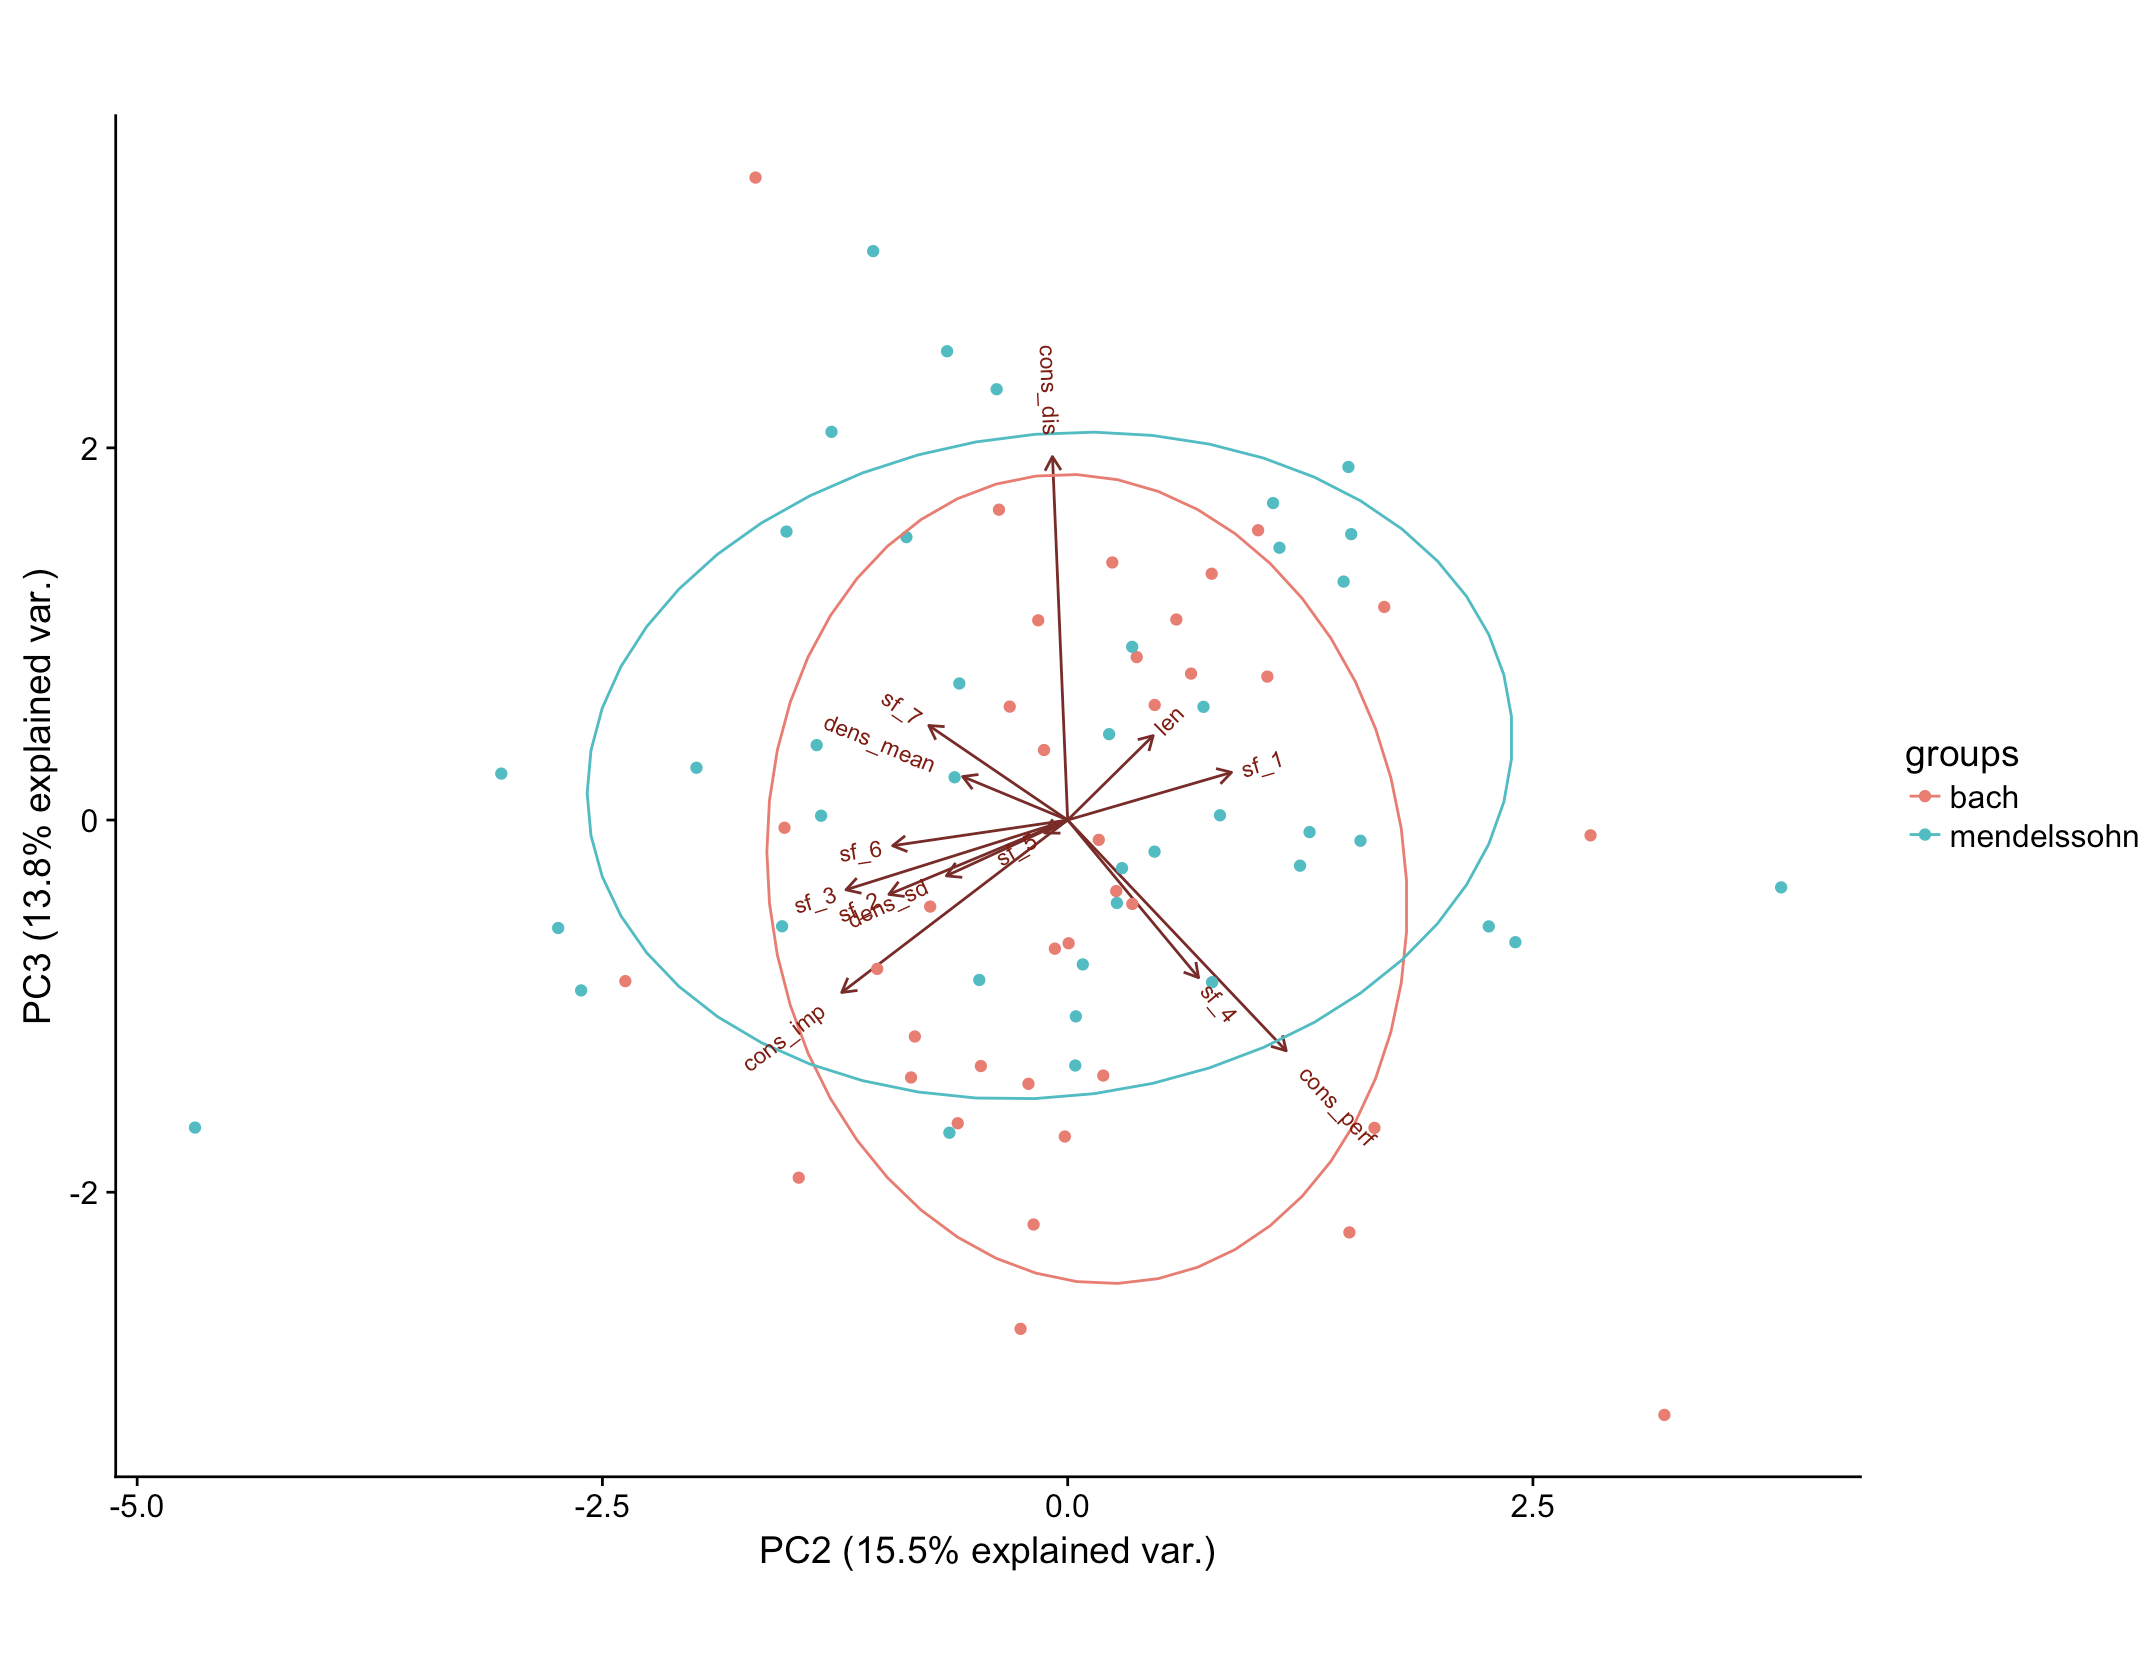
\includegraphics[scale = .3]{images/pca23bm.png}
\caption{Biplot of the second and third principal components plotted with data points colored by composer. }
\label{subd}
\end{figure}
\begin{figure}[h]
\centering
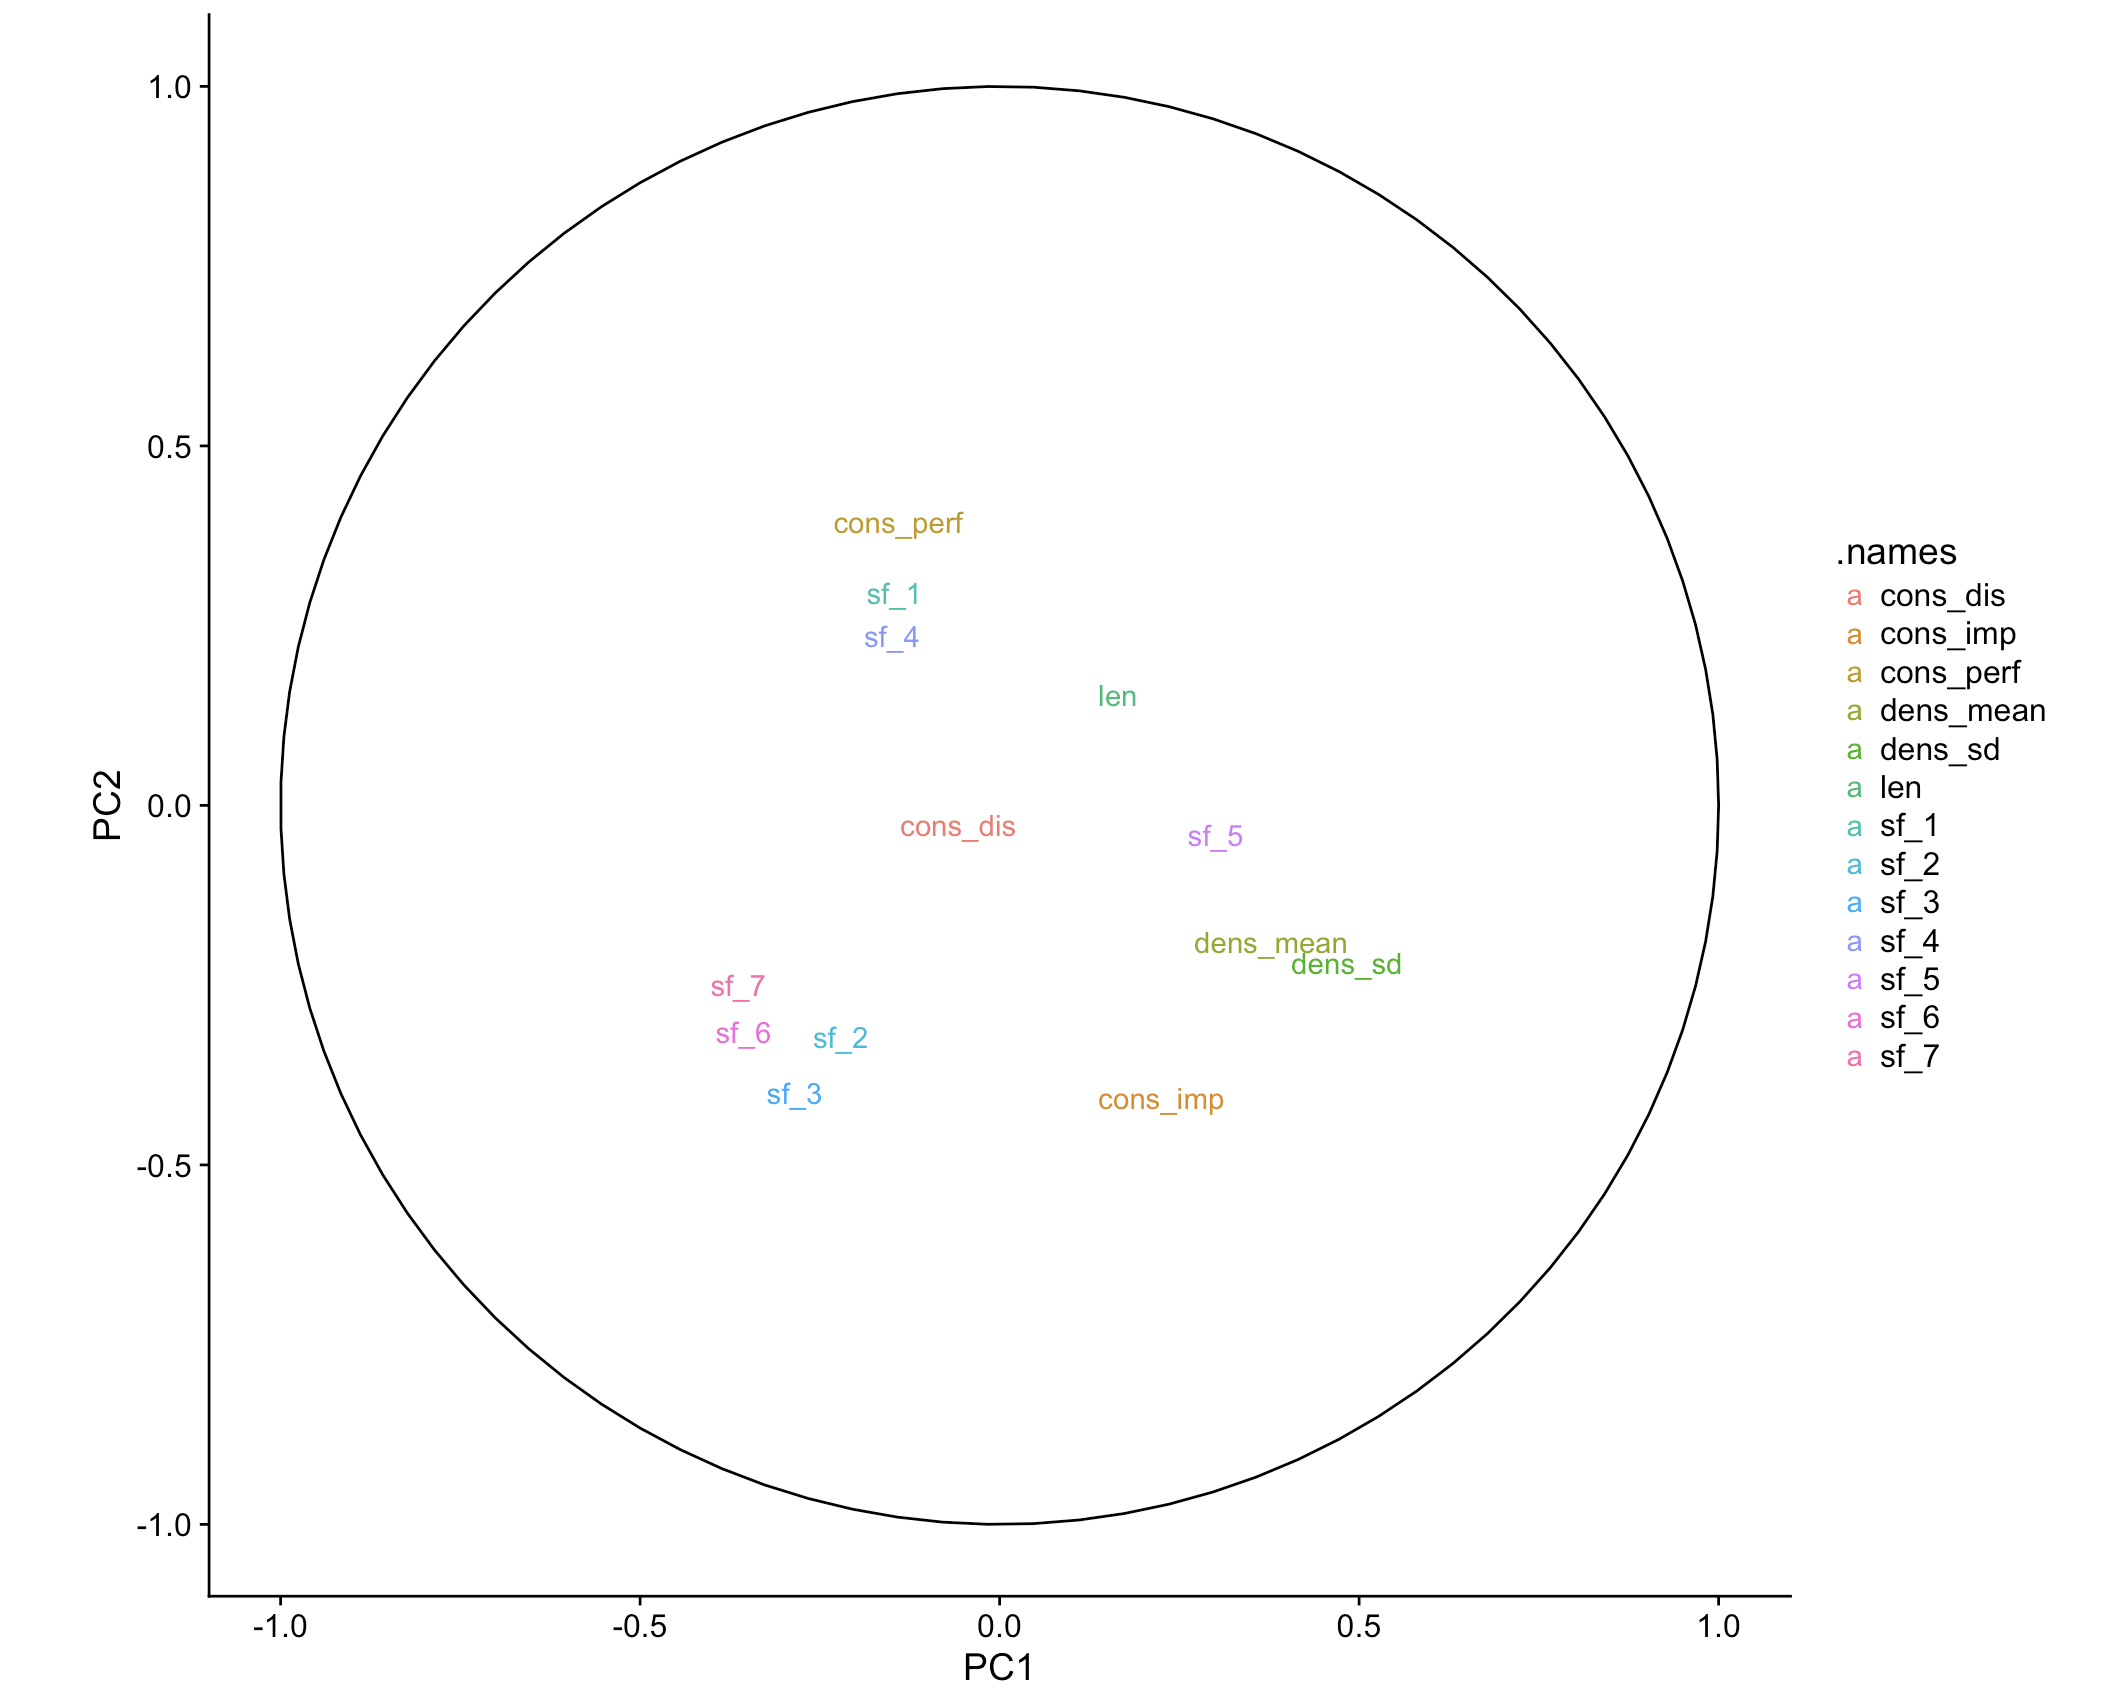
\includegraphics[scale = .3]{images/circle_bm.png}
\caption{Loadings plotted on a unit circle}
\label{subd}
\end{figure}
\begin{figure}[h]
\centering
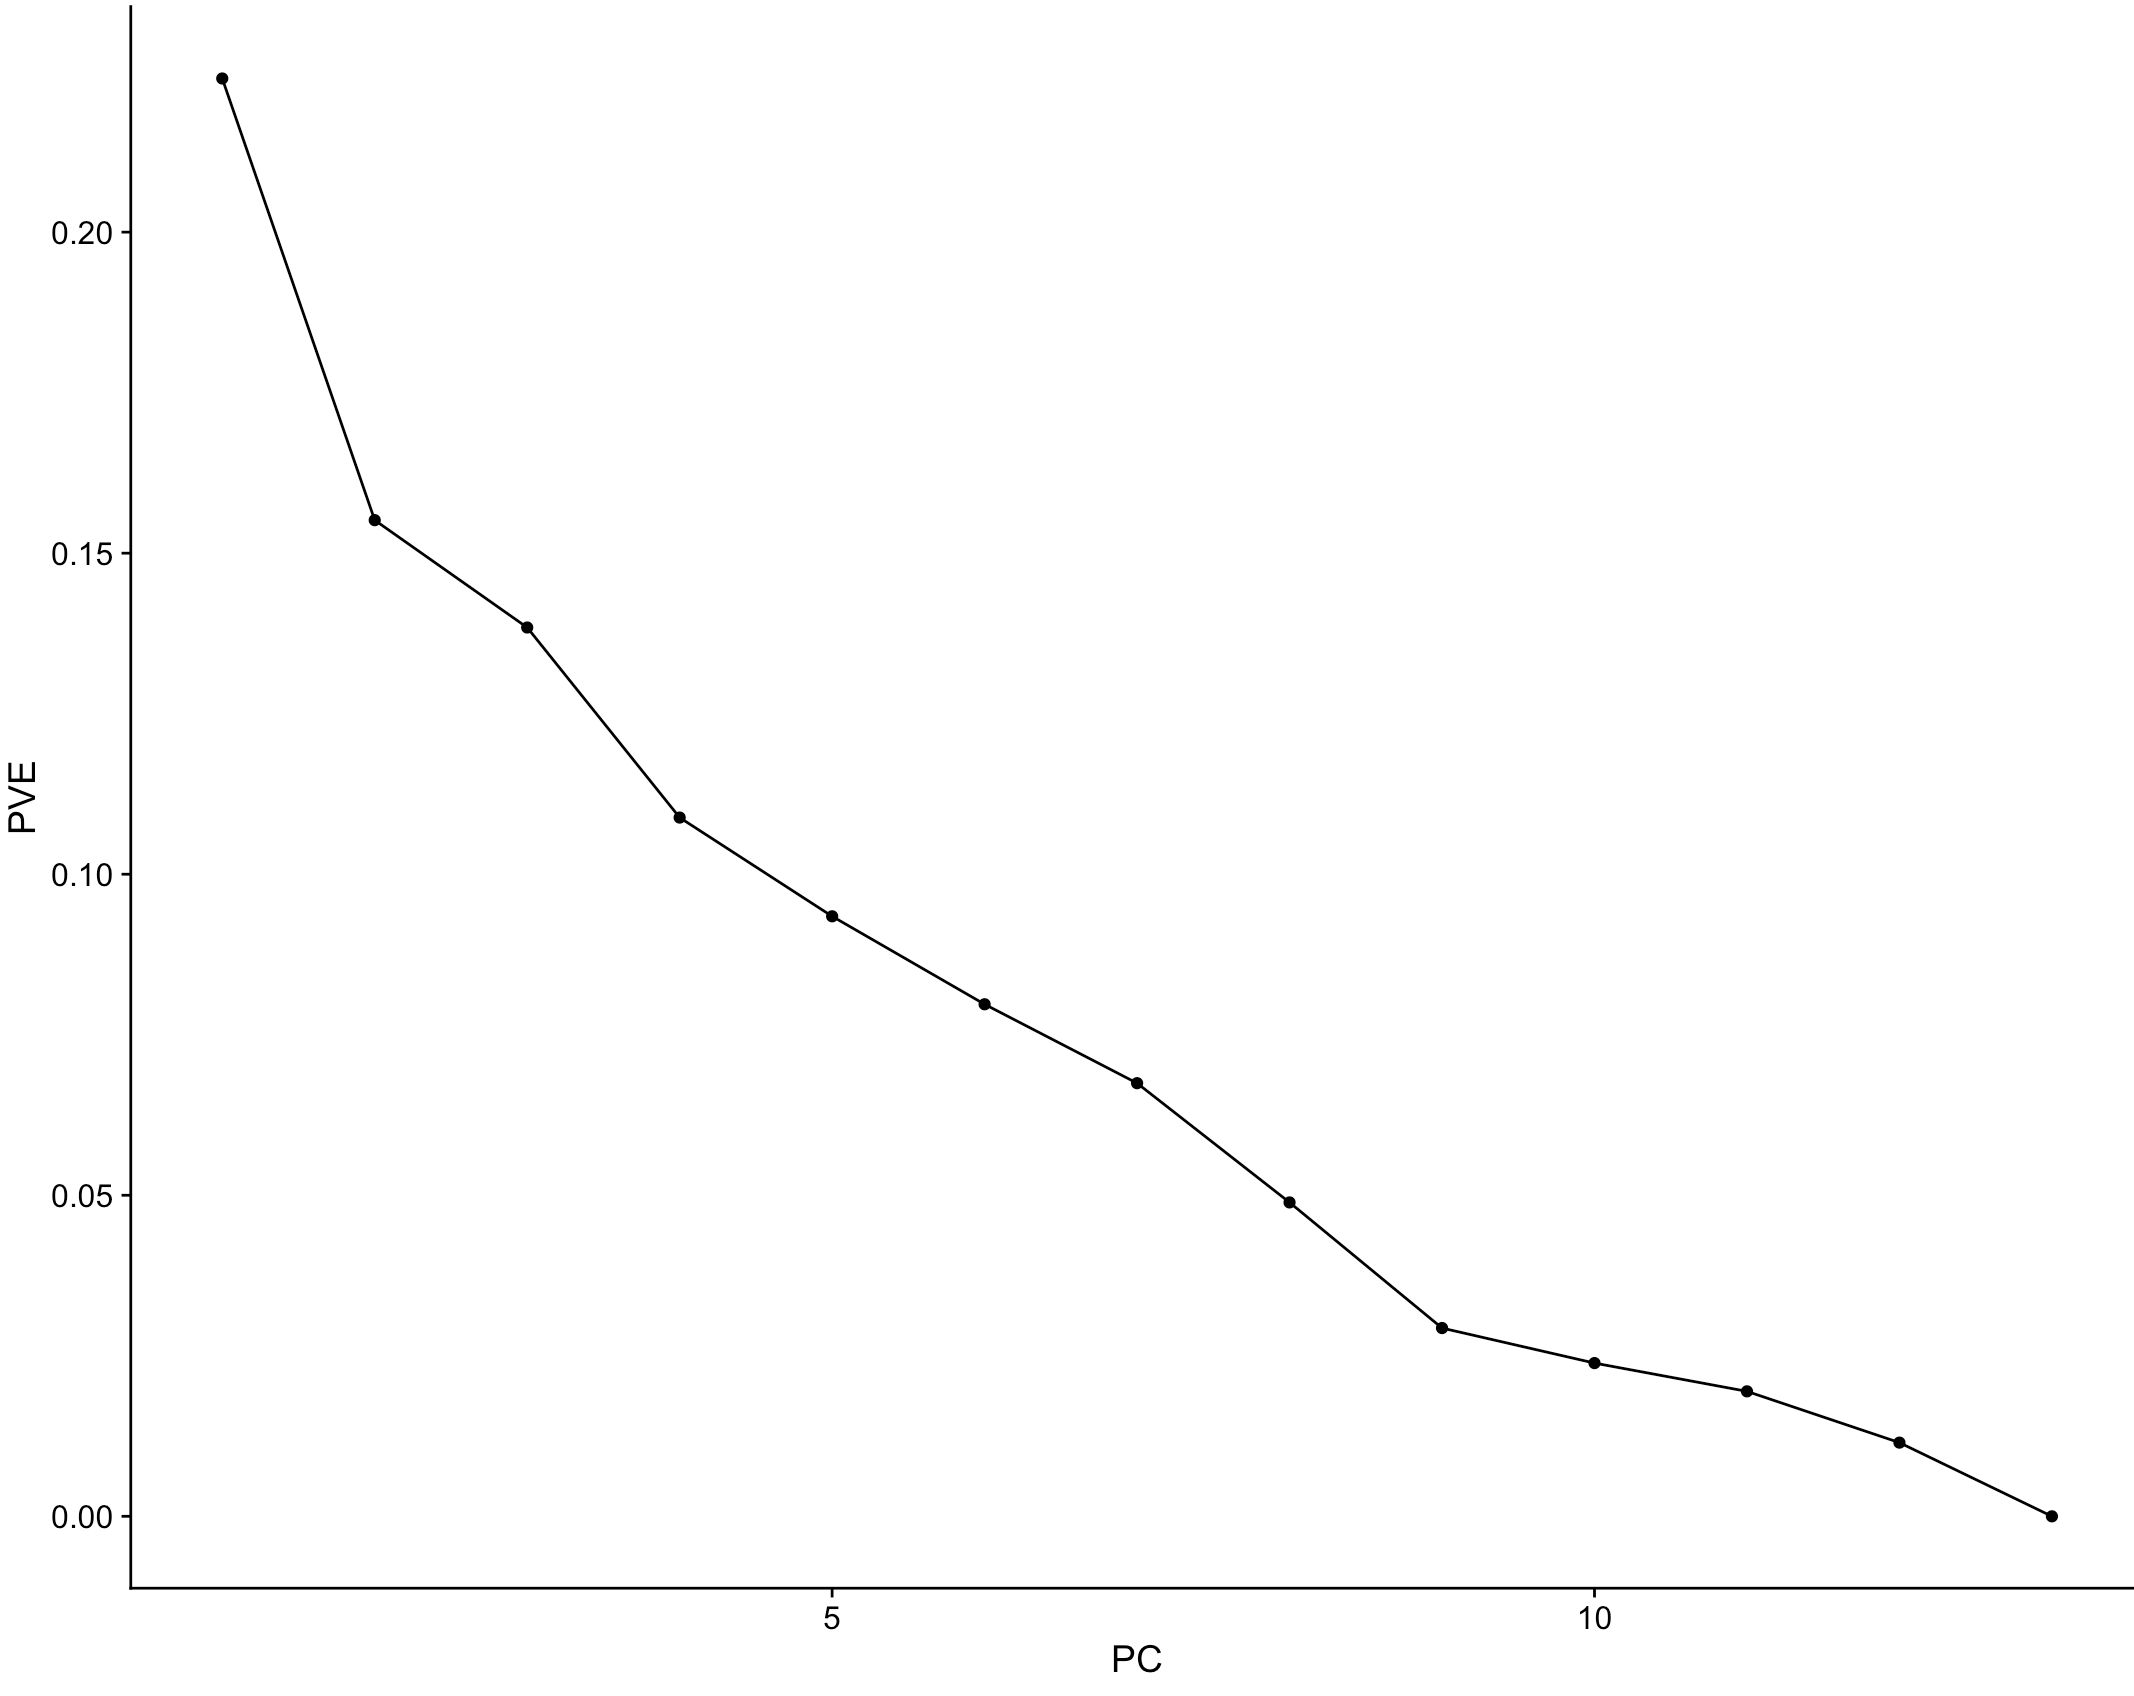
\includegraphics[scale = .3]{images/bskree.png}
\caption{Skree plot of the PCA's}
\label{subd}
\end{figure}
The skree plot shows no clear elbow. Because of this, and also because
we do not have too many predictors, we will choose to use \(p-1\)
principal components in subsequent analysis, where \(p\) is the number
of predictors in our feature space.

We can also use K-means clustering to see if there are any apparent
groups in the data. When we run K-means on the bach and mendelssohn with
K = 2 (since there are two composers)
\begin{figure}[h]
\centering
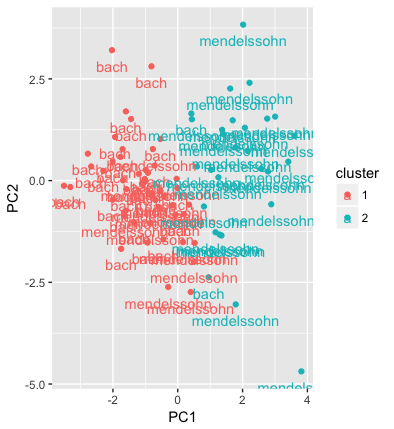
\includegraphics[scale = .3]{images/Kmeanspca.png}
\caption{KNN when k = 2}
\label{subd}
\end{figure}
We can also examine when \(K=3\), as the Mendelssohn set is made up of
fanny and felix, so there are actually three composers. (fix labeling)
\begin{figure}[h]
\centering
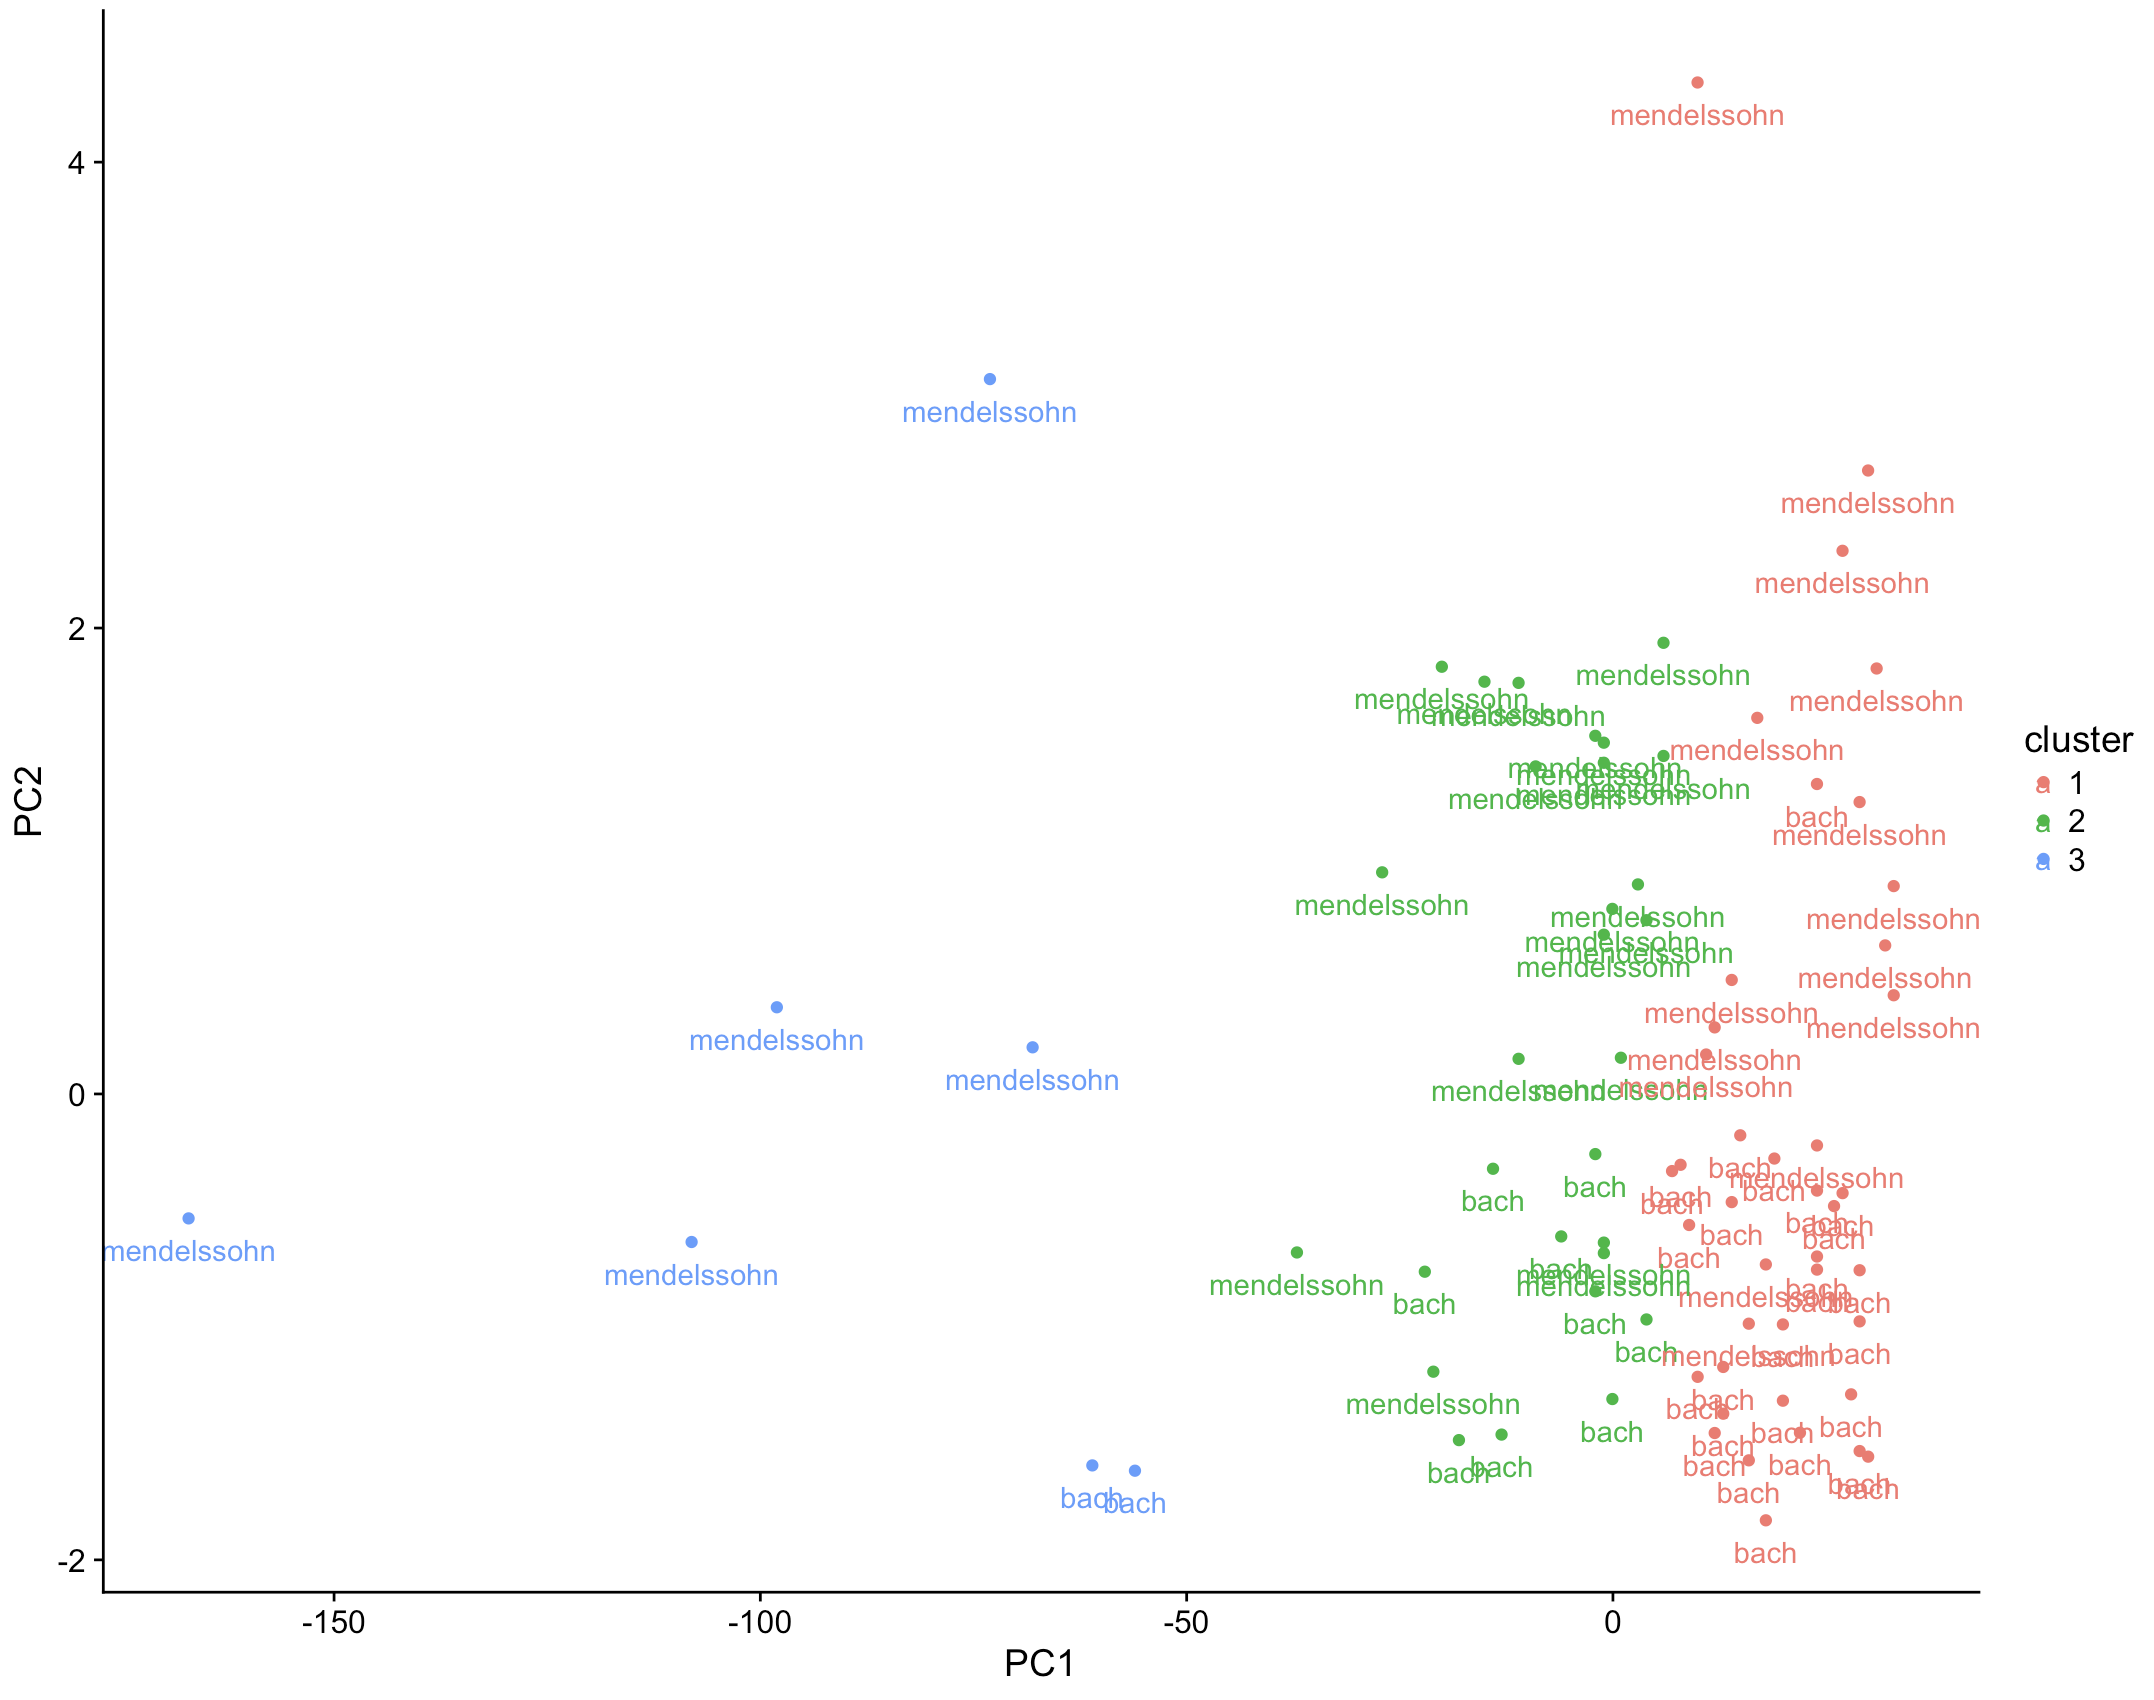
\includegraphics[scale = .3]{images/k3.png}
\caption{KNN when k = 3}
\label{subd}
\end{figure}
\section{Felix and Fanny}\label{felix-and-fanny}

There will be pairwise scatterplots of features? Which ones? Also
distributions of composer for certain features? Which ones? Who knows.

We can see from the above pairwise distribution plot that we still have
a high correlation between scale degrees 3 and 6. However we do not see
the difference in beat density. This is likely due to the fact that
fanny and Felix data set is composed of the same type of song, whereas
the Bach data set is only solo piano music.
\begin{figure}[h]
\centering
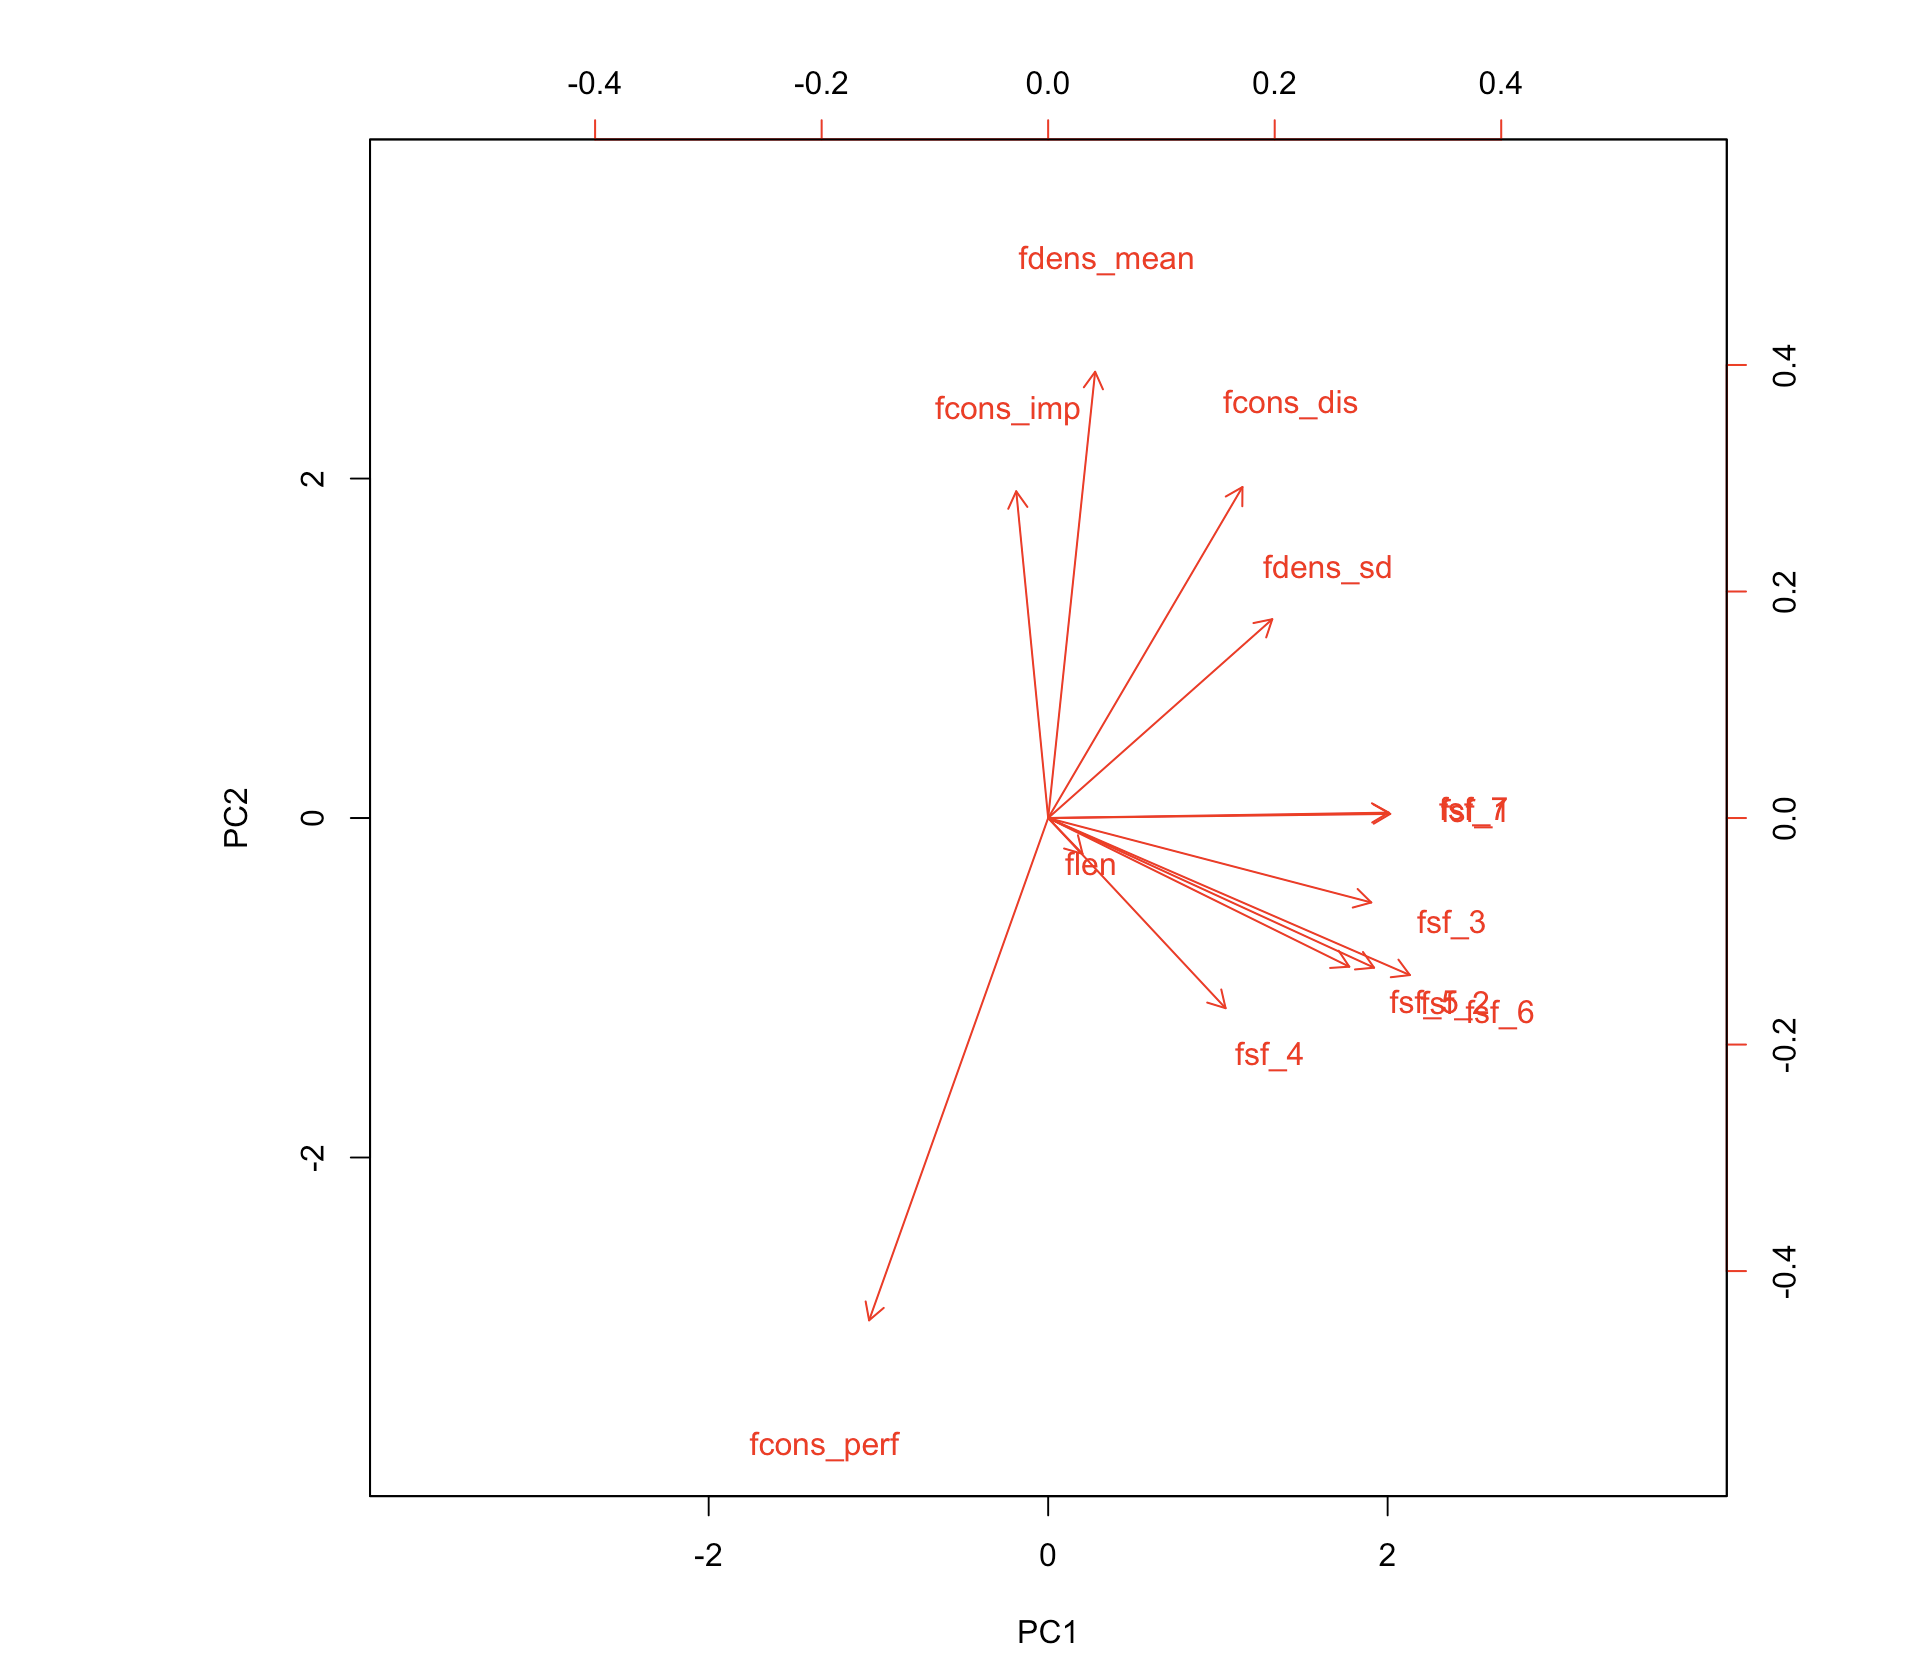
\includegraphics[scale = .3]{images/ploadff.png}
\caption{PCA Loadings of the features for Felix and Fanny}
\label{subd}
\end{figure}
There doesn't seem to be as much of a musical interpretation of the
loadings of the principal components. We do notice that the frequency of
perfect consonant melodic intervals in the voice (fcons\_perf) has an
almost opposite signs of the second principal component to the frequency
of imperfect and dissonant melodic intervals. The skree plot also doesnt
seem to show a clear elbow as indication of how many PCs to choose in
subsequent analysis.
\begin{figure}[h]
\centering
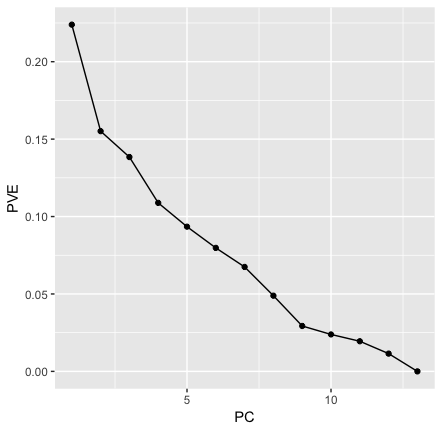
\includegraphics[scale = .5]{images/fpca_skree.png}
\caption{PCA felix/fanny skree plot}
\label{subd}
\end{figure}
\begin{figure}[h]
\centering
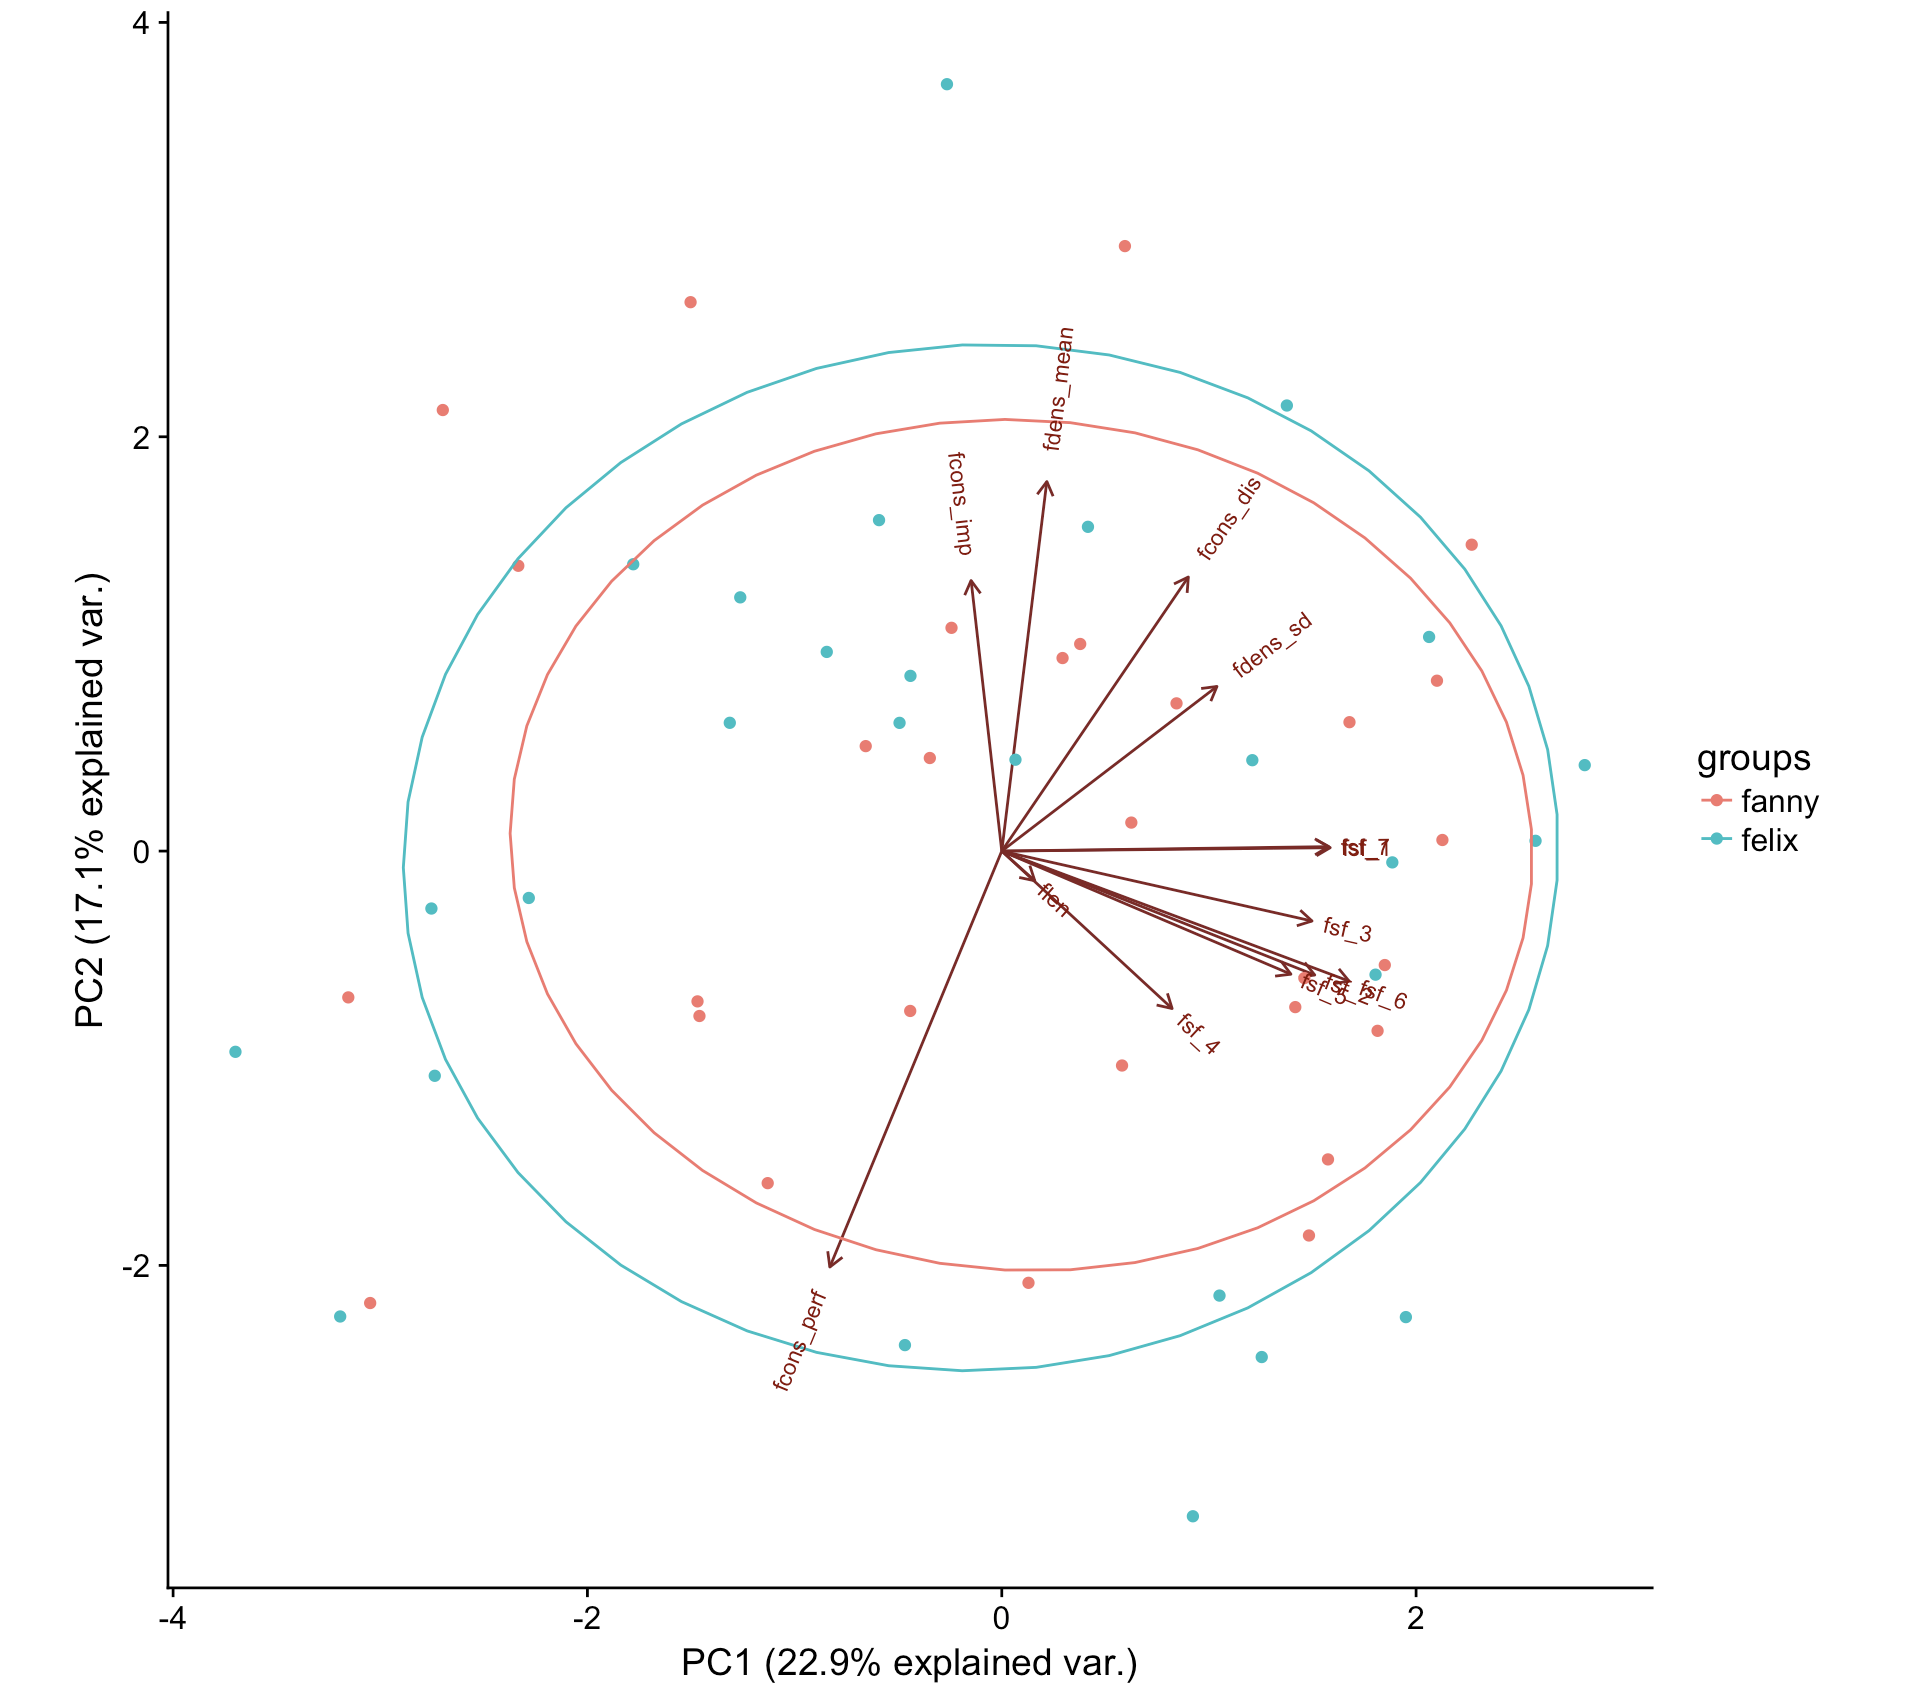
\includegraphics[scale = .3]{images/ff_elipse12.png}
\caption{Loadings and pieces plotted on the first principal components. }
\label{subd}
\end{figure}
Unfortunately, as we see in the above picutre, there is absolutely no
seperation in the groups. This might lead to issues in creating a model
to classify.
\begin{figure}[h]
\centering
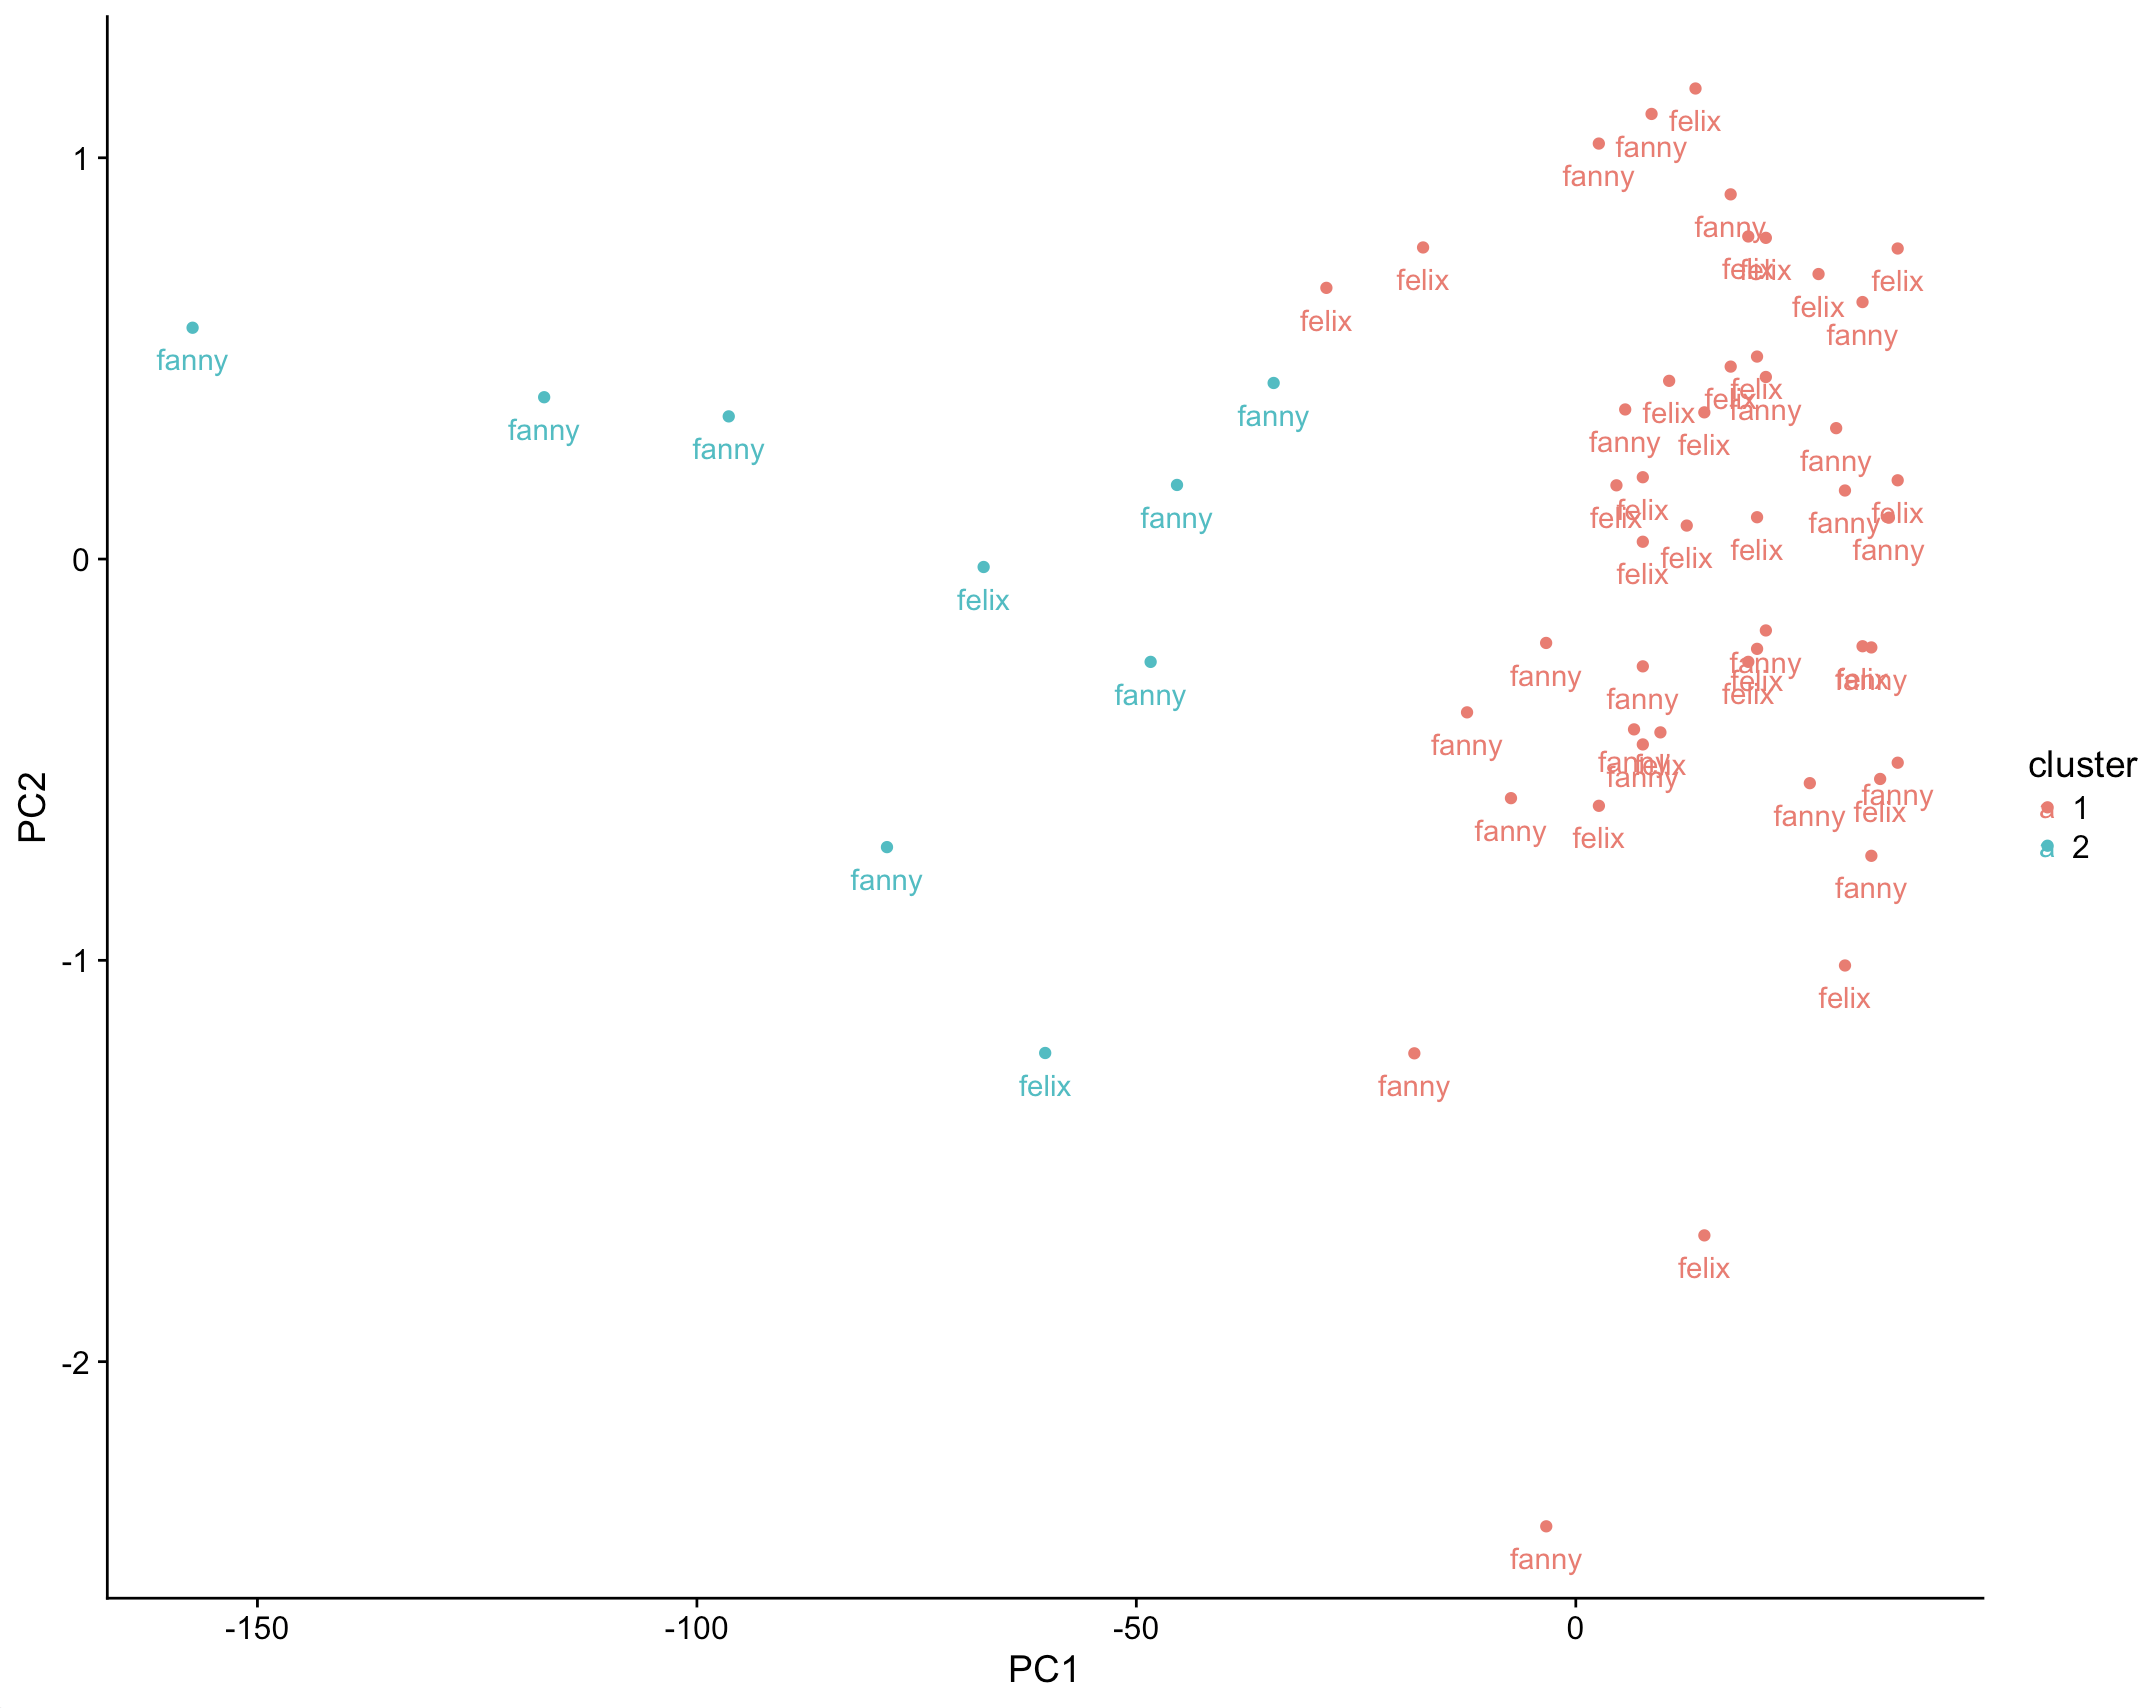
\includegraphics[scale = .3]{images/kmf.png}
\caption{K-means with k = 2}
\label{subd}
\end{figure}
When we run K-means with \(K=2\) we get the following. It does not seem
choose groups by composer.

\chapter{Model Fit}\label{model-fit}

\section{Model Fit -
Bach/Mendelssohn}\label{model-fit---bachmendelssohn}

\subsubsection{Logistic Regression}\label{logistic-regression-1}

A 5-fold cross-validated lasso logistic model was fit. The below graph
shows the miss-classification rate for different values of log(lambda).
A model fit using the lambda value with the minimum missclassifcation
rate resulted in a miss-classification rate of 0.117. We see that the
density features stayed in the longest.
\begin{figure}[h]
\centering
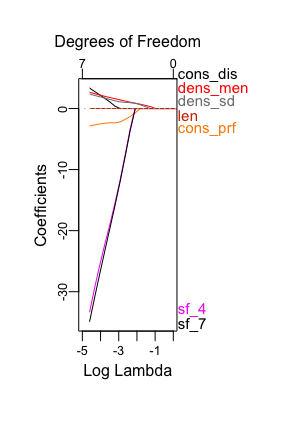
\includegraphics[scale = .5]{images/lasso_bach.png}
\caption{Lasso penalties for each feature for changing lambda penalty values}
\label{subd}
\end{figure}
\begin{figure}[h]
\centering
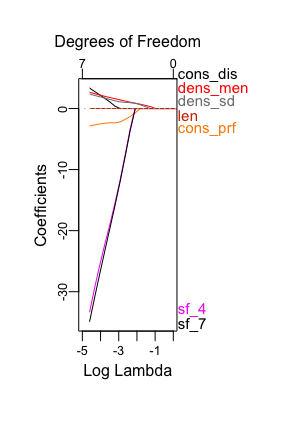
\includegraphics[scale = .5]{images/lasso_bach.png}
\caption{Cross validated misclassification rates for different lambdas. The left dotted line represents the minimum lambda, and the right line represents the lambda within one standard deviation. It is a more restricted model that can guard against over fitting, but is not used here.}
\label{subd}
\end{figure}
\subsubsection{LDA}\label{lda}

For linear discriminant analysis, we have a 5-fold cross validated MSE
of 0.13.Most commonly our models incorrectly predict Mendelssohn songs
to be composed by Bach.

\subsubsection{Naive Bayes}\label{naive-bayes-1}

A naive model was fit and resulted a miss-classification rate of 0.07

\subsubsection{KNN}\label{knn}

A K-Nearest Neighbors classifier was fit, with \(K\) chosen to be 1 from
5-fold cross validation. This resulted in a miss-classification rate of
.22

\section{Model fit Felix/Fanny}\label{model-fit-felixfanny}

It there seems like there is not enough data to have a stable
missclassification rate for different choices of fold.

\subsubsection{Logistic regression}\label{logistic-regression-2}

When a logistic classifier was fit, we got an average
miss-classification rate of 0.35. We see that the density features and
fifth scale degree stayed in the longest.

\subsubsection{Naive Bayes}\label{naive-bayes-2}

A naive Bayes model was fit and the 5-fold miss-classification rate
averaged between .4 and .5.

\subsubsection{LDA}\label{lda-1}

An LDA model was fit and predicts correctly about 50/50

\subsubsection{knn}\label{knn-1}

With K=8, the missclassification rate was about .43

\section{Predictions for Disputed
pieces:}\label{predictions-for-disputed-pieces}

Since we have such high missclassification rates, the following
predictions are likely not accurate.
\begin{itemize}
\tightlist
\item
  Logistic: Predicts Op 8 no 2 and 12 to be written by Felix.
\item
  Naive Bayes: Predicted all four as written by Fanny.
\item
  knn: Predicted Op 8 no 12 to be written by Felix.
\item
  LDA: Predicted Op9 no 12 to be written by Felix.
\end{itemize}
\chapter{Discussion}\label{discussion}

\section{Discussion}\label{discussion-1}

On very basic low-level features, consiting mostly of frequencies of
notes, intervals and chords, most models comparing Bach to the
Mendelssohns do relatively well. This is likely due to the decent
seperation of the feature encoding density as shown below. This is
likely because the Bach data is for solo piano and the Mendelssohn data
has an additional instrument, thus makeing the piece automatically more
dense.
\begin{figure}[h]
\centering
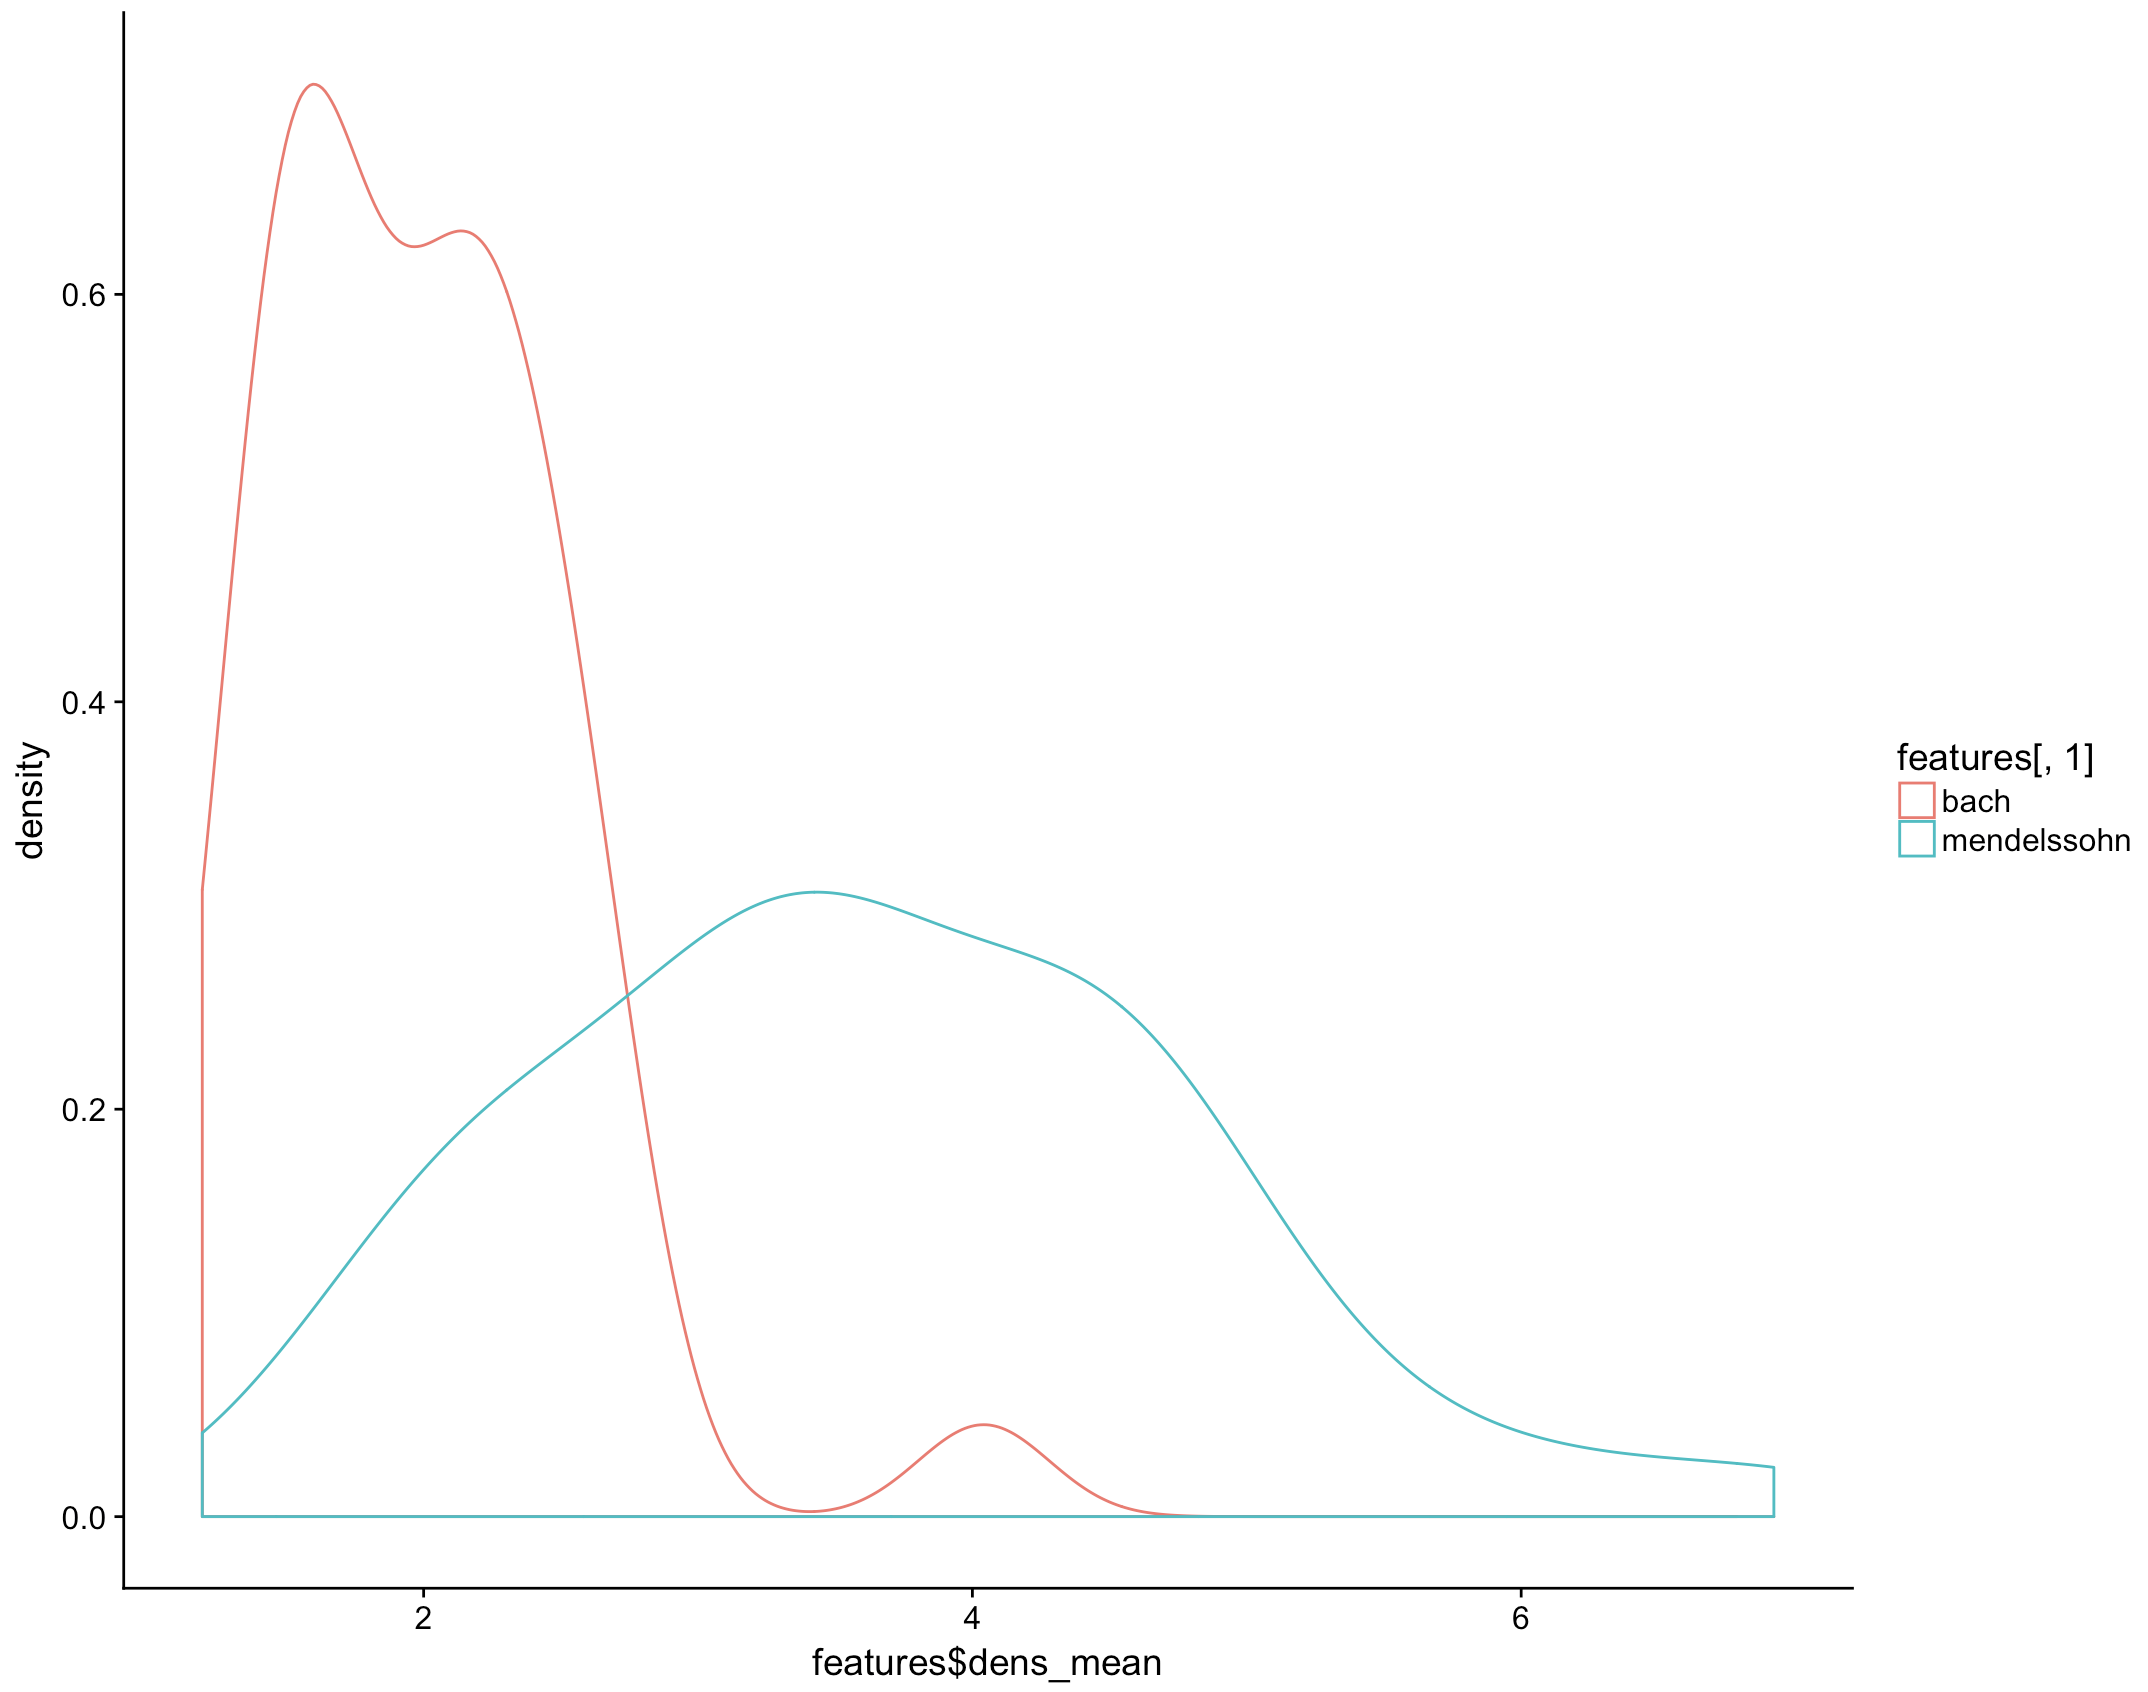
\includegraphics[scale = .5]{images/dens.png}
\caption{Distribution of feature of the mean beat density for Bach and Mendelssohn}
\label{subd}
\end{figure}
\begin{longtable}[]{@{}ll@{}}
\caption{Miss-classification Rates for differnt models comparing Bach
and Mendelssohns}\tabularnewline
\toprule
Model & Miss-classification Rate\tabularnewline
\midrule
\endfirsthead
\toprule
Model & Miss-classification Rate\tabularnewline
\midrule
\endhead
Naive Bayes & 0\tabularnewline
KNN & 0\tabularnewline
LDA & 0\tabularnewline
Logistic & 0\tabularnewline
\bottomrule
\end{longtable}
On the other hand, models fit to compare Felix and Fanny did not do as
well. They are only very slightly better than random guessing.
\begin{longtable}[]{@{}ll@{}}
\caption{Miss-classification Rates for differnt models comparing Felix
and Fanny}\tabularnewline
\toprule
Model & Miss-classification Rate\tabularnewline
\midrule
\endfirsthead
\toprule
Model & Miss-classification Rate\tabularnewline
\midrule
\endhead
Naive Bayes & 0\tabularnewline
KNN & 0\tabularnewline
LDA & 0\tabularnewline
Logistic & 0\tabularnewline
\bottomrule
\end{longtable}
\section{Future suggestions for
museR}\label{future-suggestions-for-muser}

Future suggestions to improve functionality of the R package museR
include equipping it to deal with higher level features\ldots{}

\chapter*{Conclusion}\label{conclusion}
\addcontentsline{toc}{chapter}{Conclusion}

\appendix

\chapter{The First Appendix}\label{the-first-appendix}

This first appendix includes all of the R chunks of code that were
hidden throughout the document (using the \texttt{include\ =\ FALSE}
chunk tag) to help with readibility and/or setup.

\textbf{In the main Rmd file}
\begin{Shaded}
\begin{Highlighting}[]
\CommentTok{# This chunk ensures that the thesisdown package is}
\CommentTok{# installed and loaded. This thesisdown package includes}
\CommentTok{# the template files for the thesis.}
\ControlFlowTok{if}\NormalTok{(}\OperatorTok{!}\KeywordTok{require}\NormalTok{(devtools))}
  \KeywordTok{install.packages}\NormalTok{(}\StringTok{"devtools"}\NormalTok{, }\DataTypeTok{repos =} \StringTok{"http://cran.rstudio.com"}\NormalTok{)}
\ControlFlowTok{if}\NormalTok{(}\OperatorTok{!}\KeywordTok{require}\NormalTok{(thesisdown))}
\NormalTok{  devtools}\OperatorTok{::}\KeywordTok{install_github}\NormalTok{(}\StringTok{"ismayc/thesisdown"}\NormalTok{)}
\KeywordTok{library}\NormalTok{(thesisdown)}
\KeywordTok{library}\NormalTok{(MASS)}
\KeywordTok{library}\NormalTok{(class)}
\KeywordTok{library}\NormalTok{(tidyverse)}
\KeywordTok{library}\NormalTok{(tree)}
\KeywordTok{library}\NormalTok{(randomForest)}
\KeywordTok{library}\NormalTok{(e1071)}
\KeywordTok{library}\NormalTok{(ggplot2)}
\KeywordTok{library}\NormalTok{(GGally)}
\KeywordTok{library}\NormalTok{(ISLR)}
\KeywordTok{library}\NormalTok{(boot)}
\KeywordTok{library}\NormalTok{(glmnet)}
\KeywordTok{library}\NormalTok{(caret)}
\KeywordTok{library}\NormalTok{(plotmo)}
\KeywordTok{library}\NormalTok{(museR)}
\end{Highlighting}
\end{Shaded}
\textbf{In Chapter \ref{ref-labels}:}

\backmatter

\chapter*{References}\label{references}
\addcontentsline{toc}{chapter}{References}

\markboth{References}{References}

\noindent

\setlength{\parindent}{-0.20in} \setlength{\leftskip}{0.20in}
\setlength{\parskip}{8pt}

\hypertarget{refs}{}
\hypertarget{ref-adair1944}{}
Adair, D. (1944). The authorship of the disputed federalist papers.
\emph{The William and Mary Quarterly: A Magazine of Early American
History,} 98--122.

\hypertarget{ref-harmonicon}{}
Ayrton, W. (1830). \emph{The harmonicon} (Vol. 8). W. Pinnock.

\hypertarget{ref-backer2005}{}
Backer, E., \& Kranenburg, P. van. (2005). On musical stylometry---a
pattern recognition approach. \emph{Pattern Recognition Letters},
\emph{26}(3), 299--309.

\hypertarget{ref-brinkman2016}{}
Brinkman, A., Shanahan, D., \& Sapp, C. (n.d.). Musical stylometry,
machine learning, and attribution studies: A semi-supervised approach to
the works of josquin.

\hypertarget{ref-OMR}{}
Doermann, D., Tombre, K., \& others. (2014). \emph{Handbook of document
image processing and recognition}. Springer.

\hypertarget{ref-authorshipfed}{}
Ford, P. L., \& Bourne, E. G. (1897). The authorship of the federalist.
\emph{The American Historical Review}, \emph{2}(4), 675--687. Retrieved
from \url{http://www.jstor.org/stable/1833983}

\hypertarget{ref-esl}{}
Friedman, J., Hastie, T., \& Tibshirani, R. (2001). \emph{The elements
of statistical learning} (Vol. 1). Springer series in statistics New
York.

\hypertarget{ref-guyon2003}{}
Guyon, I., \& Elisseeff, A. (2003). An introduction to variable and
feature selection. \emph{Journal of Machine Learning Research},
\emph{3}(Mar), 1157--1182.

\hypertarget{ref-isl}{}
James, G., Witten, D., Hastie, T., \& Tibshirani, R. (2013). \emph{An
introduction to statistical learning} (Vol. 112). Springer.

\hypertarget{ref-mace2013}{}
Mace, A. R. (2013). \emph{Fanny hensel, felix mendelssohn bartholdy, and
the formation of the`` mendelssohnian'' style} (PhD thesis).

\hypertarget{ref-mearns2010}{}
Mearns, L., Tidhar, D., \& Dixon, S. (2010). Characterisation of
composer style using high-level musical features. In \emph{Proceedings
of 3rd international workshop on machine learning and music} (pp.
37--40). ACM.

\hypertarget{ref-mosteller1964inference}{}
Mosteller, F., \& Wallace, D. (1964). \emph{Inference and disputed
authorship: The federalist}. Addison-Wesley.

\hypertarget{ref-papadopoulosai}{}
Papadopoulos, G., \& Wiggins, G. (n.d.). AI methods for algorithmic
composition: A survey, a critical view and future prospects.

\hypertarget{ref-pudil1994floating}{}
Pudil, P., Novovičová, J., \& Kittler, J. (1994). Floating search
methods in feature selection. \emph{Pattern Recognition Letters},
\emph{15}(11), 1119--1125.

\hypertarget{ref-reich1991}{}
Reich, N. B. (1991). The power of class: Fanny hensel. \emph{Mendelssohn
and His World}, 86--99.

\hypertarget{ref-CompStyleAttri}{}
Speiser, J., \& Gupta, V. (n.d.). Composer style attribution.
\emph{Project Report for CS}, \emph{229}.

\hypertarget{ref-jrp}{}
The josquin research project. (n.d.). \emph{The Josquin Research
Project}. Retrieved from \url{http://josquin.stanford.edu/}

\hypertarget{ref-lasso}{}
Tibshirani, R. (1996). Regression shrinkage and selection via the lasso.
\emph{Journal of the Royal Statistical Society. Series B
(Methodological)}, 267--288.

\hypertarget{ref-tillard1996}{}
Tillard, F. (1996). \emph{Fanny mendelssohn}. Hal Leonard Corporation.

\hypertarget{ref-todd2003}{}
Todd, R. L. (2003). \emph{Mendelssohn: A life in music}. Oxford
University Press.


% Index?

\end{document}
